\phantomsection
\definecolor{dkgreen}{rgb}{0,0.6,0}
\definecolor{gray}{rgb}{0.5,0.5,0.5}
\definecolor{mauve}{rgb}{0.58,0,0.82}


\lstset{frame=tb,
language=R,
aboveskip=3mm,
belowskip=3mm,
showstringspaces=false,
columns=flexible,
numbers=none,
inputencoding=utf8/latin1,
keywordstyle=\color{blue},
numberstyle=\tiny\color{gray},
commentstyle=\color{dkgreen},
stringstyle=\color{mauve},
breaklines=true,
breakatwhitespace=true,
tabsize=3
}

\chapter{Grafici}\label{cap2} %\label{1cap:spinta_laterale}

In questo capitolo verranno mostrati \textbf{grafici a barre} e \textbf{grafici a torta} per rappresentare i dati del dataset, evidenziandone le principali caratteristiche.

Il dataset sarà analizzato con grafici sia in base alle singole regioni, sia in base alle singole caratteristiche.

\section{Grafici a barre: Caratteristiche}\label{cap2.1}

In questa sezione verrà mostrato un grafico a barre per ogni caratteristica del dataset, al fine di poter confrontare tra le varie regioni le abitudini principali delle persone; inoltre, ogni grafico sarà correlato con la propria media campionaria.

\vspace{5mm}
\noindent \textbf{Costruzione del grafico a barre}

Per la costruzione di un grafico a barre si utilizzano le seguenti linee di codice:

\vspace{5mm}
\begin{lstlisting}
  bp1 <- barplot(df$Modo.Cont., main = "Persone che praticano sport in modo continuativo nelle regioni", col = rainbow(20))
  abline(h = mean(df$Modo.Cont.), lty = 2, col = "red")
  text(bp1, par("usr")[3], labels = row.names(df), srt = 45, adj = c(1, 1), xpd = TRUE, cex = 0.8)

  bp1 <- barplot(df$Modo.Salt., main = "Persone che praticano sport in modo saltuario nelle regioni", col = rainbow(20))
  abline(h = mean(df$Modo.Salt.), lty = 2, col = "red")
  text(bp1, par("usr")[3], labels = row.names(df), srt = 45, adj = c(1, 1), xpd = TRUE, cex = 0.8)

  bp1 <- barplot(df$Qualche.Att., main = "Persone che praticano solo qualche attività fisica nelle regioni", col = rainbow(20))
  abline(h = mean(df$Qualche.Att.), lty = 2, col = "red")
  text(bp1, par("usr")[3], labels = row.names(df), srt = 45, adj = c(1, 1), xpd = TRUE, cex = 0.8)

  bp1 <- barplot(df$Non.Prat.Sport., main = "Persone che non praticano sport nelle regioni", col = rainbow(20))
  abline(h = mean(df$Non.Prat.Sport.), lty = 2, col = "red")
  text(bp1, par("usr")[3], labels = row.names(df), srt = 45, adj = c(1, 1), xpd = TRUE, cex = 0.8)

\end{lstlisting}
\vspace{5mm}

Dove la variabile \textit{bp1} memorizza un barplot relativo alla frequenza delle attività sportive nelle varie regioni. I dati del dataset sono recuperati attraverso \textit{df\$Modo.Cont.}, mentre ulteriori caratteristiche associate al grafico, come il titolo e i colori da utilizzare per le barre sono gestite rispettivamente dai parametri \textit{main} e \textit{col}. Per evidenziare, invece, la media di tale caratteristica sul grafico è stata aggiunta una retta attraverso la funzione \textit{abline()}. Infine, tramite la funzione \textit{text()}, sono stati aggiunti i nomi delle regioni italiane sull’asse x, ponendoli in modo tale da essere visualizzati per intero.

Di seguito per ciascuna caratteristica il grafico a barre viene costruito con il medesimo codice sopra descritto, sostituendo soltanto il parametro \textit{df\$Modo.Cont.}. con quello della caratteristica presa in osservazione.

\begin{figure}[!htbp]
    \centering
    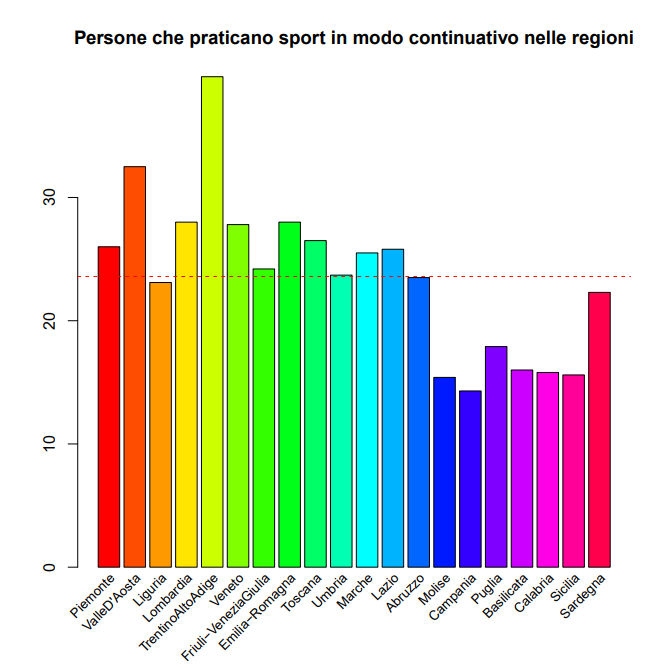
\includegraphics[height=15cm]{ProgettoSAD/capitoli/images/barre_modocont.png}
    \captionsetup{font={footnotesize,bf,it}}
    \label{fig:barre_modocont}
\end{figure}

Si può notare dal grafico che, per quanto riguarda le persone che svolgono attività fisica in modo continuativo, più della metà delle regioni superano la media campionaria, principalmente nel Nord e nel Centro dell'Italia. Il picco più alto è presente nel Trentino Alto Adige, mentre il più basso in Campania.

\begin{figure}[!htbp]
    \centering
    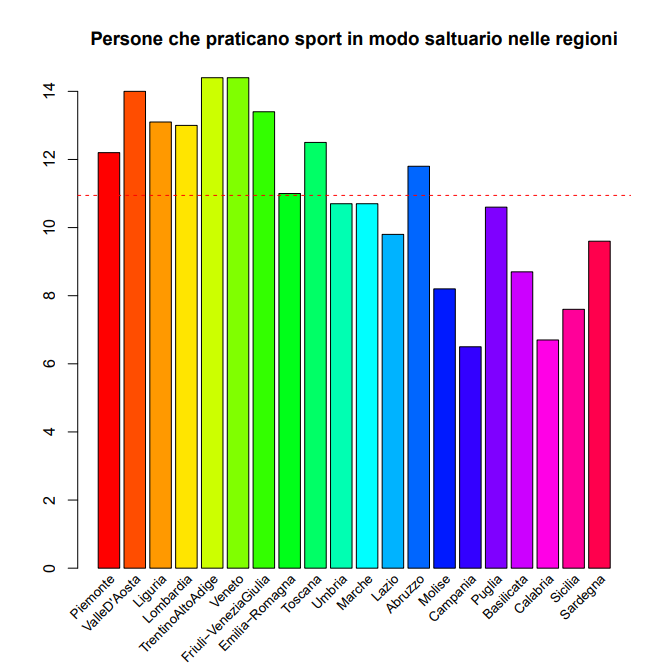
\includegraphics[height=15cm]{ProgettoSAD/capitoli/images/barre_modosalt.png}
    \captionsetup{font={footnotesize,bf,it}}
    \label{fig:barre_modosalt}
\end{figure}

Si può notare dal grafico che, per quanto riguarda le persone che svolgono attività fisica in modo saltuario, meno della metà delle regioni superano la media campionaria, principalmente nel Nord e nel Centro dell'Italia. Si evidenzia che il picco più alto è presente nel Trentino Alto Adige e nel Veneto a parità di persone, mentre il più basso in Campania.

\begin{figure}[!htbp]
    \centering
    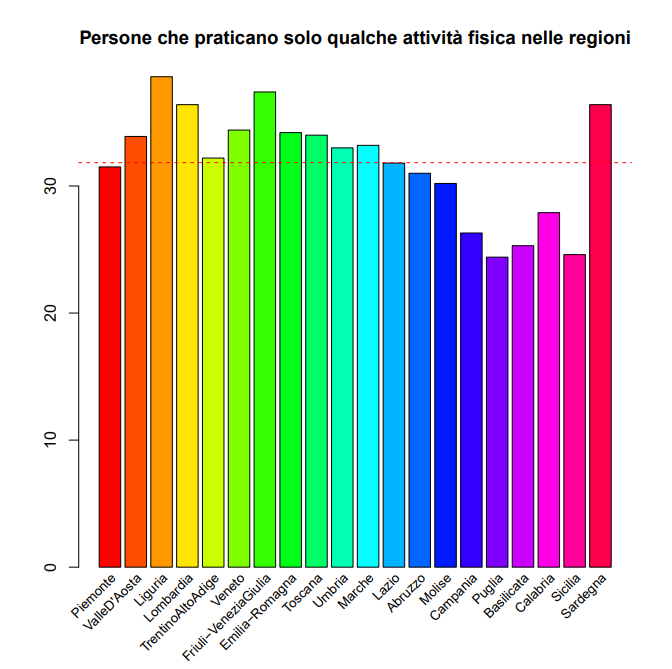
\includegraphics[height=15cm]{ProgettoSAD/capitoli/images/barre_qualcheatt.png}
    \captionsetup{font={footnotesize,bf,it}}
    \label{fig:barre_qualcheatt}
\end{figure}

Si può notare dal grafico che, per quanto riguarda le persone che svolgono qualche attività fisica, meno della metà delle regioni superano la media campionaria, principalmente nel Nord e Centro Italia e la Sardegna. Si evidenzia che il picco più alto è presente in Liguria, mentre il più basso in Puglia.

\begin{figure}[!htbp]
    \centering
    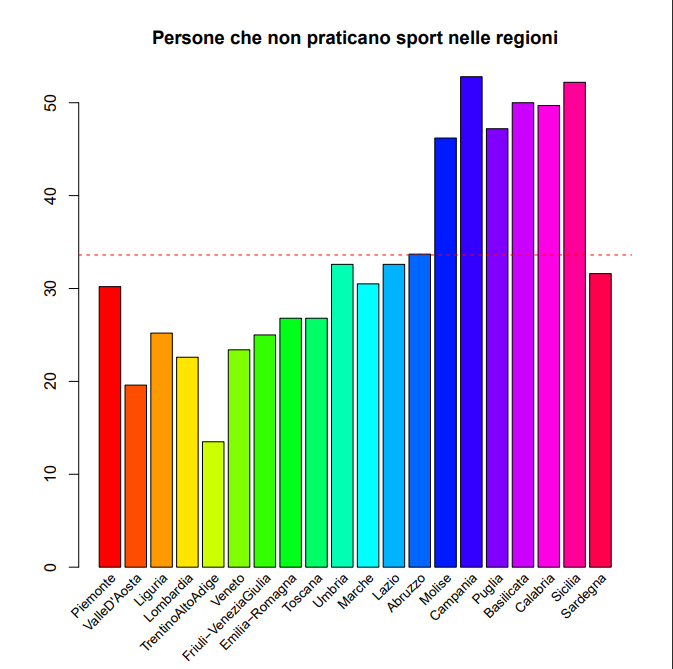
\includegraphics[height=15cm]{ProgettoSAD/capitoli/images/barre_nonpratsport.png}
    \captionsetup{font={footnotesize,bf,it}}
    \label{fig:barre_nonpratsport}
\end{figure}

Si può notare dal grafico che, per quanto riguarda le persone che non svolgono attività sportiva nelle regioni, la media campionaria viene superata da sei regioni, tutte del Sud Italia con la Sicilia. Il picco più alto è registrato in Campania, mentre il più basso in Trentino.

\section{Grafici a barre: Regioni}\label{cap2.2}

In questa sezione verrà mostrato un grafico a barre per ogni regione del dataset al fine di poter confrontare in ognuna di esse la frequenza di attività fisica tra le persone.

Per recuperare le informazioni di ogni singola regione si devono individuare le righe del dataset. Viene creata dunque una funzione per estrarre delle righe in maniera diretta.

Passando in input alla funzione \textit{estraiRiga()} l'indice di riga i e il dataframe, la funzione ritornerà i dati relativi alla i-esima riga del dataset memorizzati in un vettore.

\vspace{5mm}
\begin{lstlisting}
estraiRiga <- function(df, index) {
  vect <- c()
  for (i in df[index,]) {
    vect <- c(vect, i)
  }
  vect
}
\end{lstlisting}
\vspace{5mm}

\noindent \textbf{Costruzione Grafico a barre}

Utilizzando la funzione appena mostrata si è in grado di creare i grafici a barre per le caratteristiche.

\vspace{5mm}
\begin{lstlisting}
  index <- 1
  for (element in regioni) {
    bp1 <- barplot(estraiRiga(df, index),
                   main = element,
                   col = rainbow(4))
    abline(h = mean(estraiRiga(df, index)),
           lty = 2, col = "red")
    text(bp1, par("usr")[3],
         labels = names(df),
         srt = 45,
         adj = c(1.1, 1.1),
         xpd = TRUE, cex = 0.7)
    index <- index + 1
\end{lstlisting}
\vspace{5mm}

\begin{figure}[!htbp]
    \centering
        \subfloat{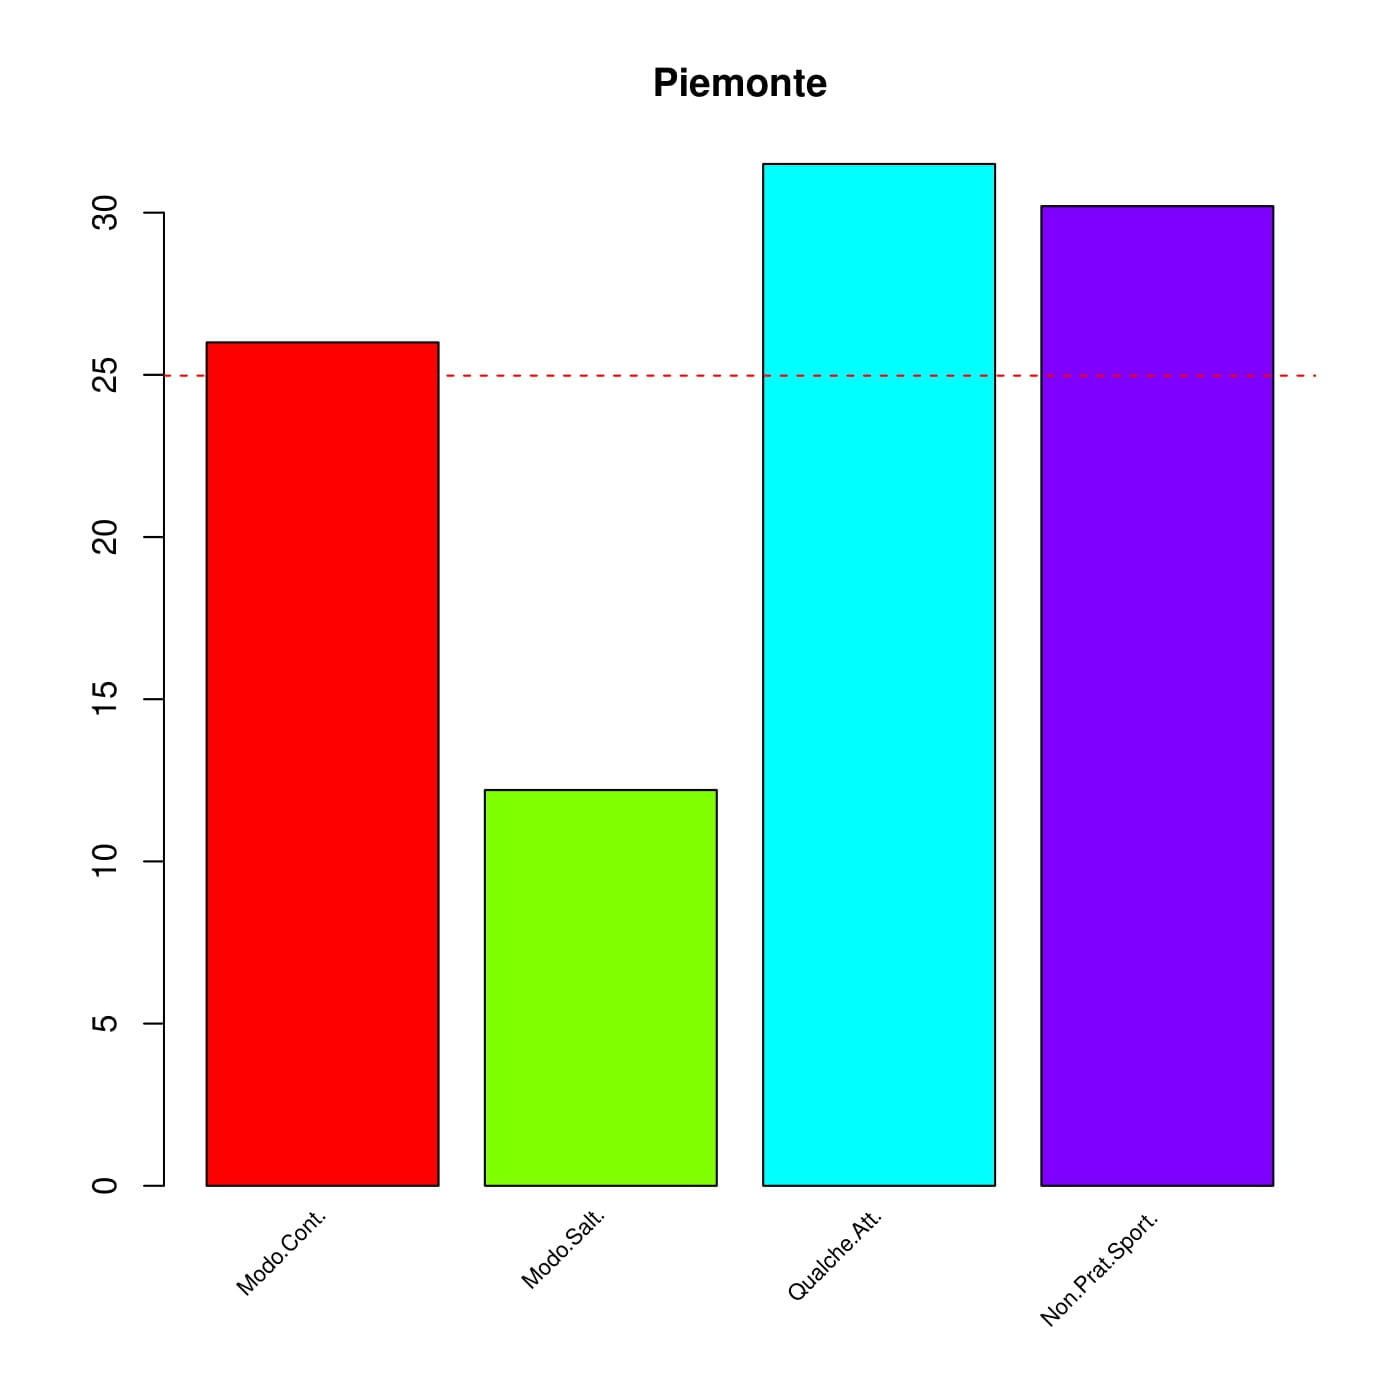
\includegraphics[height=8cm]{ProgettoSAD/capitoli/images/barre_regioni/barre_piemonte.jpg}}
        \qquad
        \subfloat{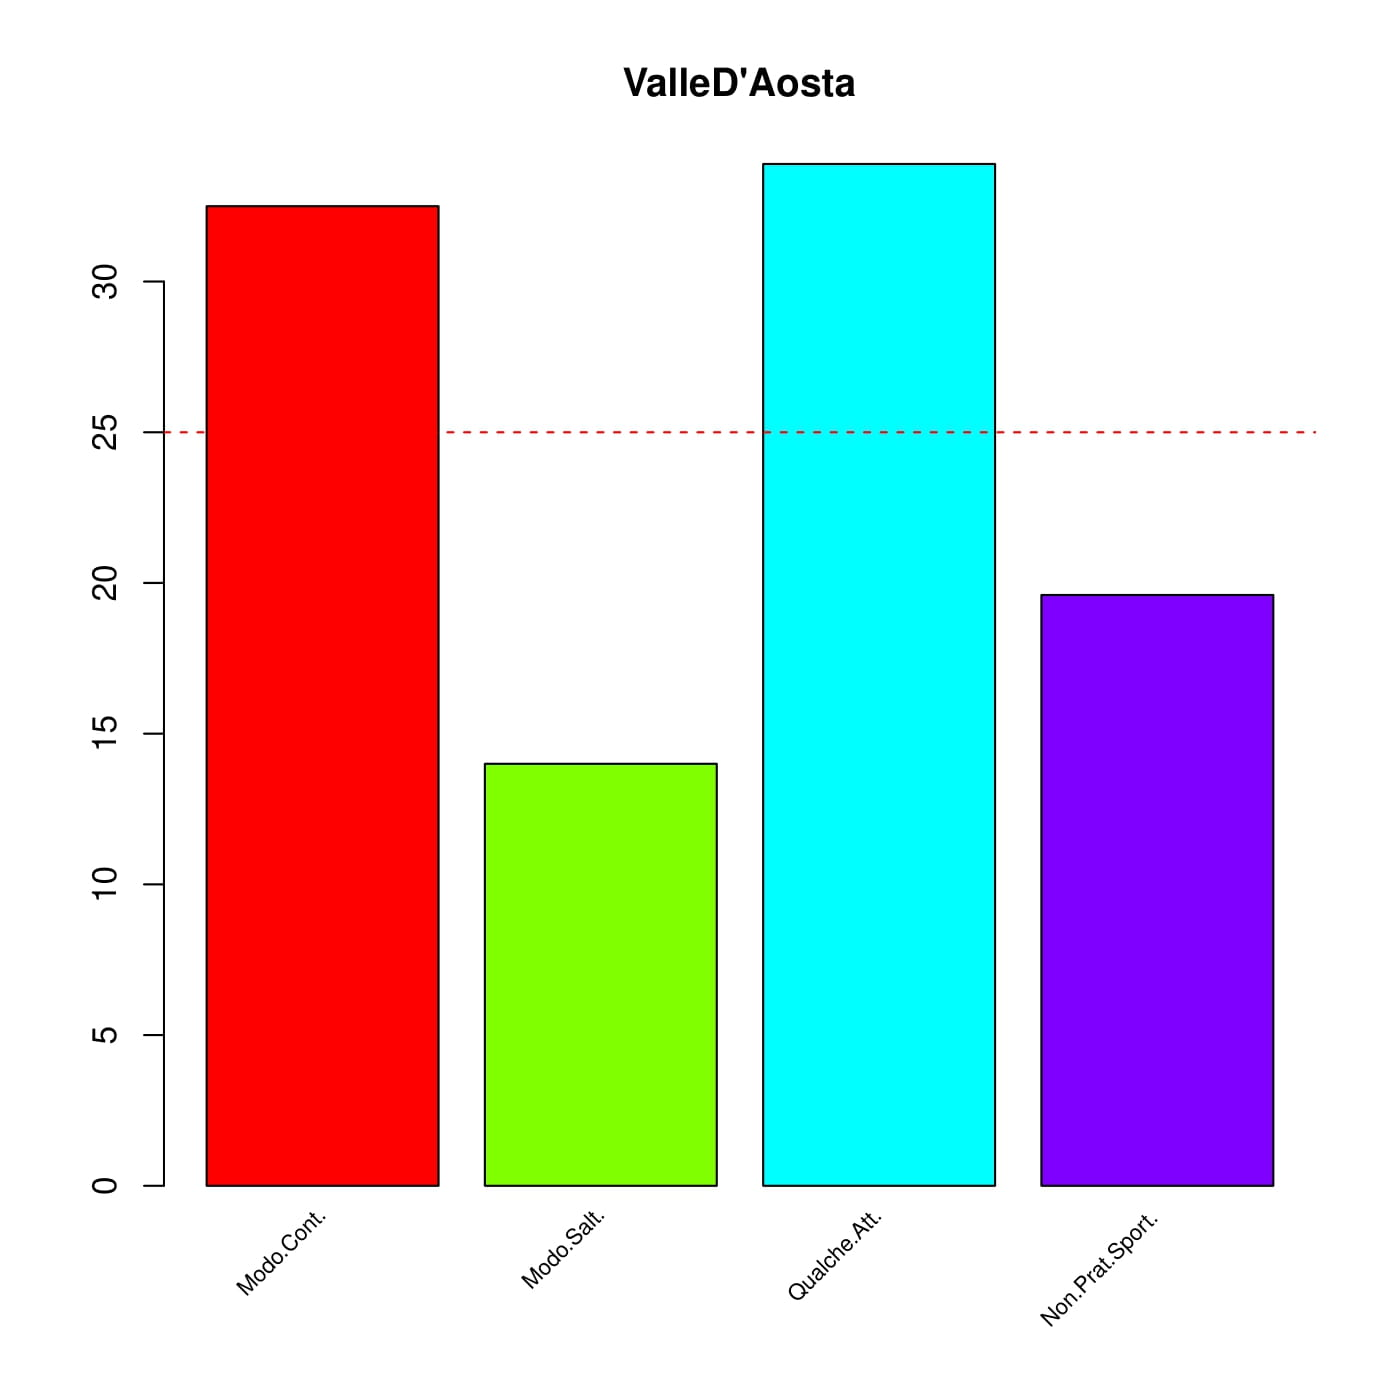
\includegraphics[height=8cm]{ProgettoSAD/capitoli/images/barre_regioni/barre_valledaosta.jpg}}
        \qquad
\end{figure}

\begin{figure}[!htbp]
    \centering
        \subfloat{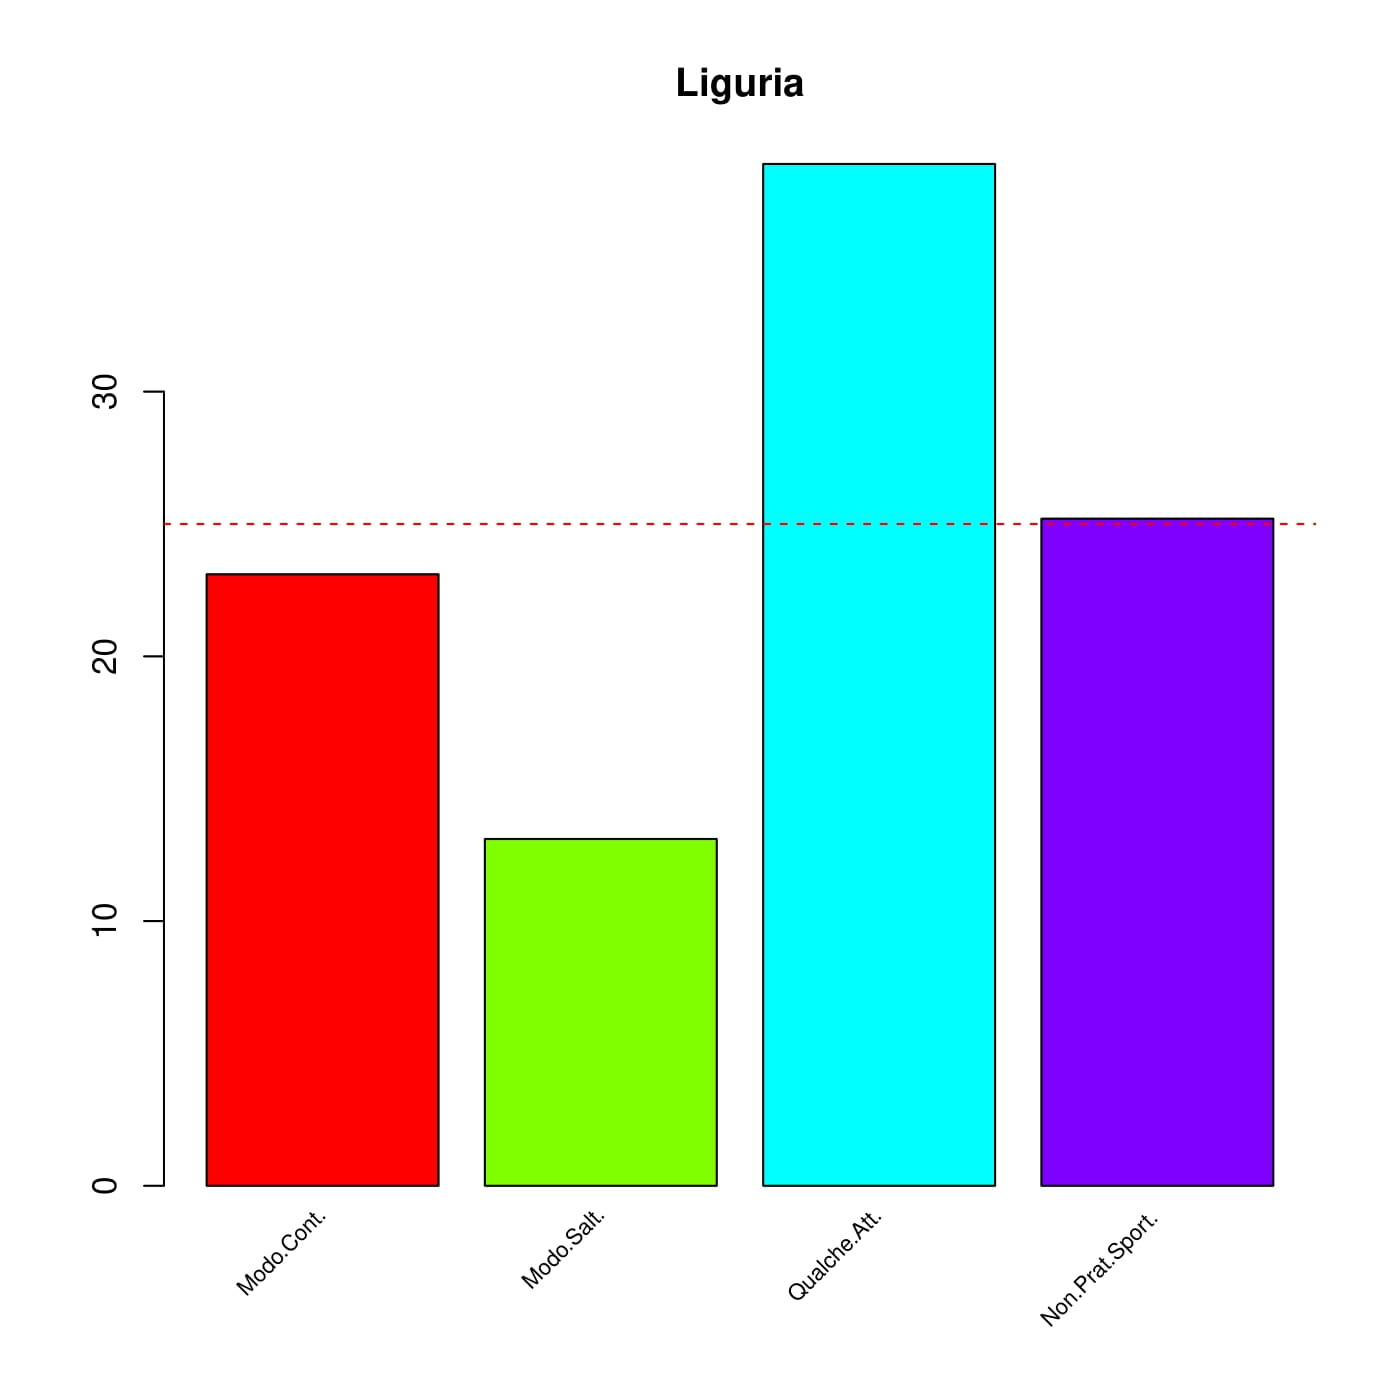
\includegraphics[height=8cm]{ProgettoSAD/capitoli/images/barre_regioni/barre_liguria.jpg}}
        \qquad
        \subfloat{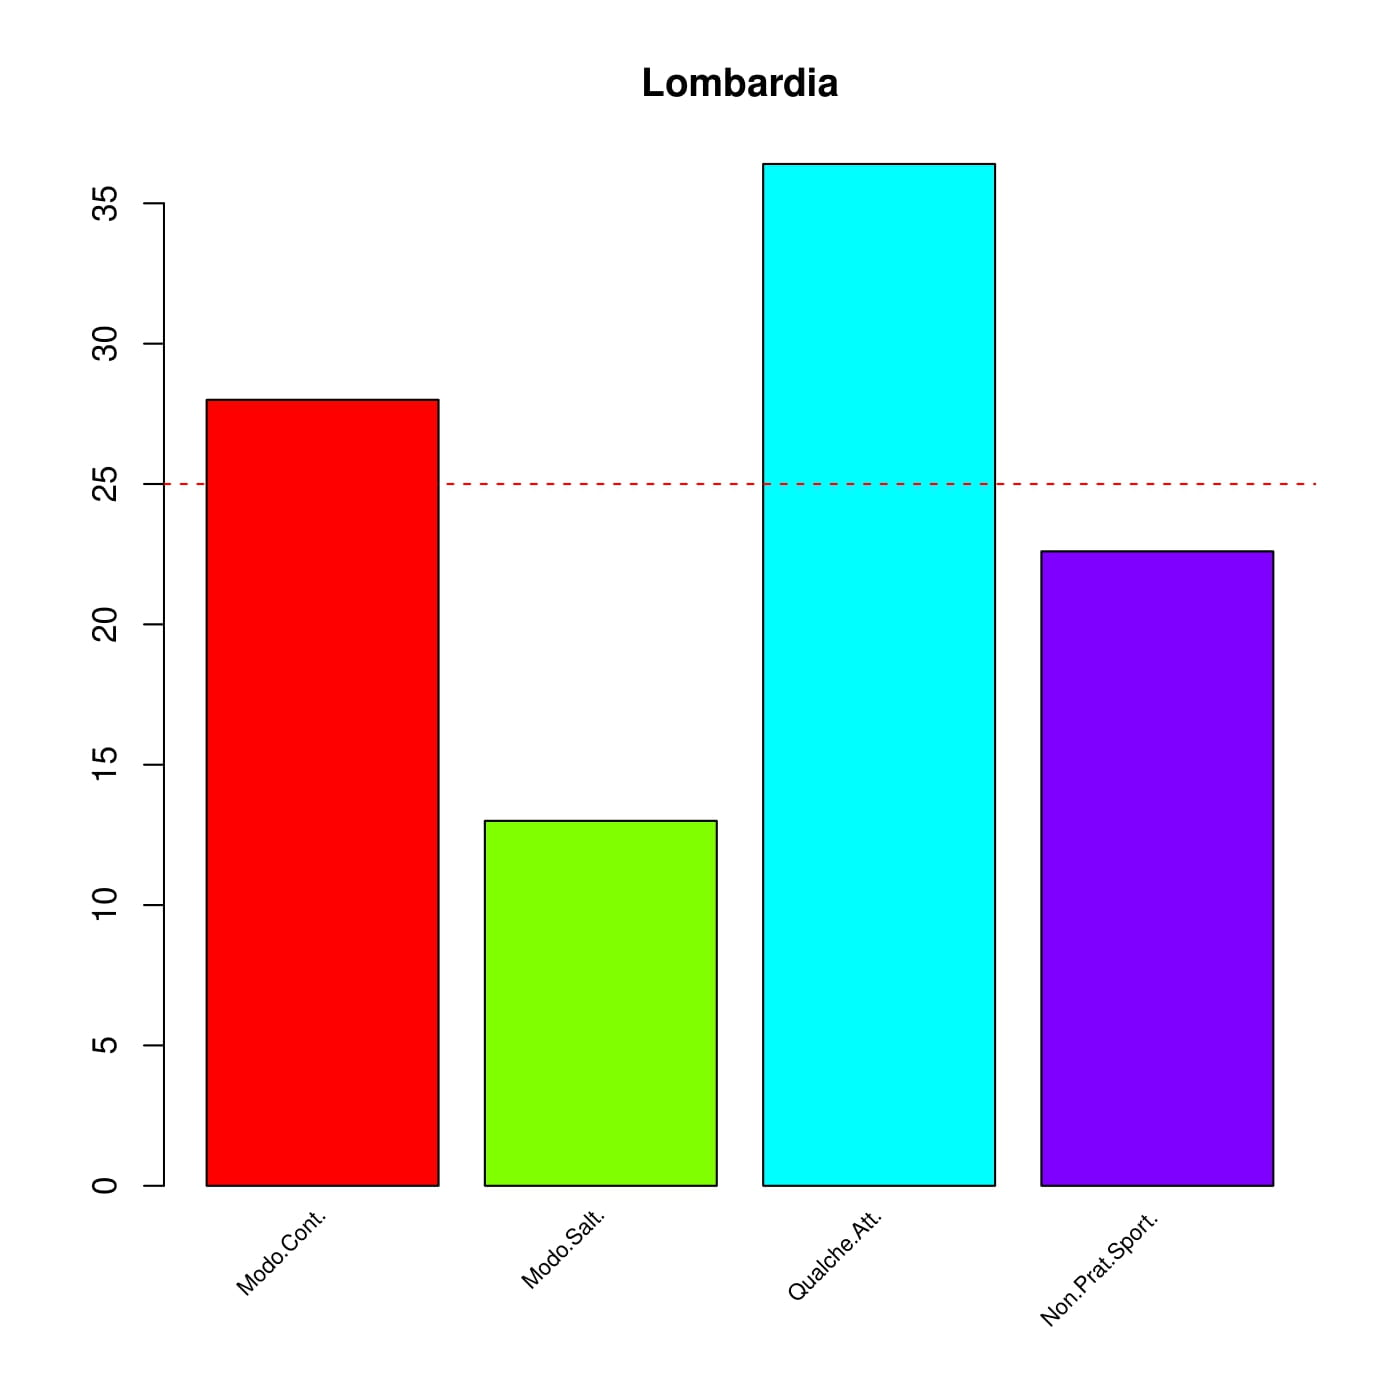
\includegraphics[height=8cm]{ProgettoSAD/capitoli/images/barre_regioni/barre_lombardia.jpg}}
        \qquad
\end{figure}

\begin{figure}[!htbp]
    \centering
        \subfloat{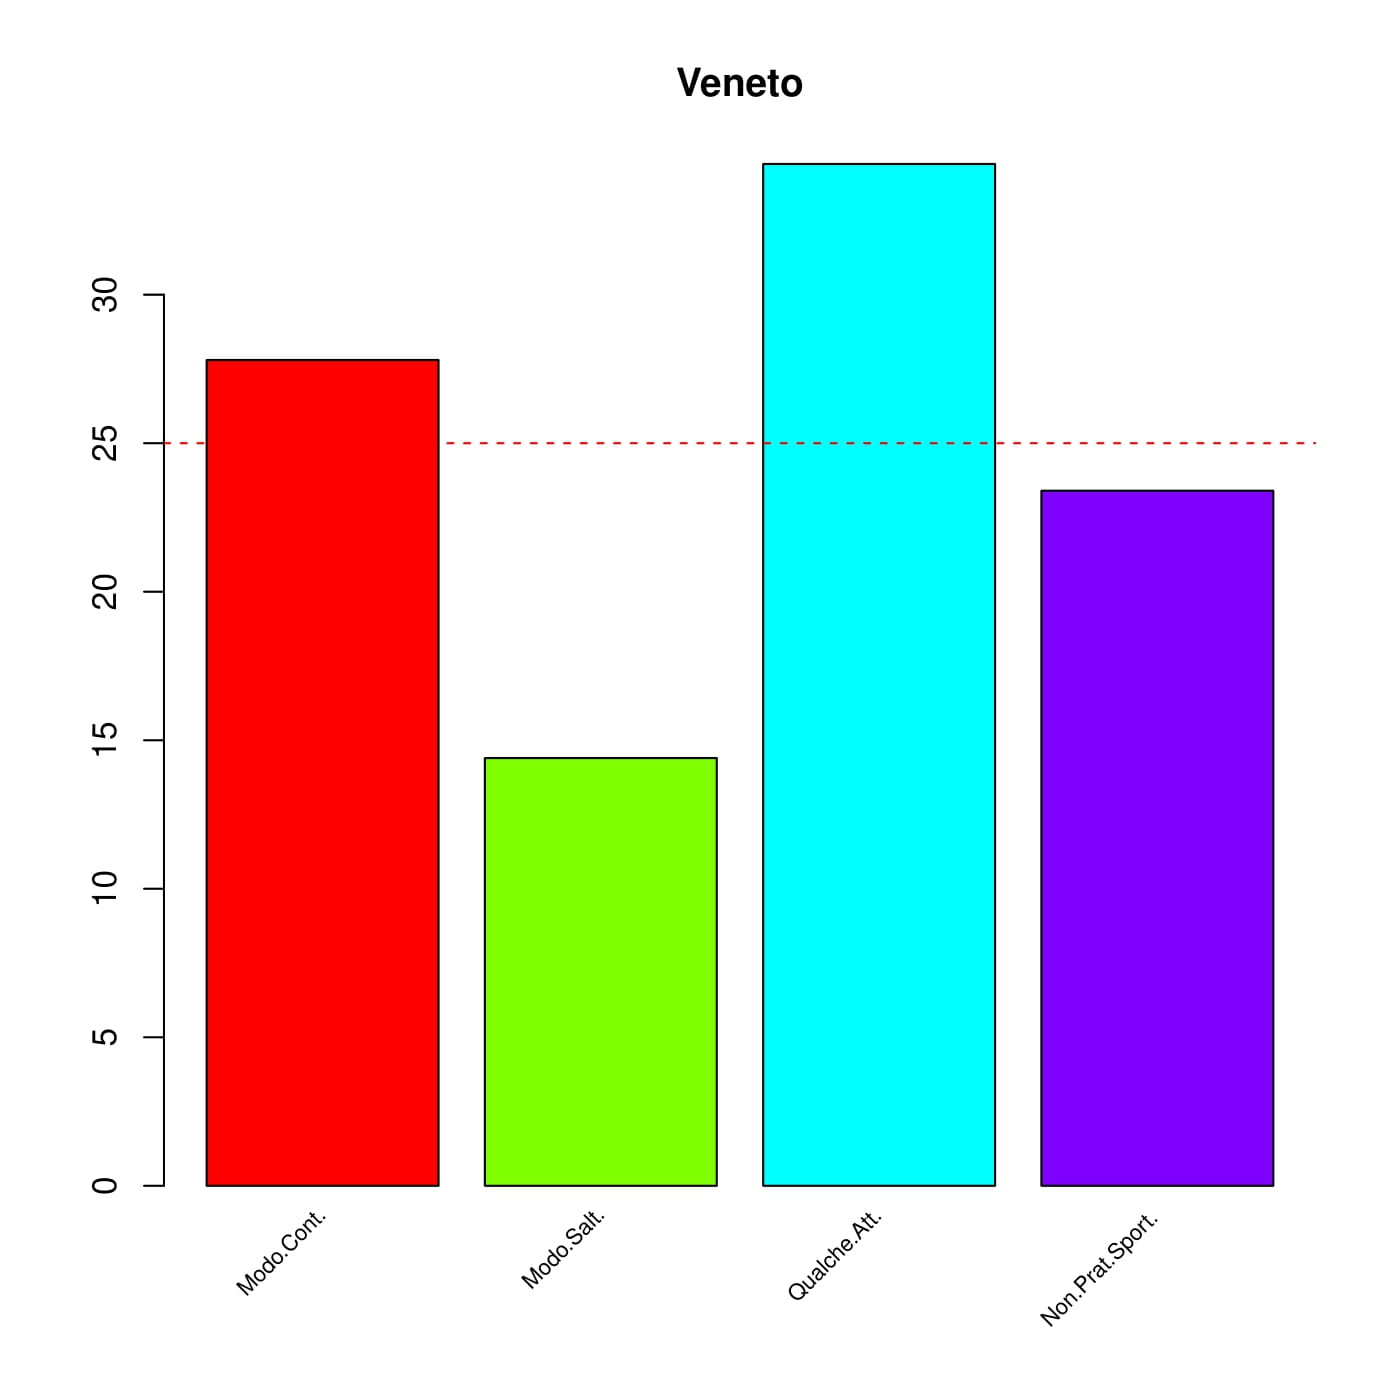
\includegraphics[height=8cm]{ProgettoSAD/capitoli/images/barre_regioni/barre_veneto.jpg}}
        \qquad
        \subfloat{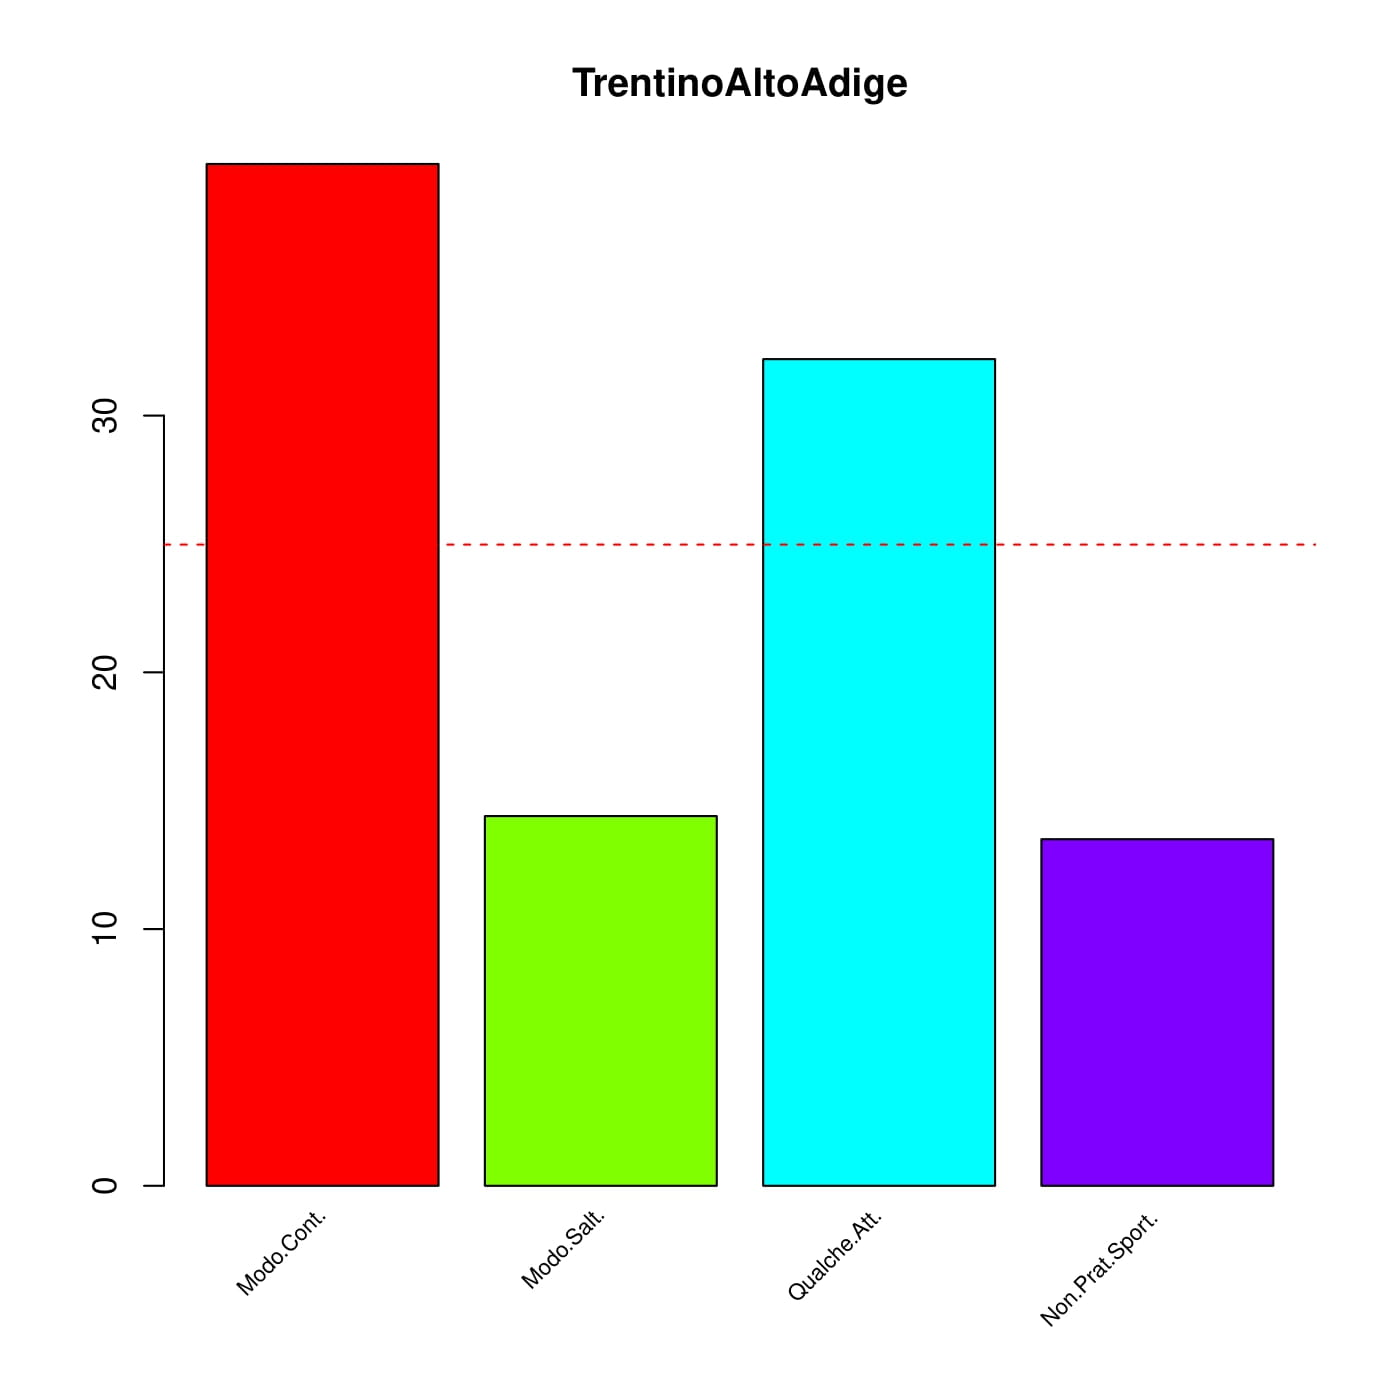
\includegraphics[height=8cm]{ProgettoSAD/capitoli/images/barre_regioni/barre_trentino.jpg}}
        \qquad
\end{figure}

\begin{figure}[!htbp]
    \centering
        \subfloat{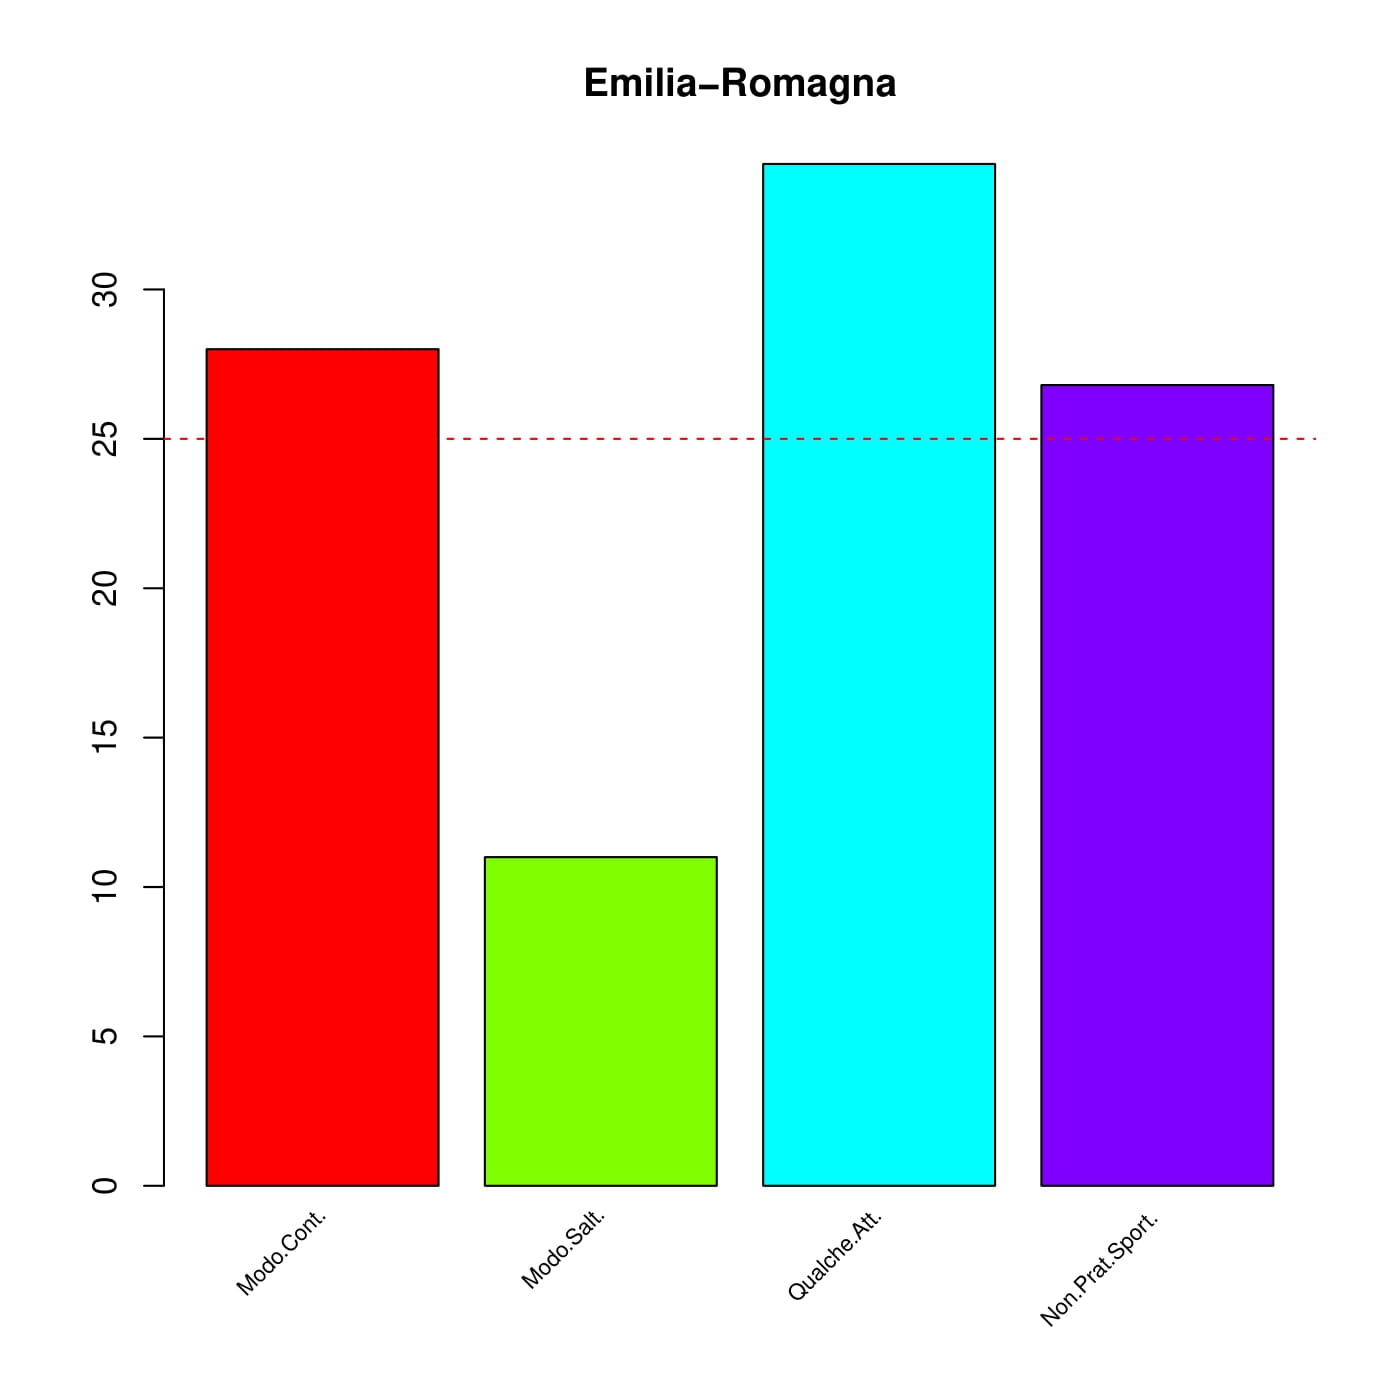
\includegraphics[height=8cm]{ProgettoSAD/capitoli/images/barre_regioni/barre_emilia.jpg}}
        \qquad
        \subfloat{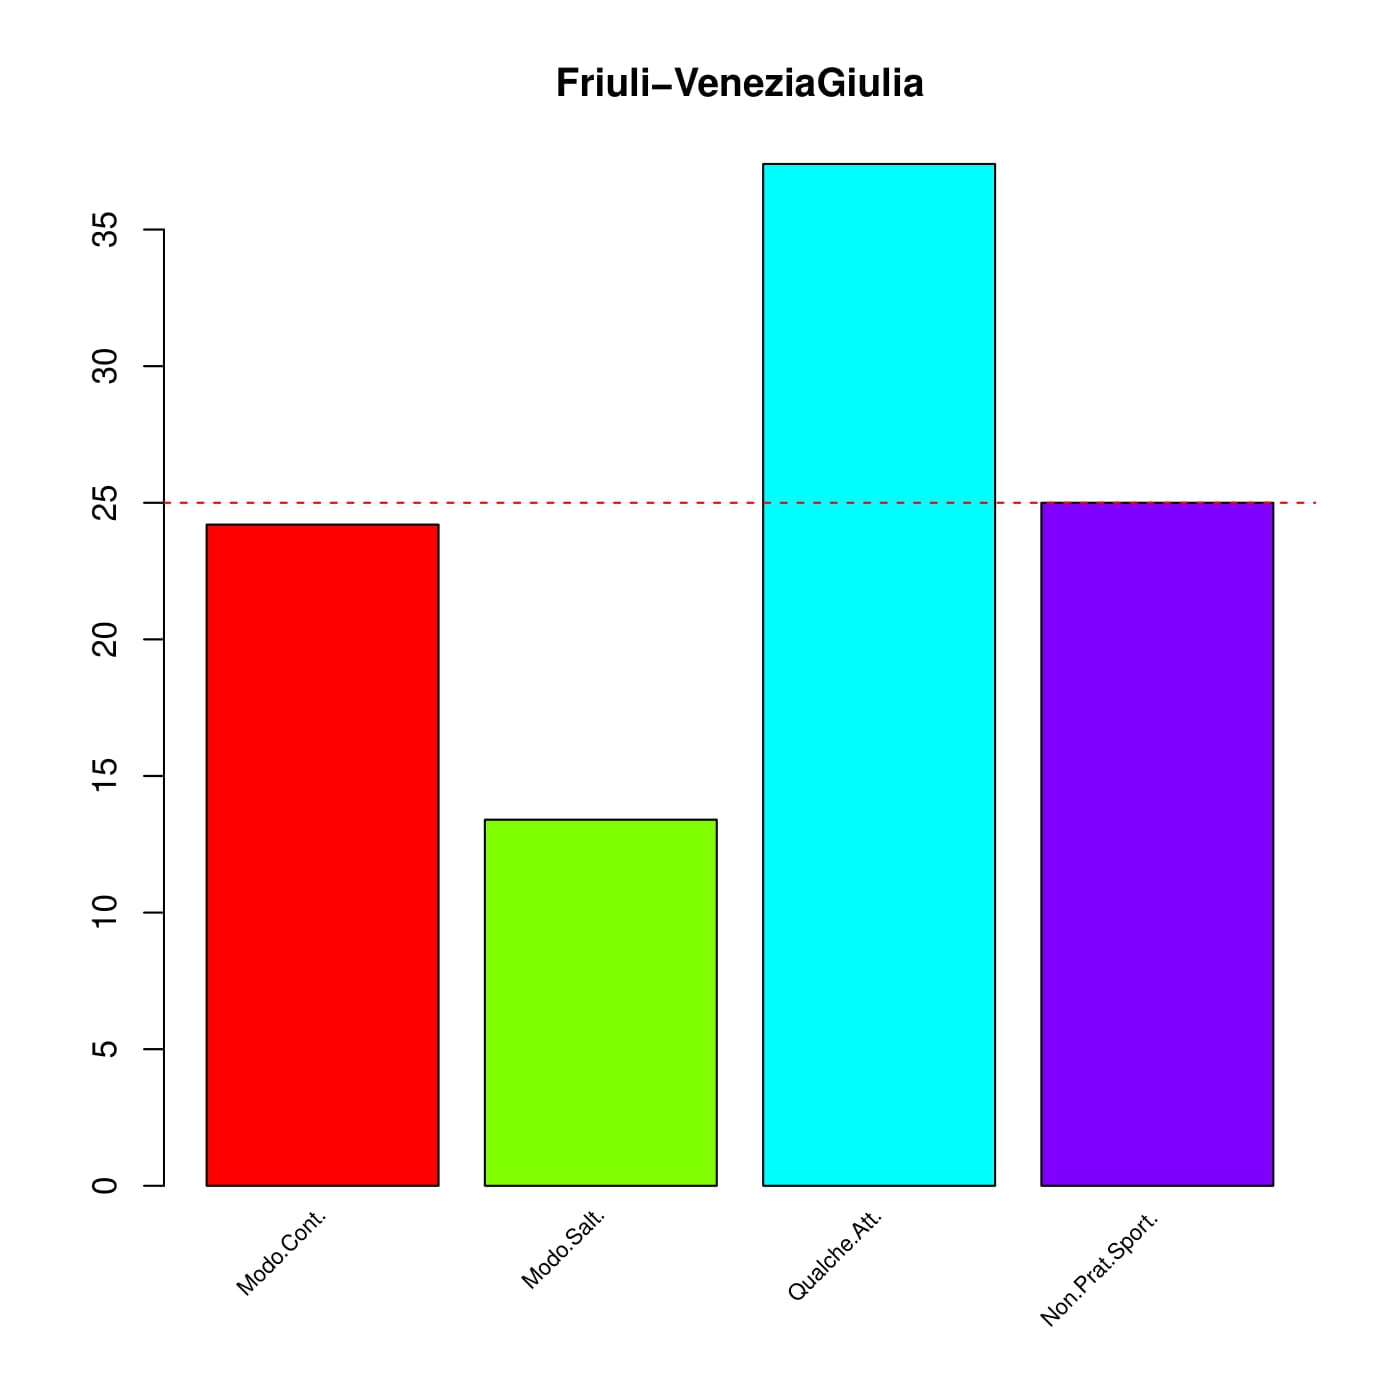
\includegraphics[height=8cm]{ProgettoSAD/capitoli/images/barre_regioni/barre_friuli.jpg}}
        \qquad
\end{figure}

\begin{figure}[!htbp]
    \centering
        \subfloat{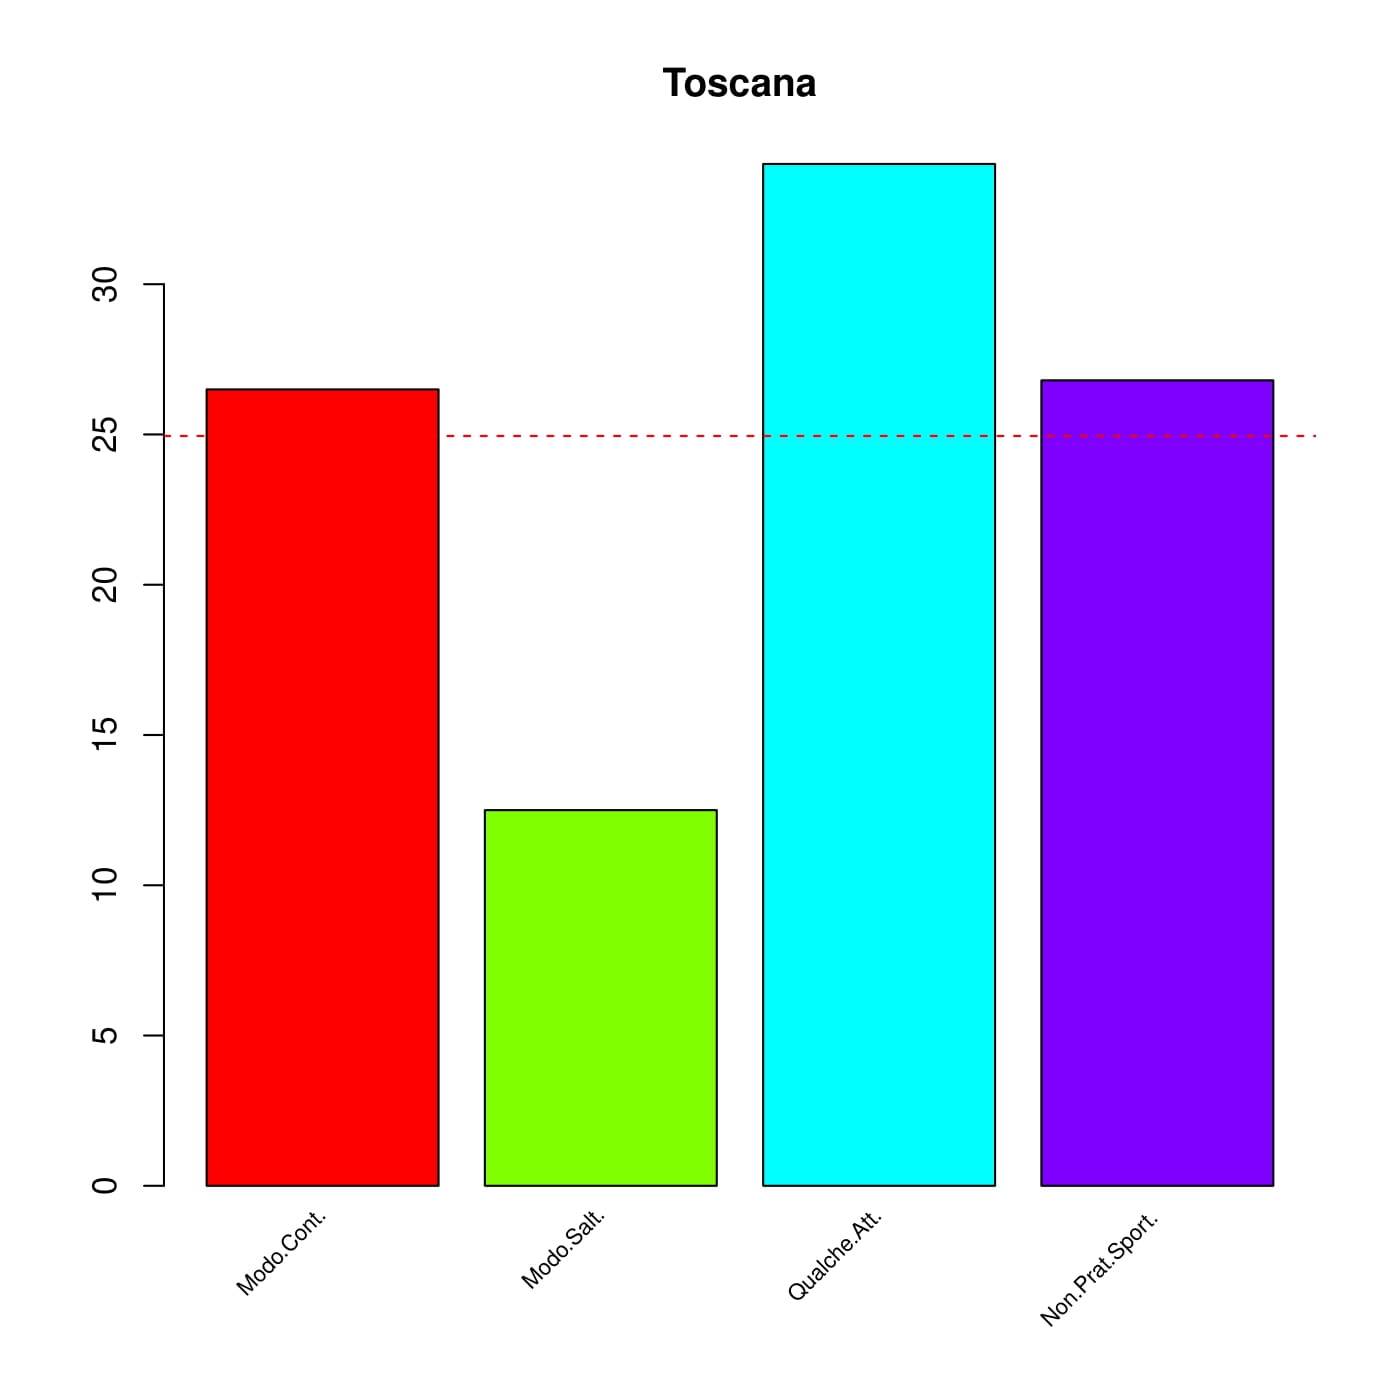
\includegraphics[height=8cm]{ProgettoSAD/capitoli/images/barre_regioni/barre_toscana.jpg}}
        \qquad
        \subfloat{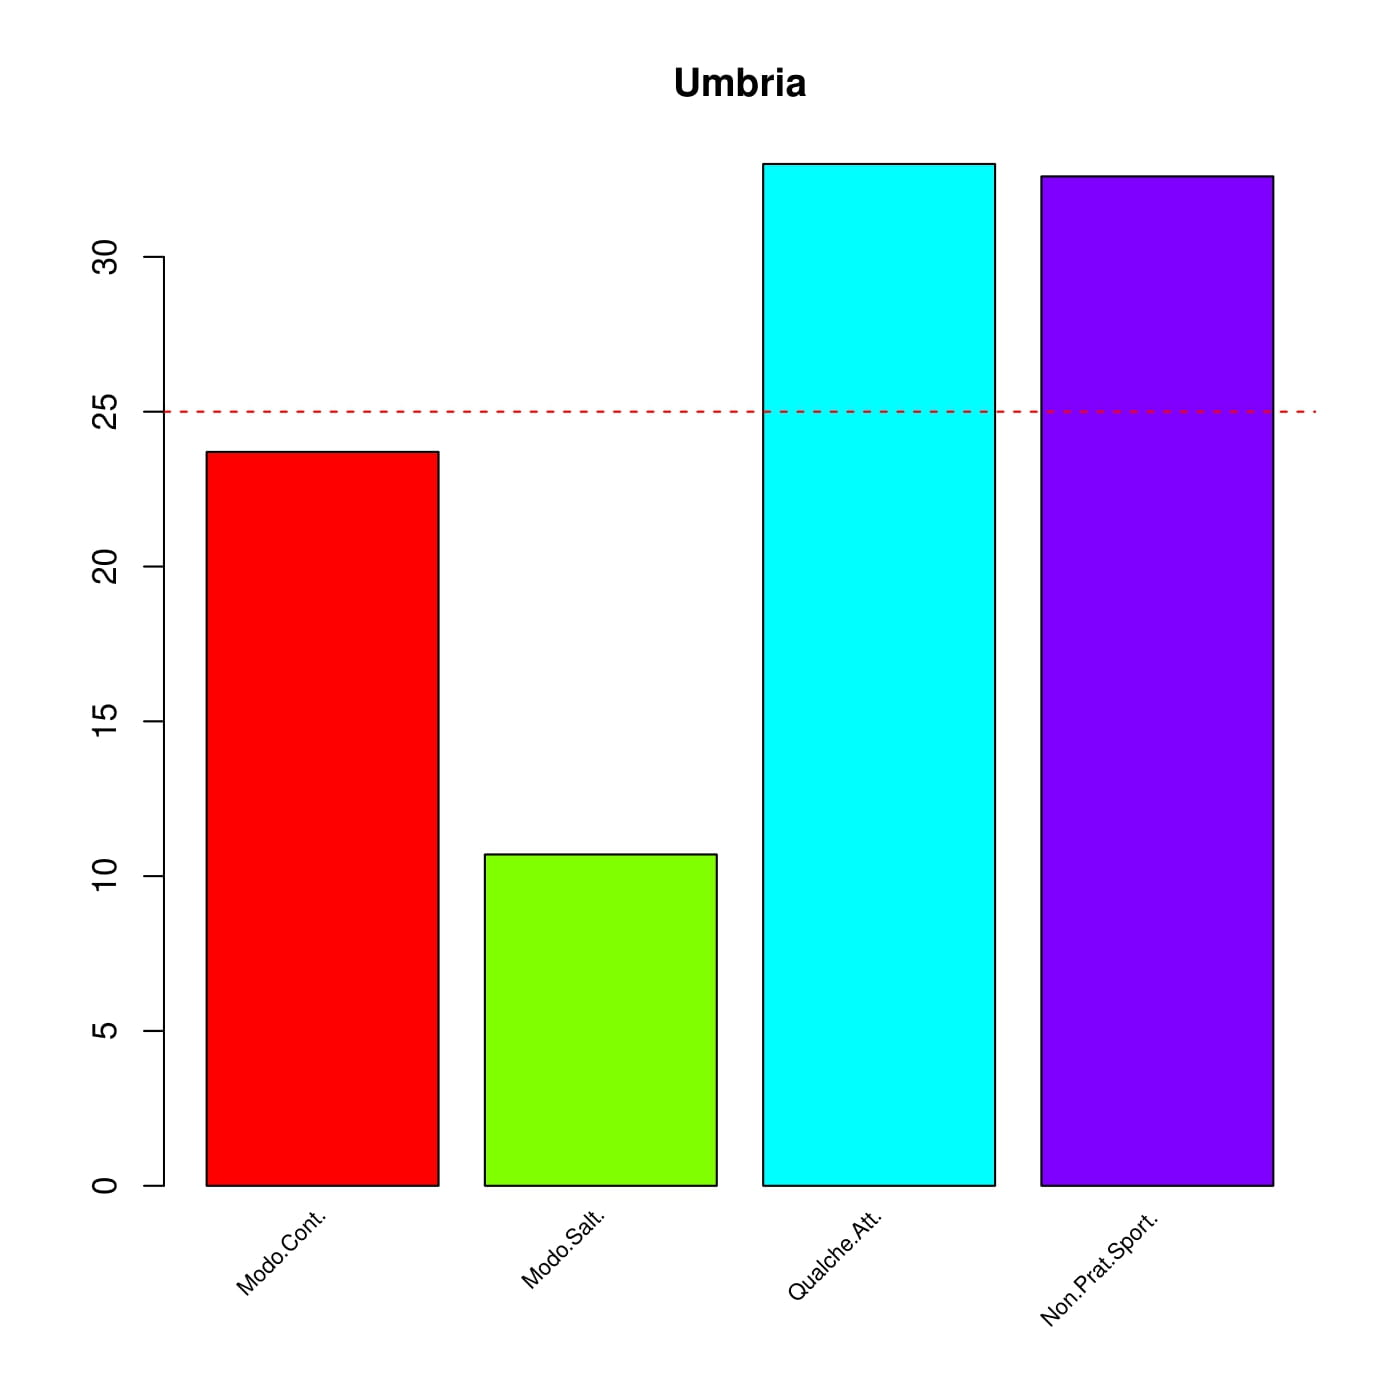
\includegraphics[height=8cm]{ProgettoSAD/capitoli/images/barre_regioni/barre_umbria.jpg}}
        \qquad
\end{figure}

\begin{figure}[!htbp]
    \centering
        \subfloat{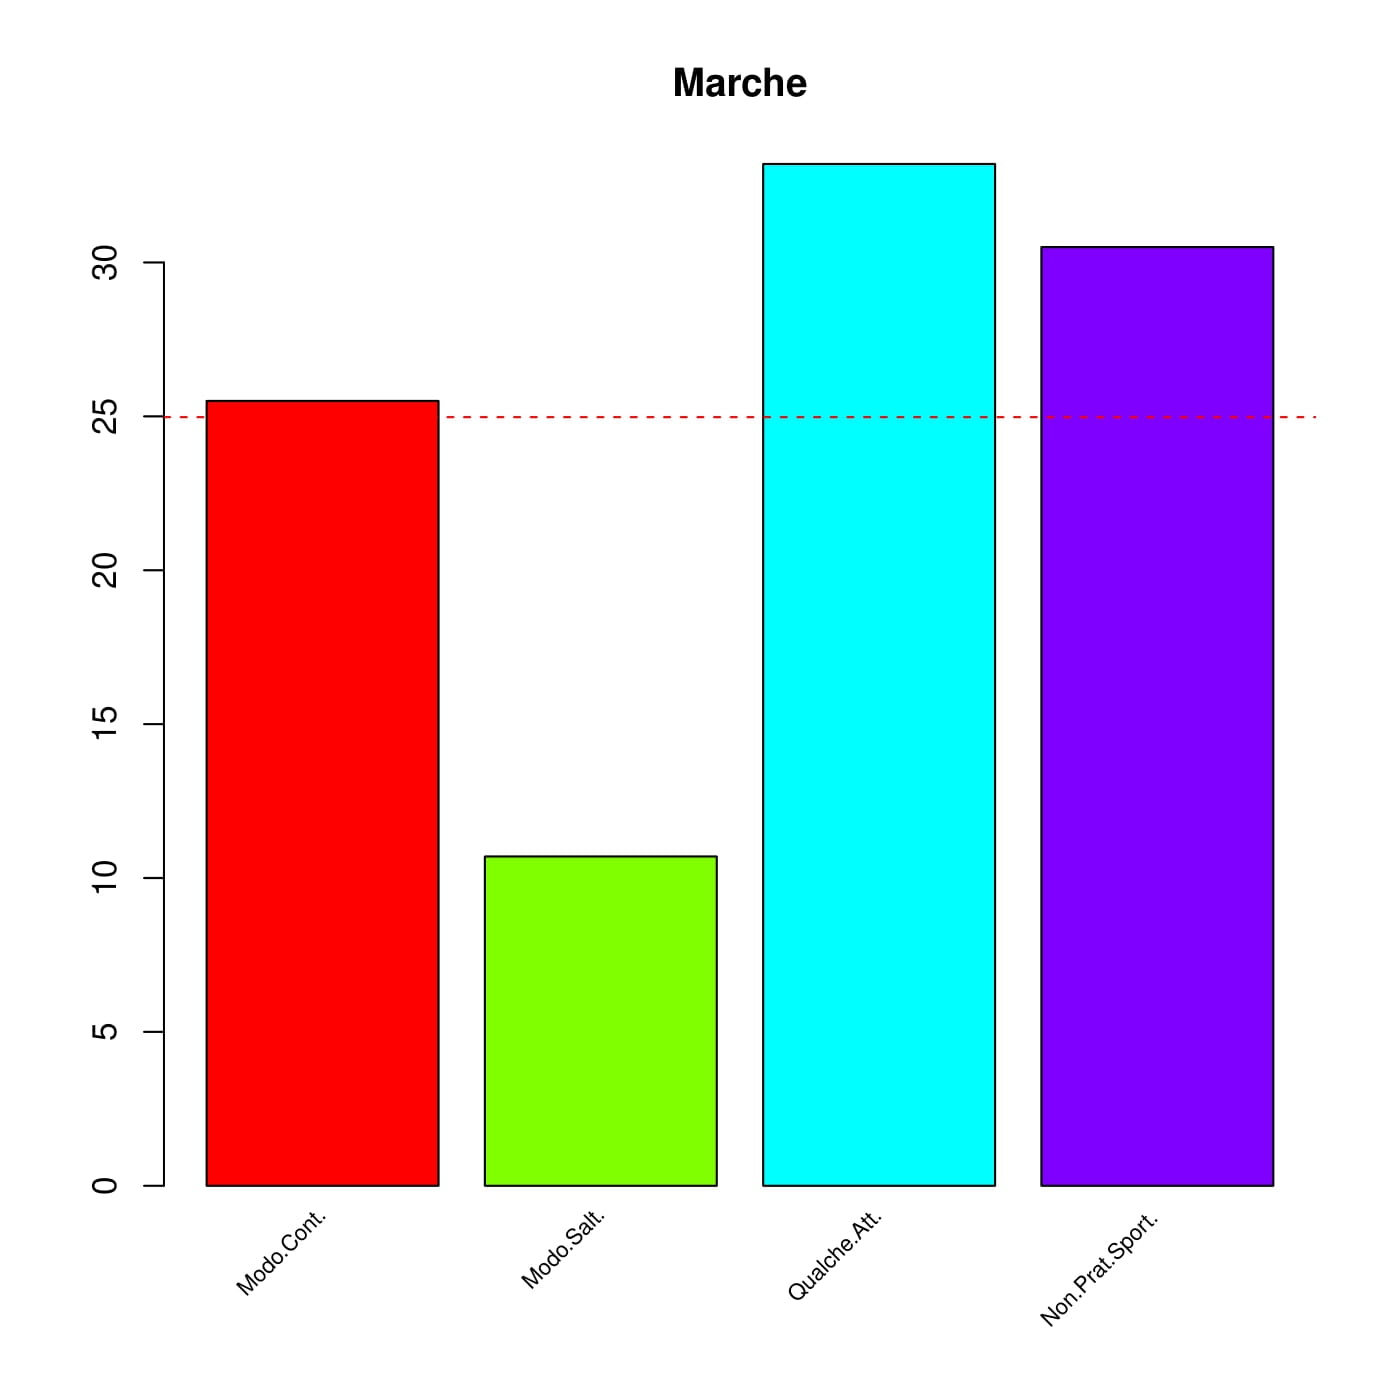
\includegraphics[height=8cm]{ProgettoSAD/capitoli/images/barre_regioni/barre_marche.jpg}}
        \qquad
        \subfloat{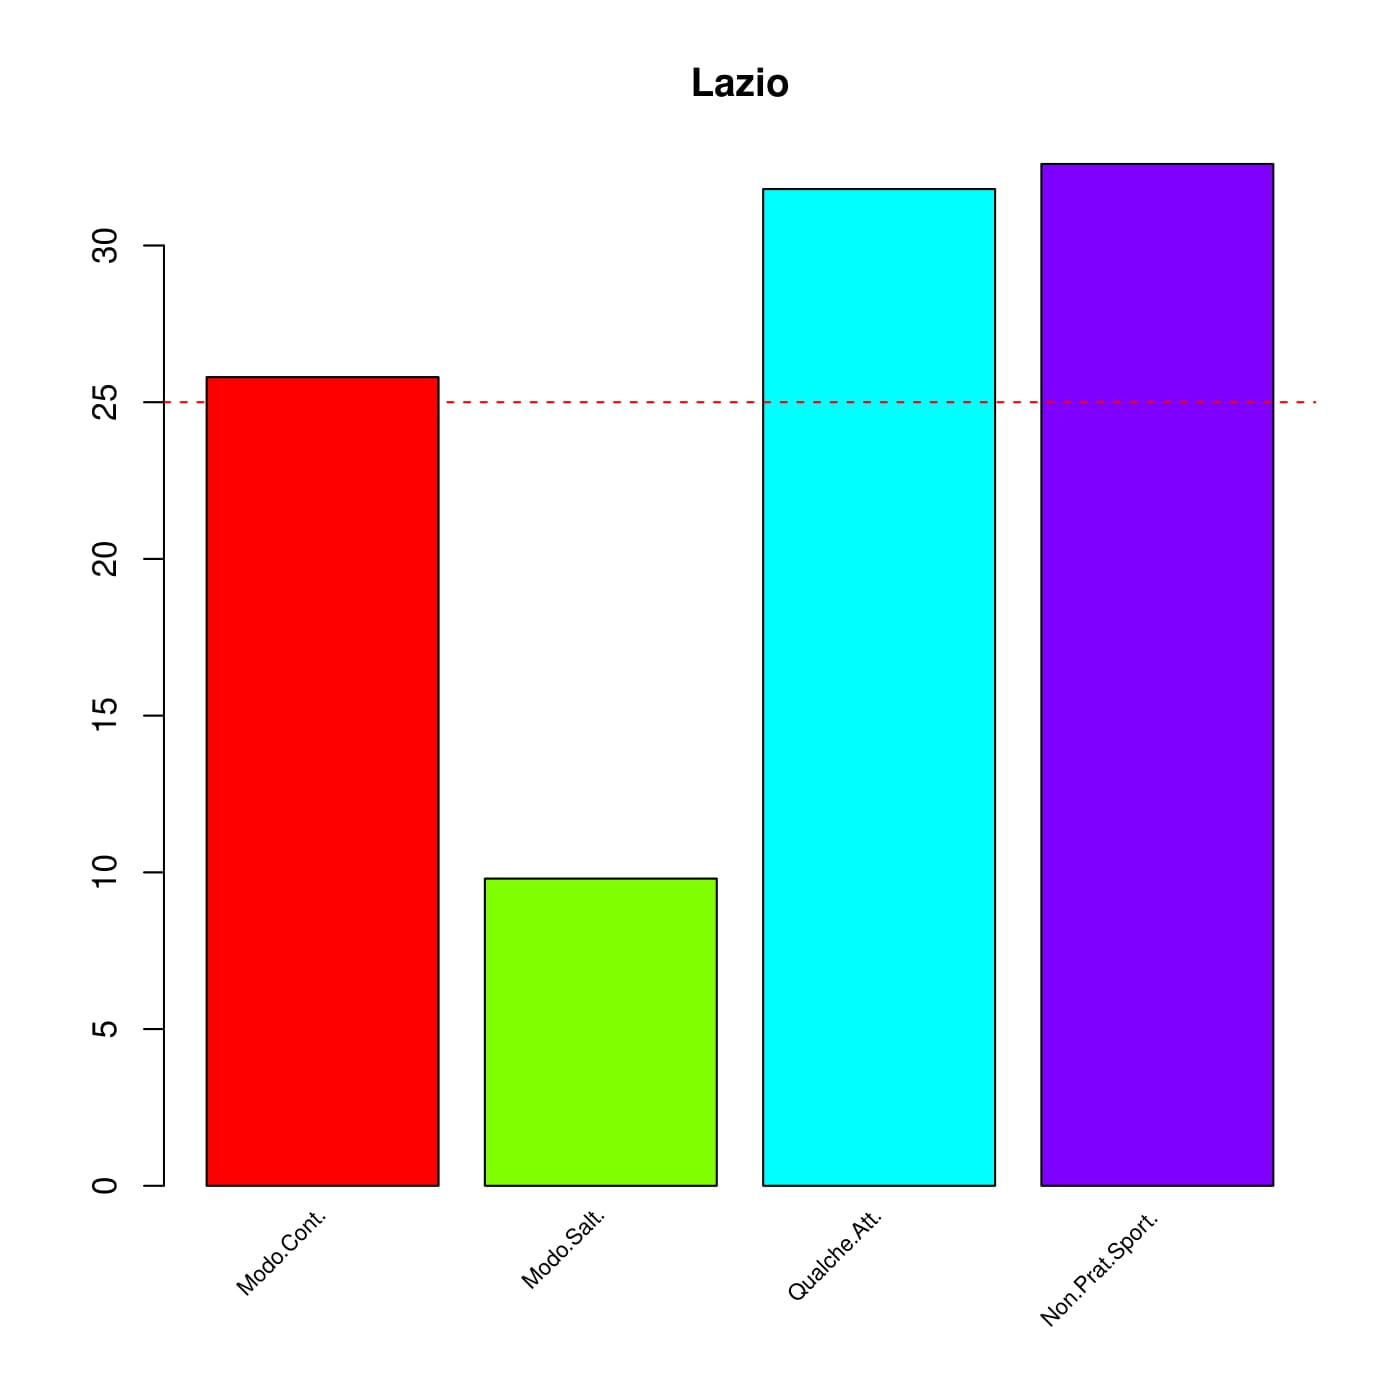
\includegraphics[height=8cm]{ProgettoSAD/capitoli/images/barre_regioni/barre_lazio.jpg}}
        \qquad
\end{figure}

\begin{figure}[!htbp]
    \centering
        \subfloat{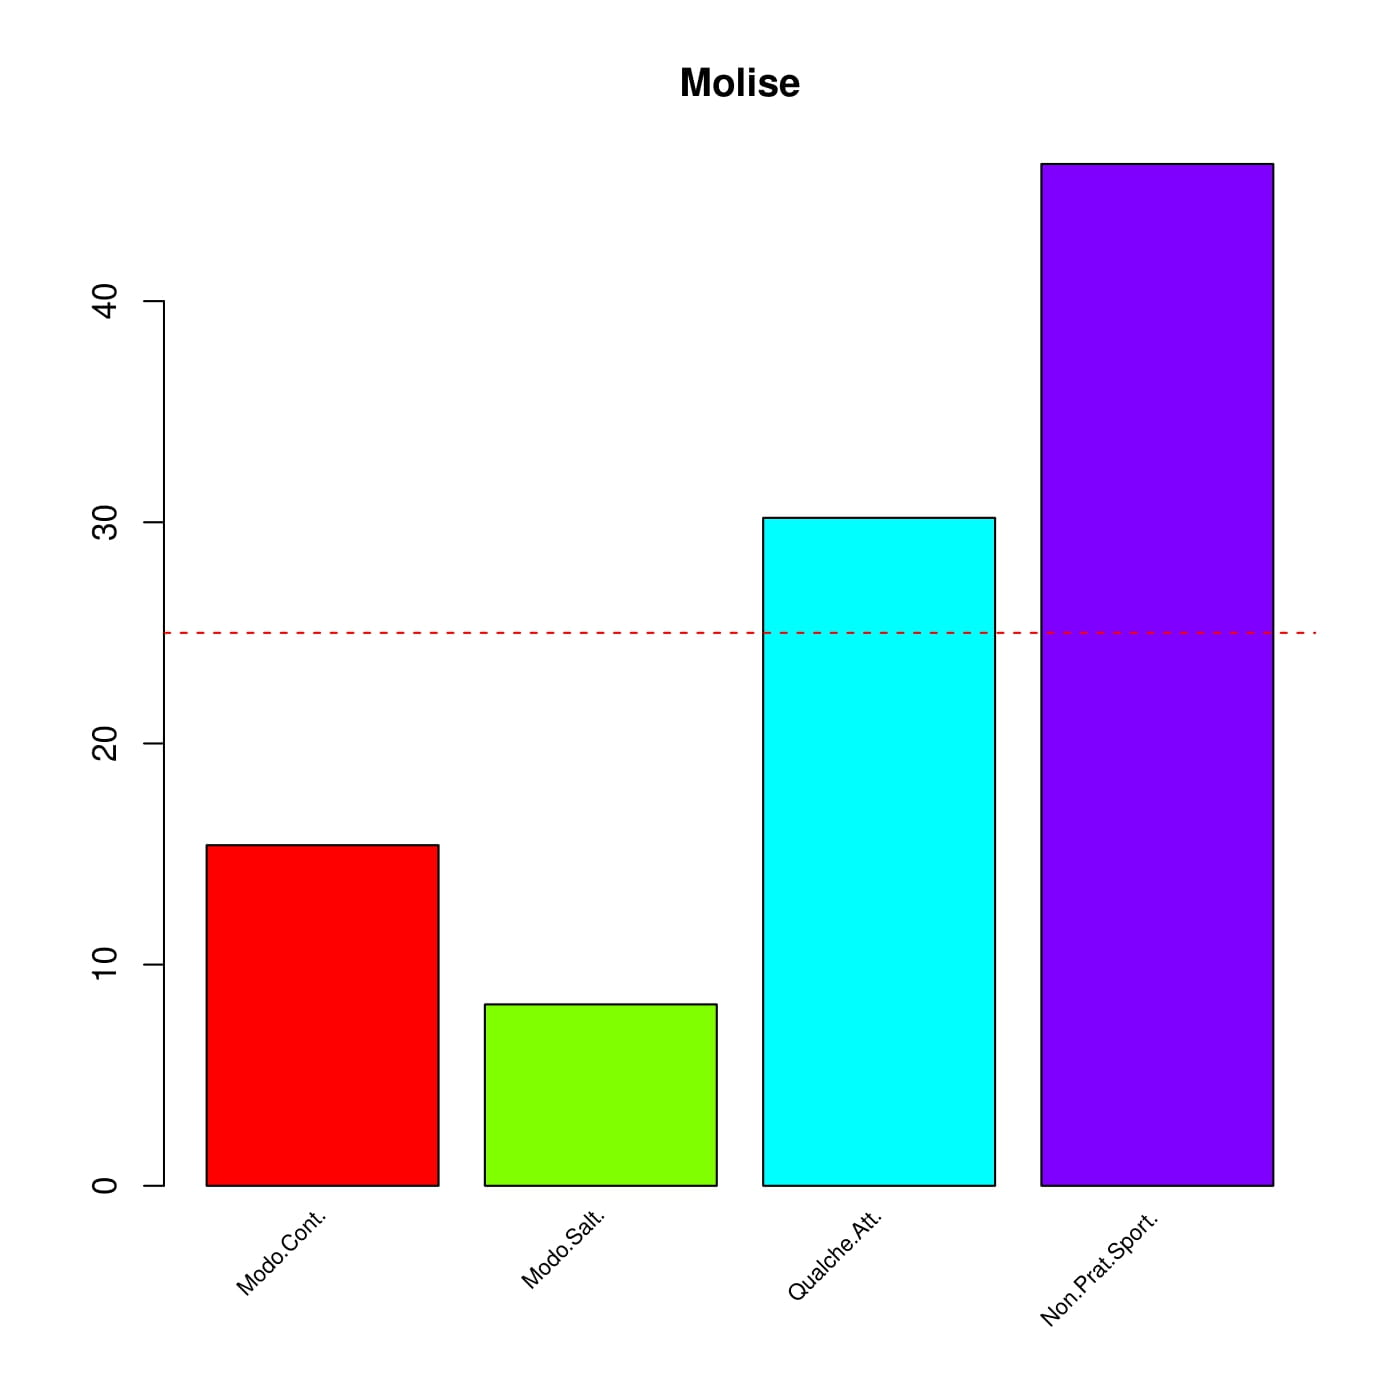
\includegraphics[height=8cm]{ProgettoSAD/capitoli/images/barre_regioni/barre_molise.jpg}}
        \qquad
        \subfloat{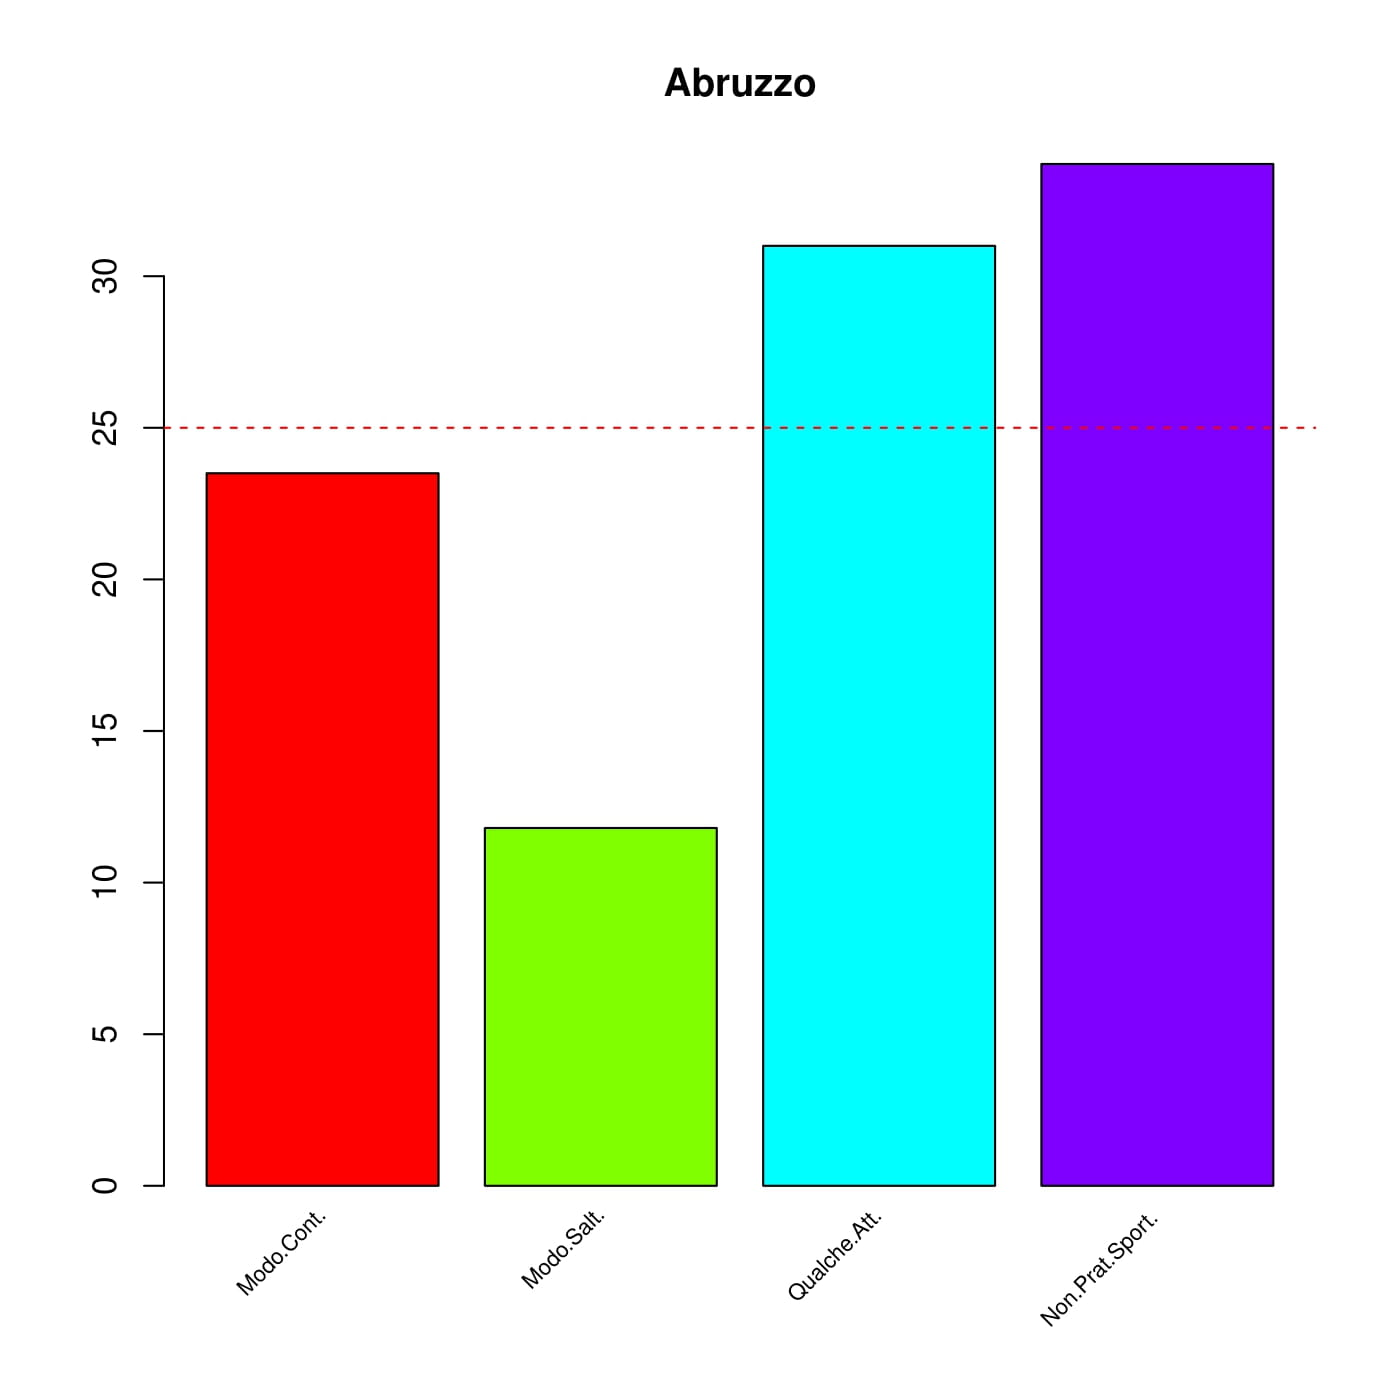
\includegraphics[height=8cm]{ProgettoSAD/capitoli/images/barre_regioni/barre_abruzzo.jpg}}
        \qquad
\end{figure}

\begin{figure}[!htbp]
    \centering
        \subfloat{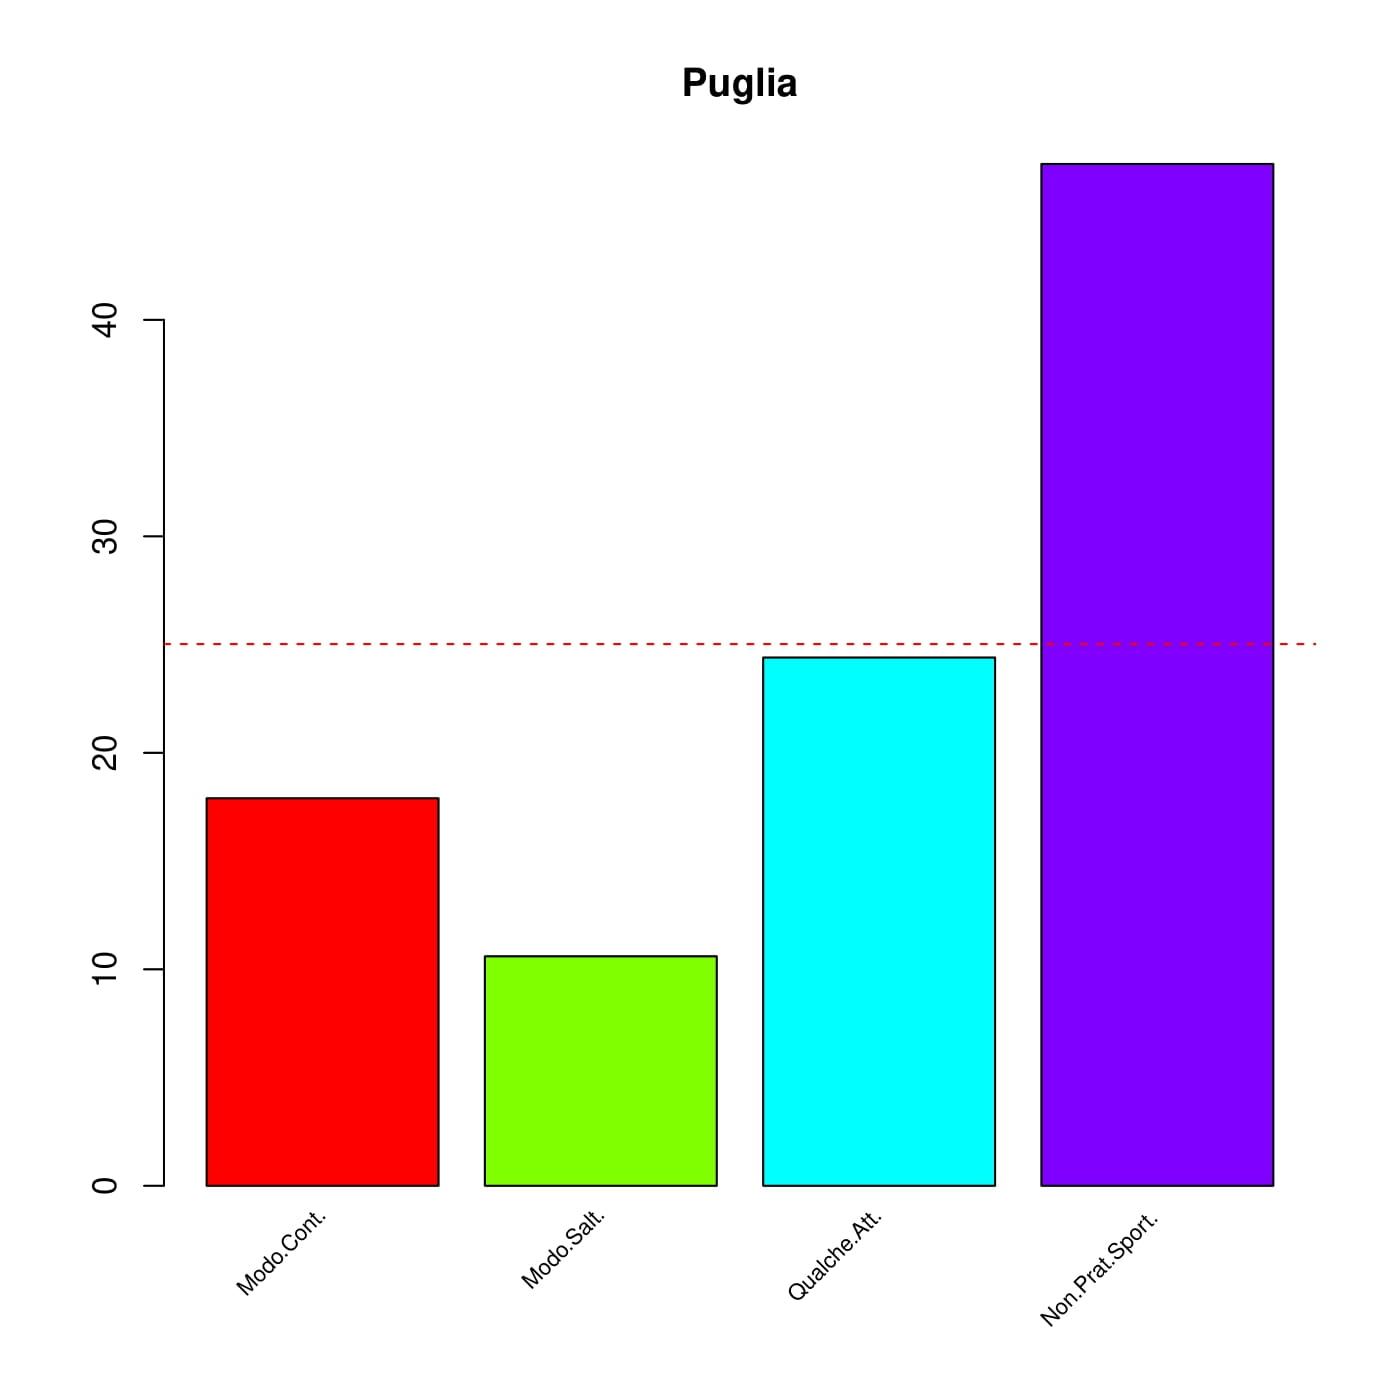
\includegraphics[height=8cm]{ProgettoSAD/capitoli/images/barre_regioni/barre_puglia.jpg}}
        \qquad
        \subfloat{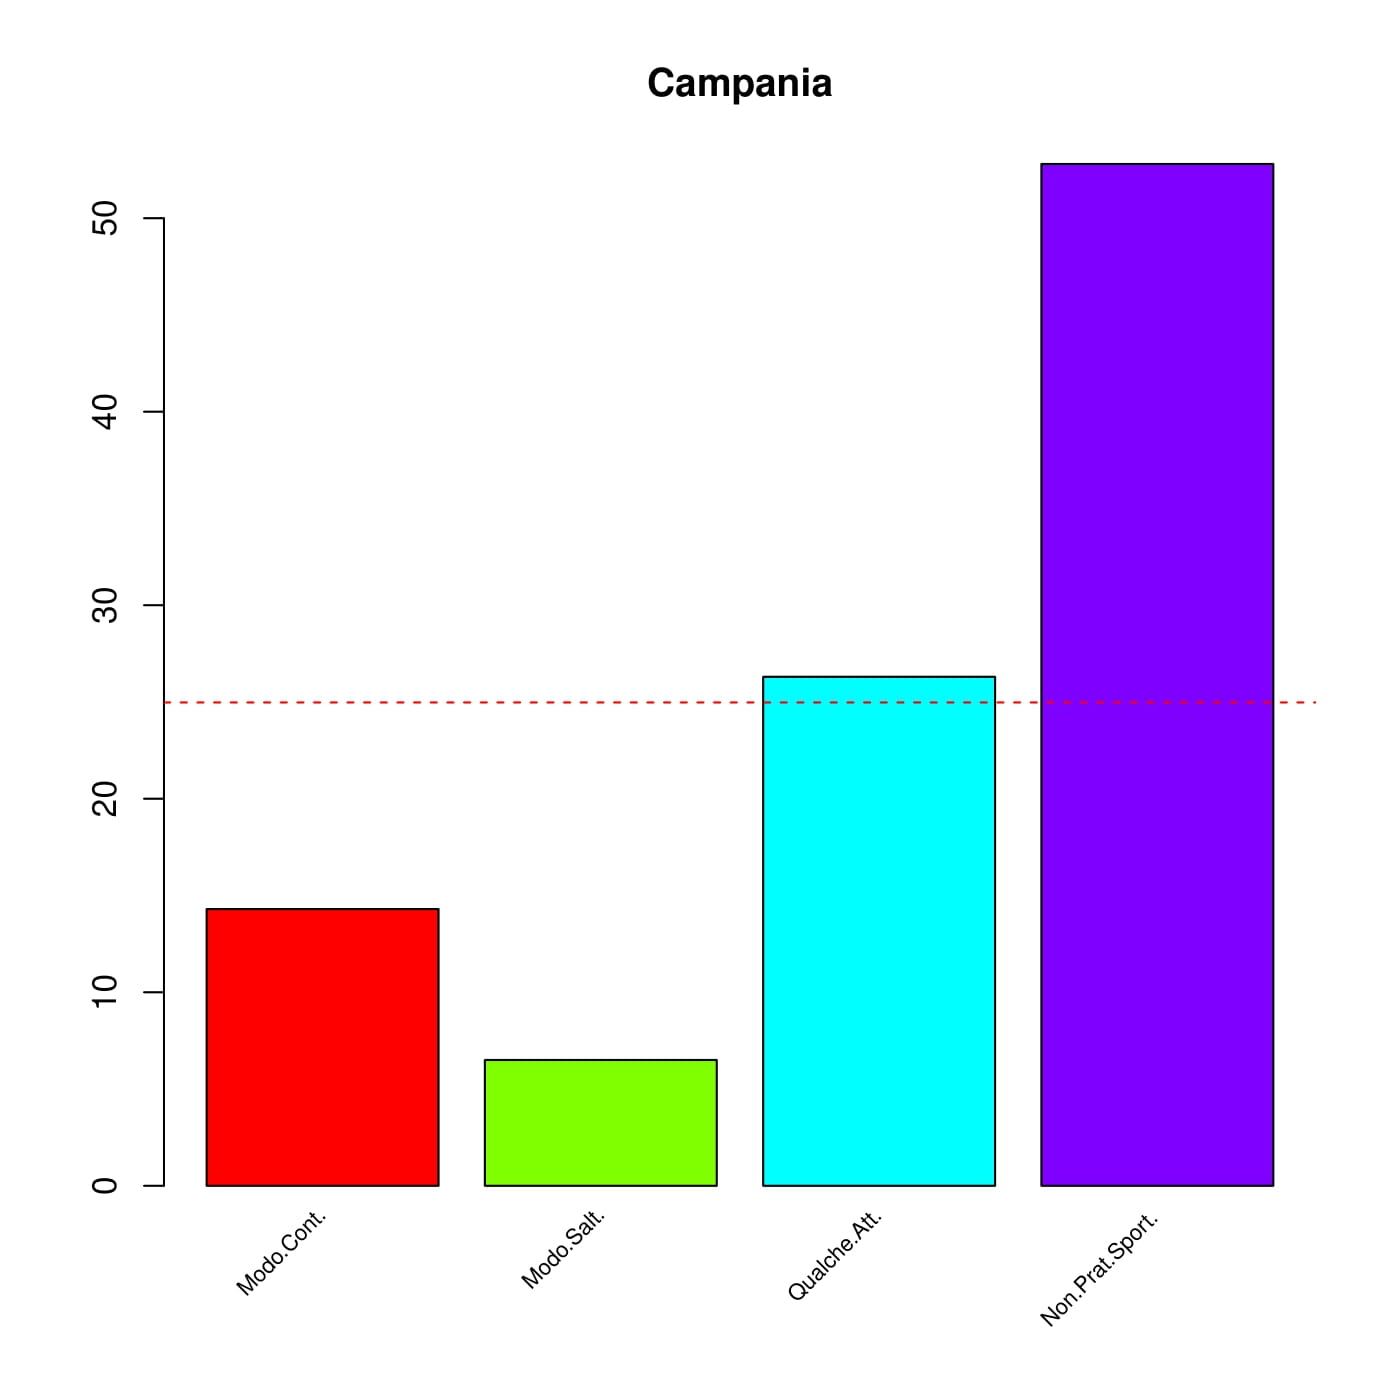
\includegraphics[height=8cm]{ProgettoSAD/capitoli/images/barre_regioni/barre_campania.jpg}}
        \qquad
\end{figure}

\begin{figure}[!htbp]
    \centering
        \subfloat{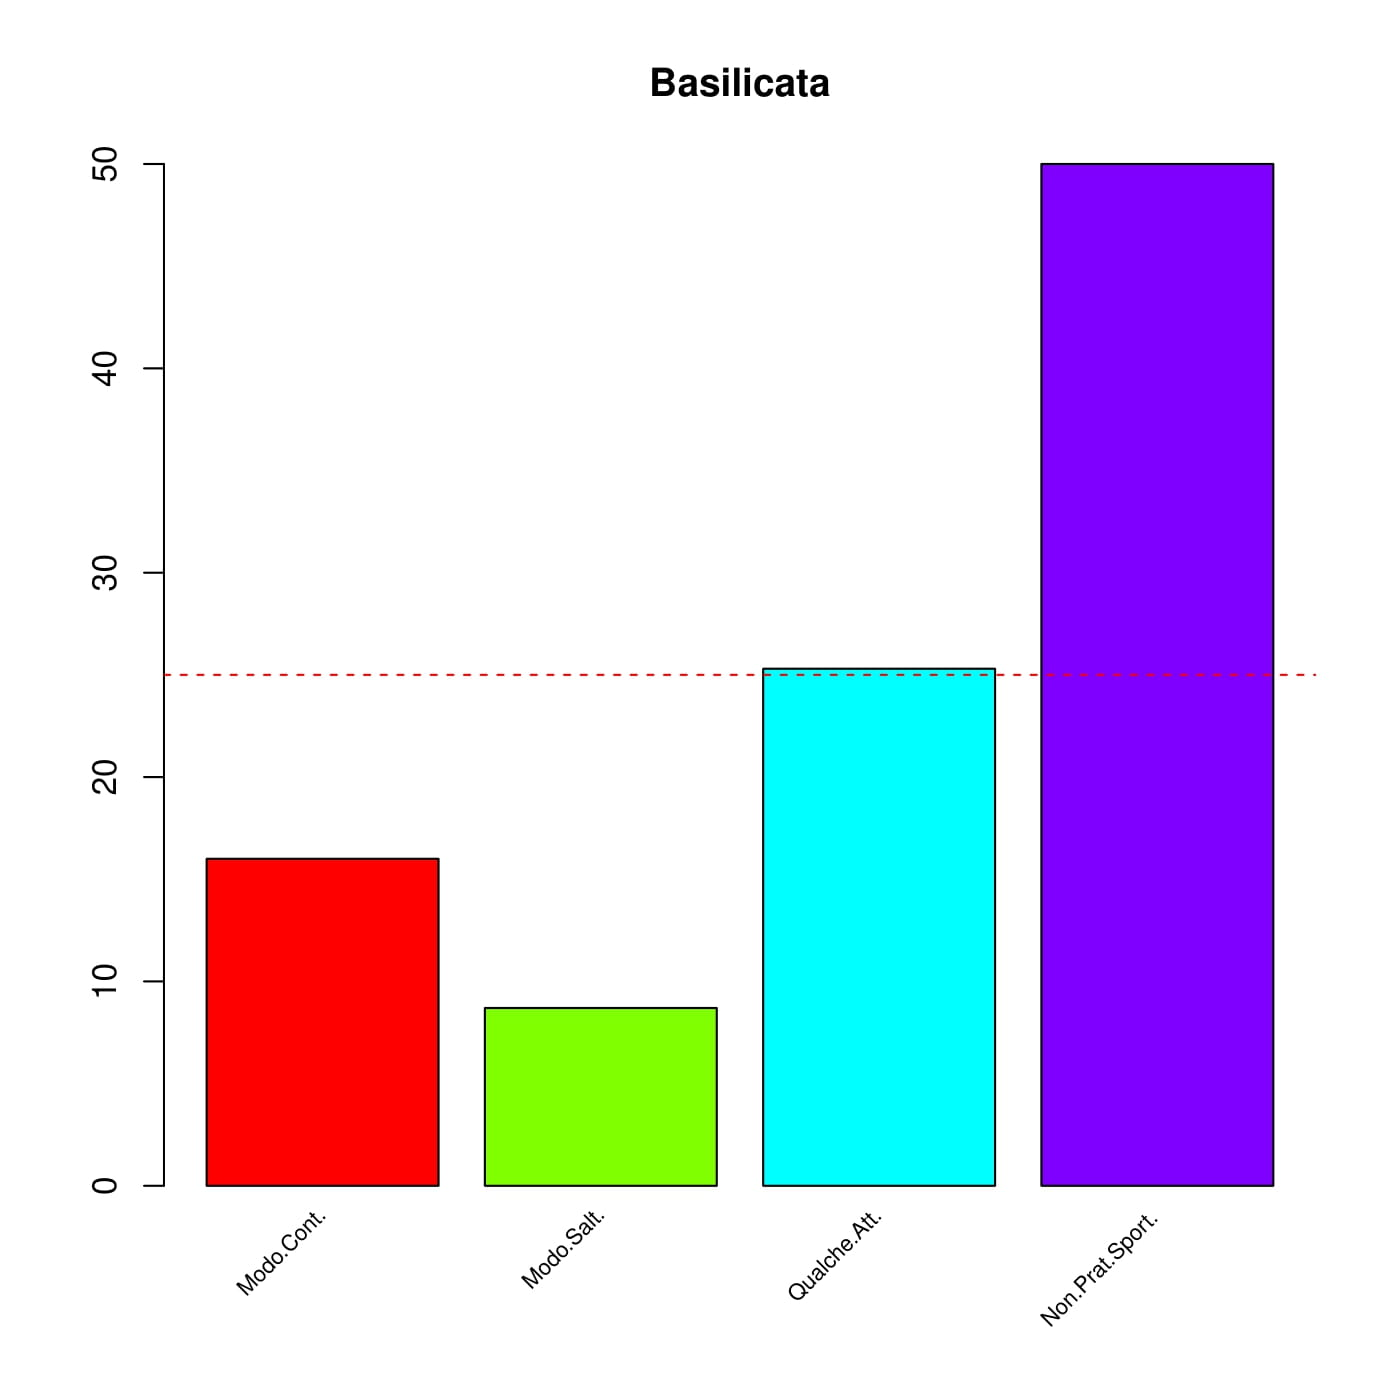
\includegraphics[height=8cm]{ProgettoSAD/capitoli/images/barre_regioni/barre_basilicata.jpg}}
        \qquad
        \subfloat{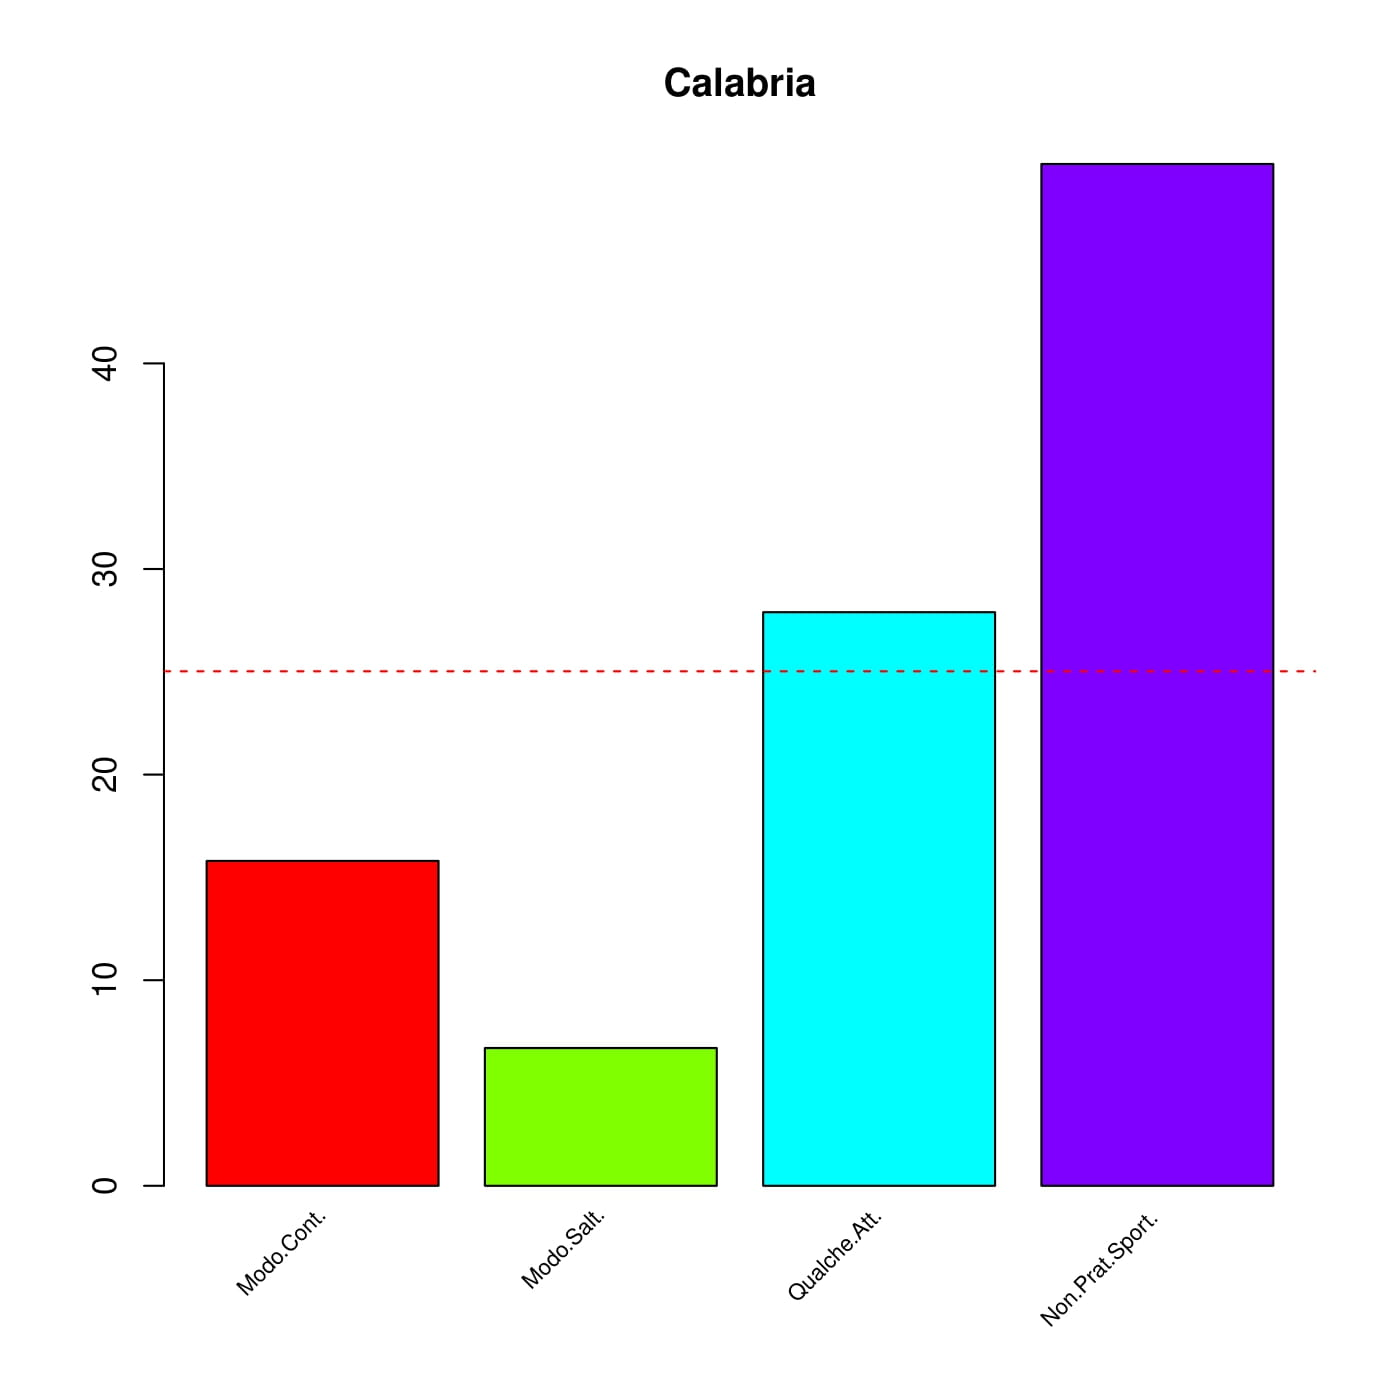
\includegraphics[height=8cm]{ProgettoSAD/capitoli/images/barre_regioni/barre_calabria.jpg}}
        \qquad
\end{figure}

\begin{figure}[!htbp]
    \centering
        \subfloat{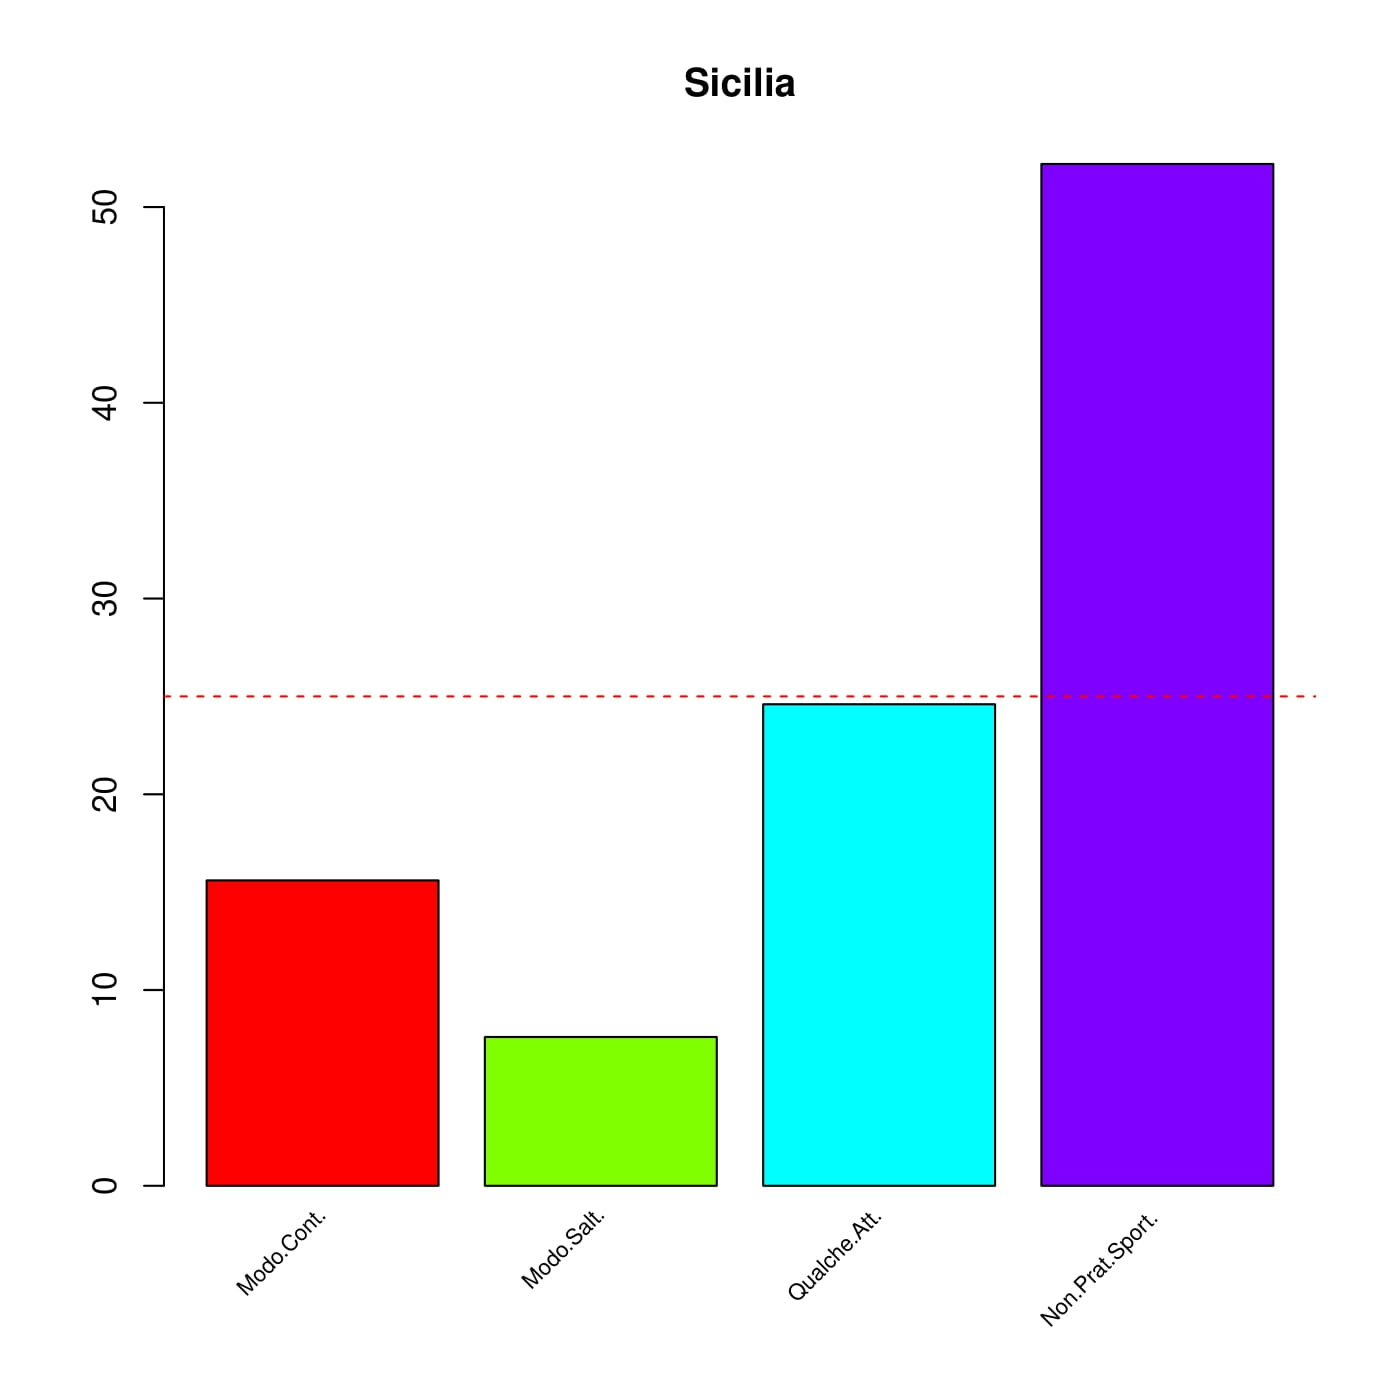
\includegraphics[height=8cm]{ProgettoSAD/capitoli/images/barre_regioni/barre_sicilia.jpg}}
        \qquad
        \subfloat{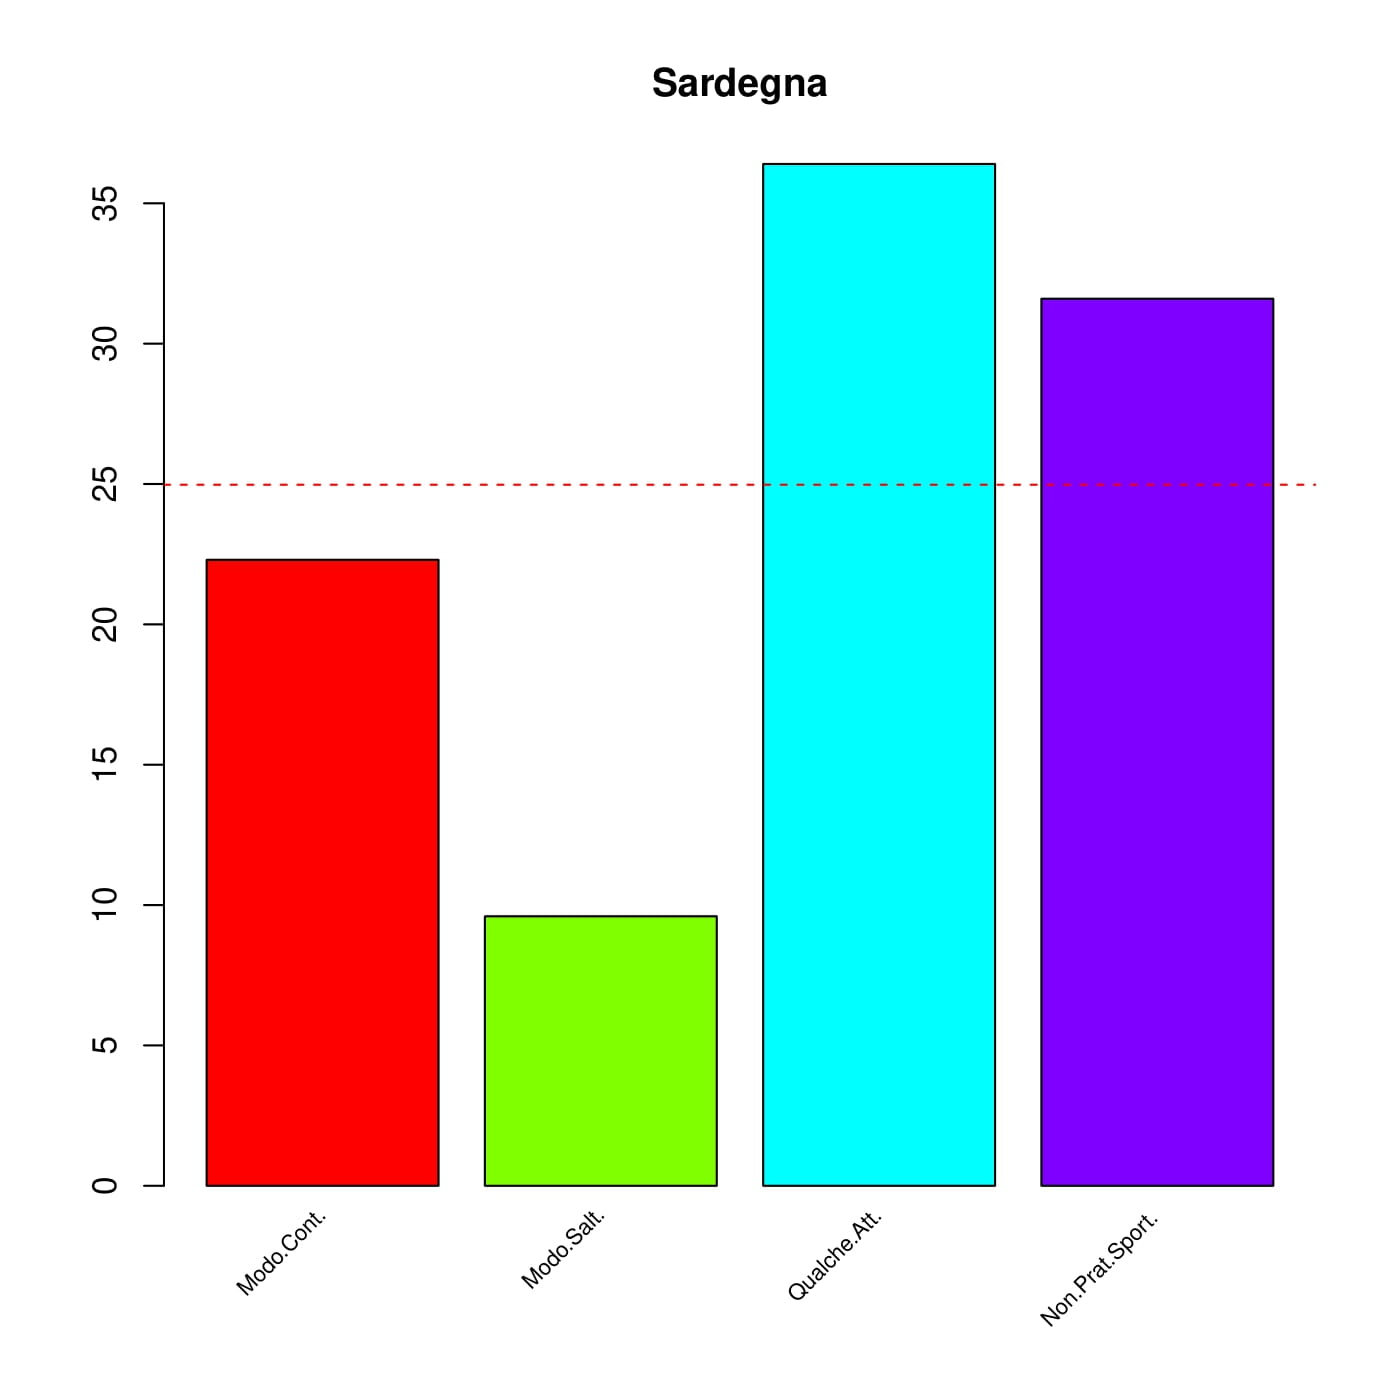
\includegraphics[height=8cm]{ProgettoSAD/capitoli/images/barre_regioni/barre_sardegna.jpg}}
        \qquad
\end{figure}

Dai grafici ottenuti, si può notare che nel Nord e nel centro Italia i più frequenti sono quelli a svolgere attività sportiva costante o qualche attività, mentre nel Sud e nelle Isole a prevalere sono quelli che svolgono qualche attività sportiva o non ne svolgono affatto.



\section{Grafici a torta: Regioni}\label{cap2.3}

In questa sezione verrà mostrato un grafico a torta per ogni regione del dataset, al fine di poter analizzare la densità di pratica sportiva in relazione alla totalità.

\noindent \textbf{Costruzione Grafico a torta}

È possibile impiegare nuovamente la funzione \textit{estraiRiga()} per creare i grafici a torta per le regioni.

\vspace{5mm}
\begin{lstlisting}
 index <- 1
  for (element in regioni) {
    pie1 <- pie(estraiRiga(df, index),
                labels = names(df),
                main = element,
                col = rainbow(5))
    index <- index + 1
  }
\end{lstlisting}
\vspace{5mm}

\begin{figure}[!htbp]
    \centering
        \subfloat{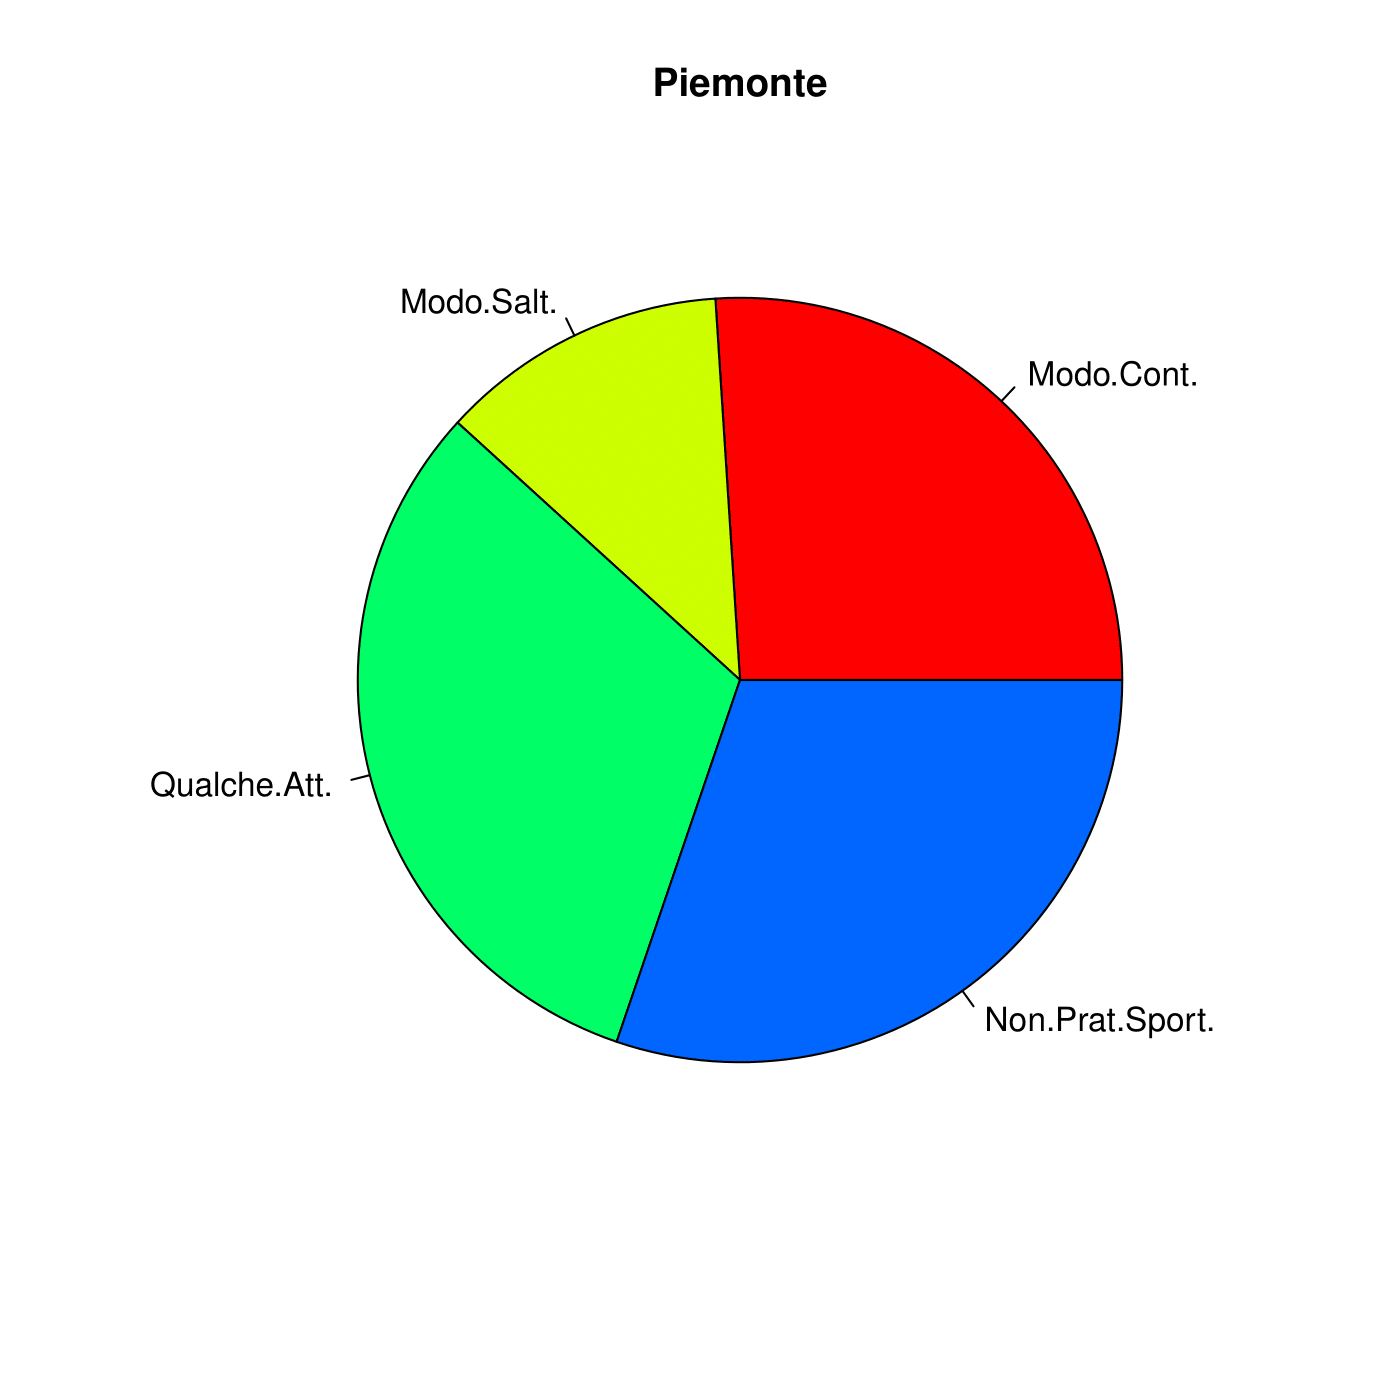
\includegraphics[height=8cm]{ProgettoSAD/capitoli/images/torta_regioni/torta_piemonte.png}}
        \qquad
        \subfloat{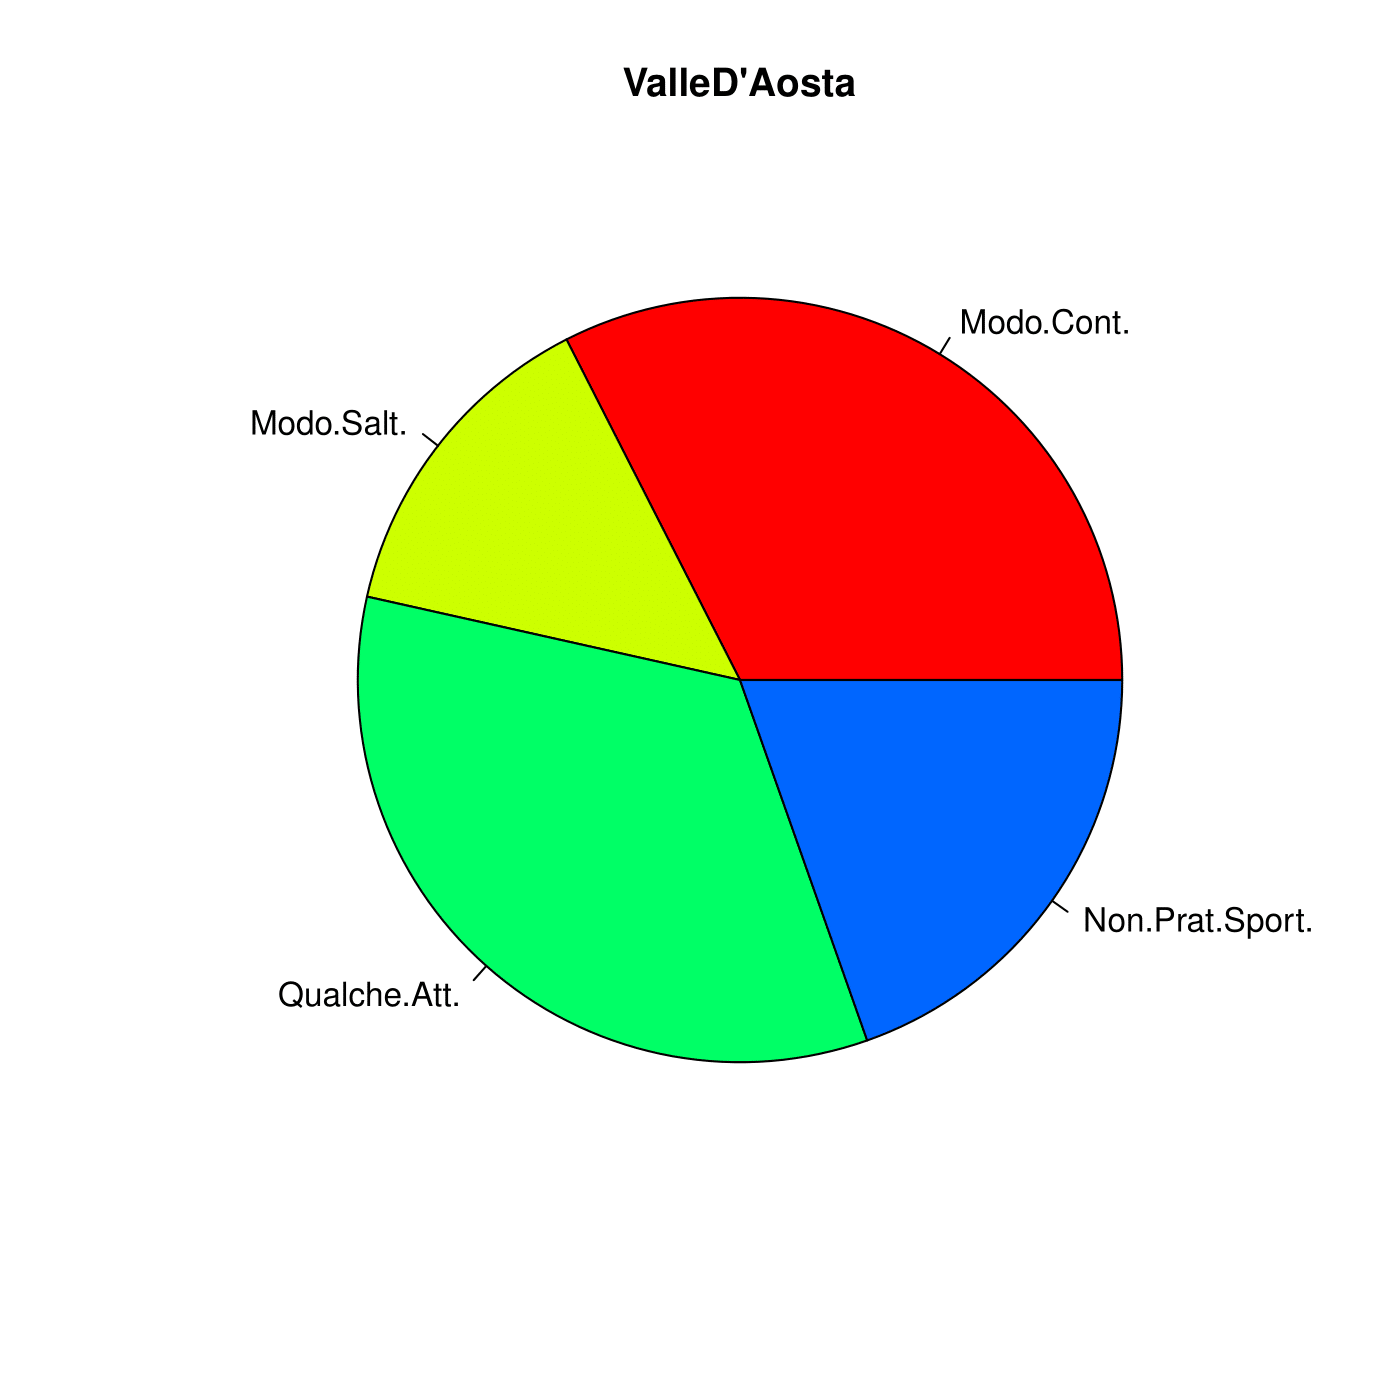
\includegraphics[height=8cm]{ProgettoSAD/capitoli/images/torta_regioni/torta_valledaosta.png}}
        \qquad
\end{figure}

\begin{figure}[!htbp]
    \centering
        \subfloat{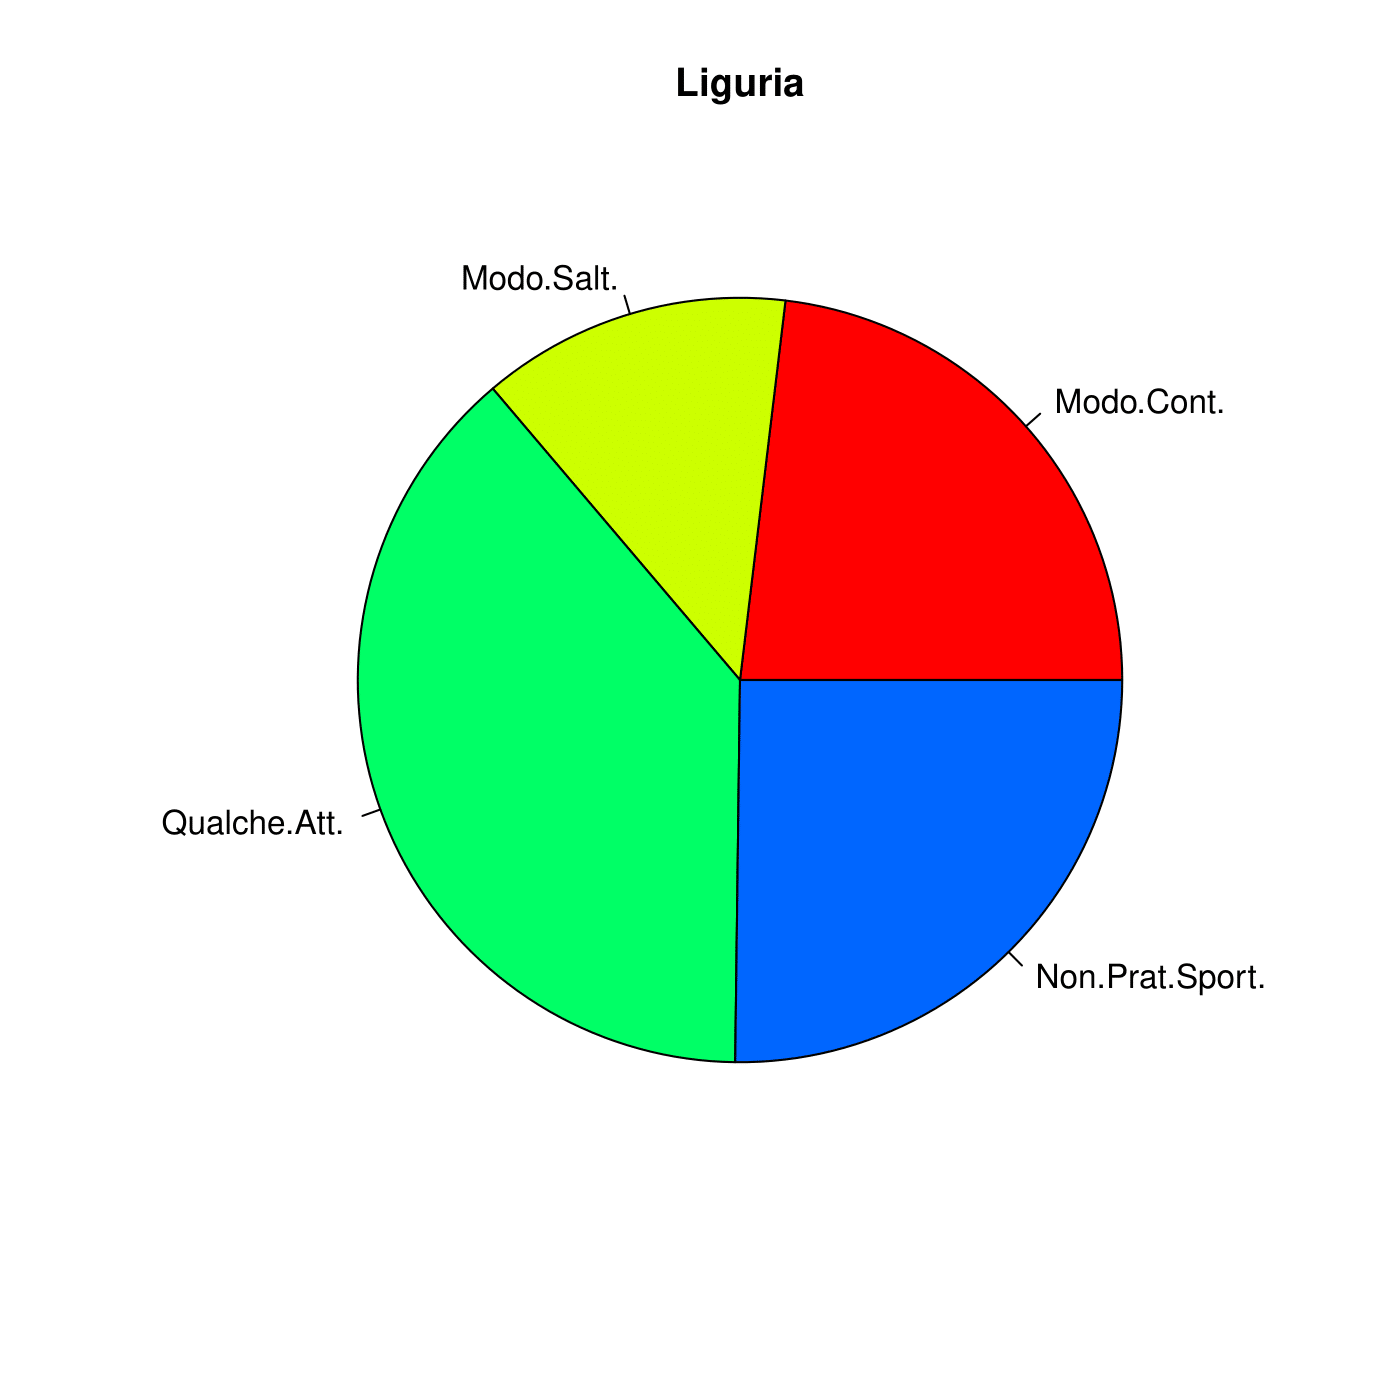
\includegraphics[height=8cm]{ProgettoSAD/capitoli/images/torta_regioni/torta_liguria.png}}
        \qquad
        \subfloat{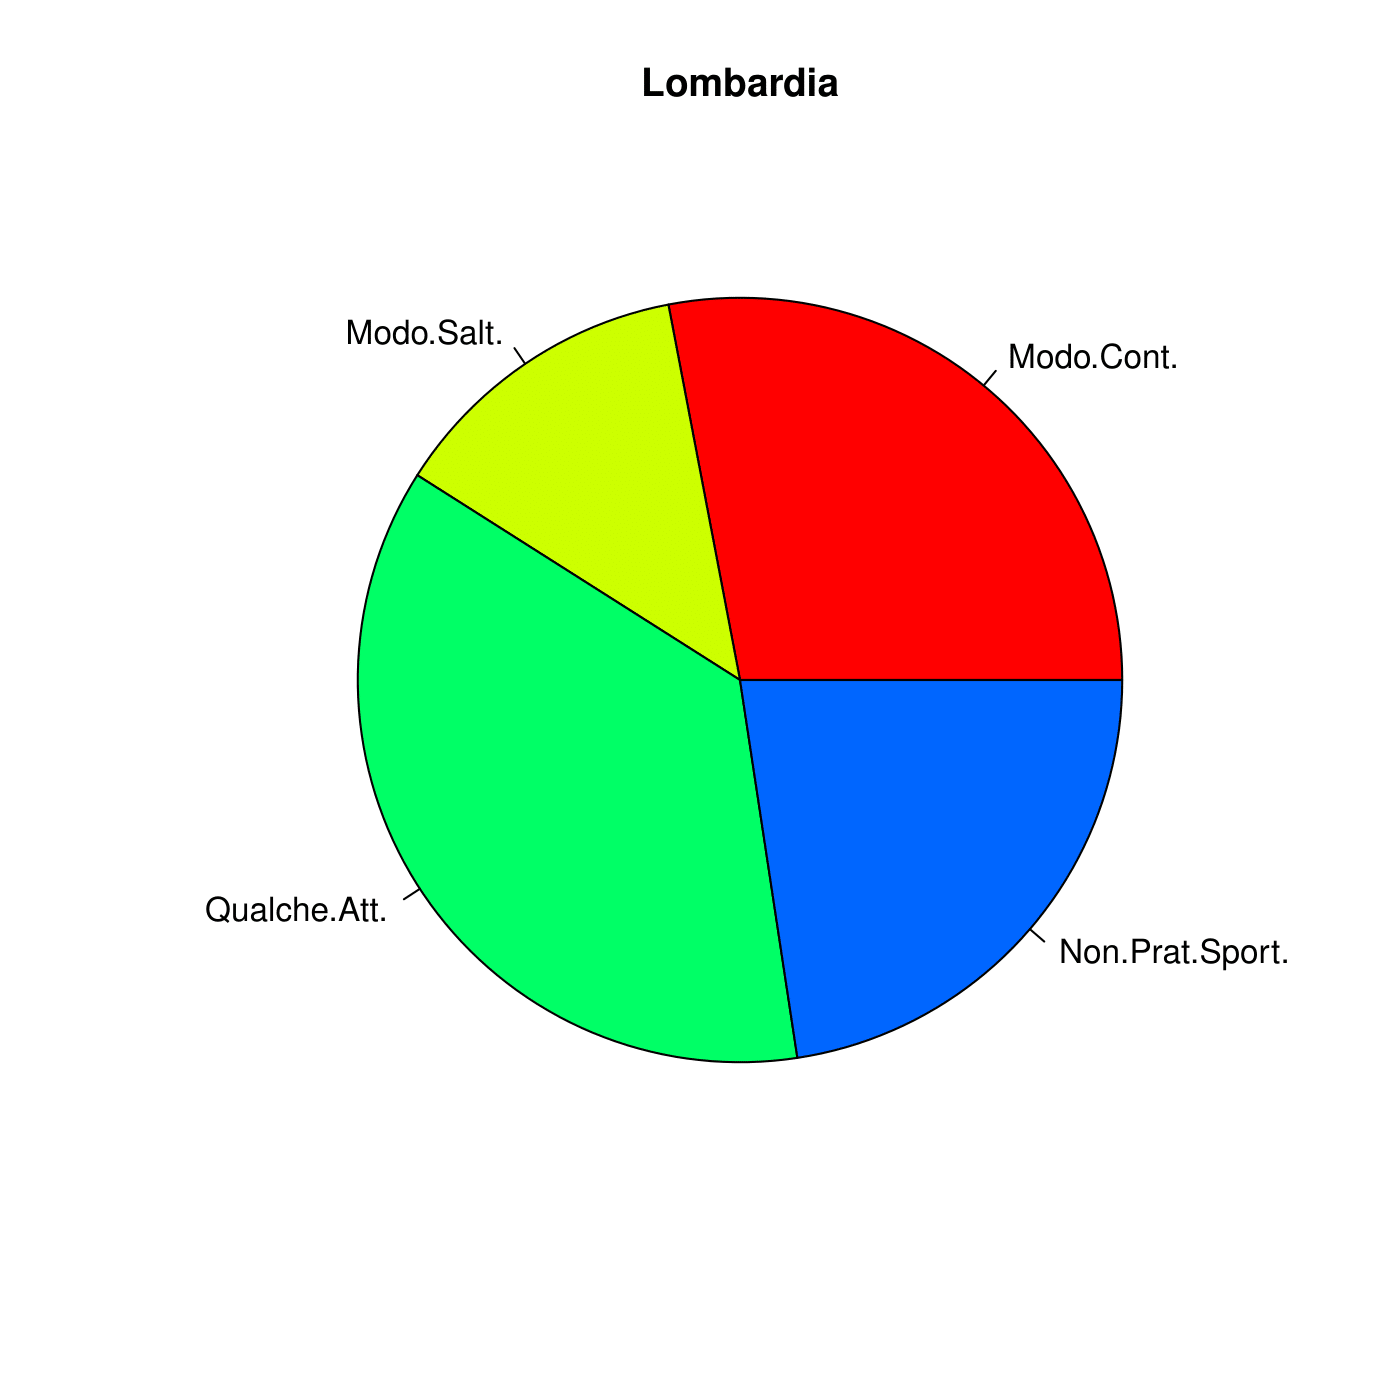
\includegraphics[height=8cm]{ProgettoSAD/capitoli/images/torta_regioni/torta_lombardia.png}}
        \qquad
\end{figure}
\begin{figure}[!htbp]
    \centering
        \subfloat{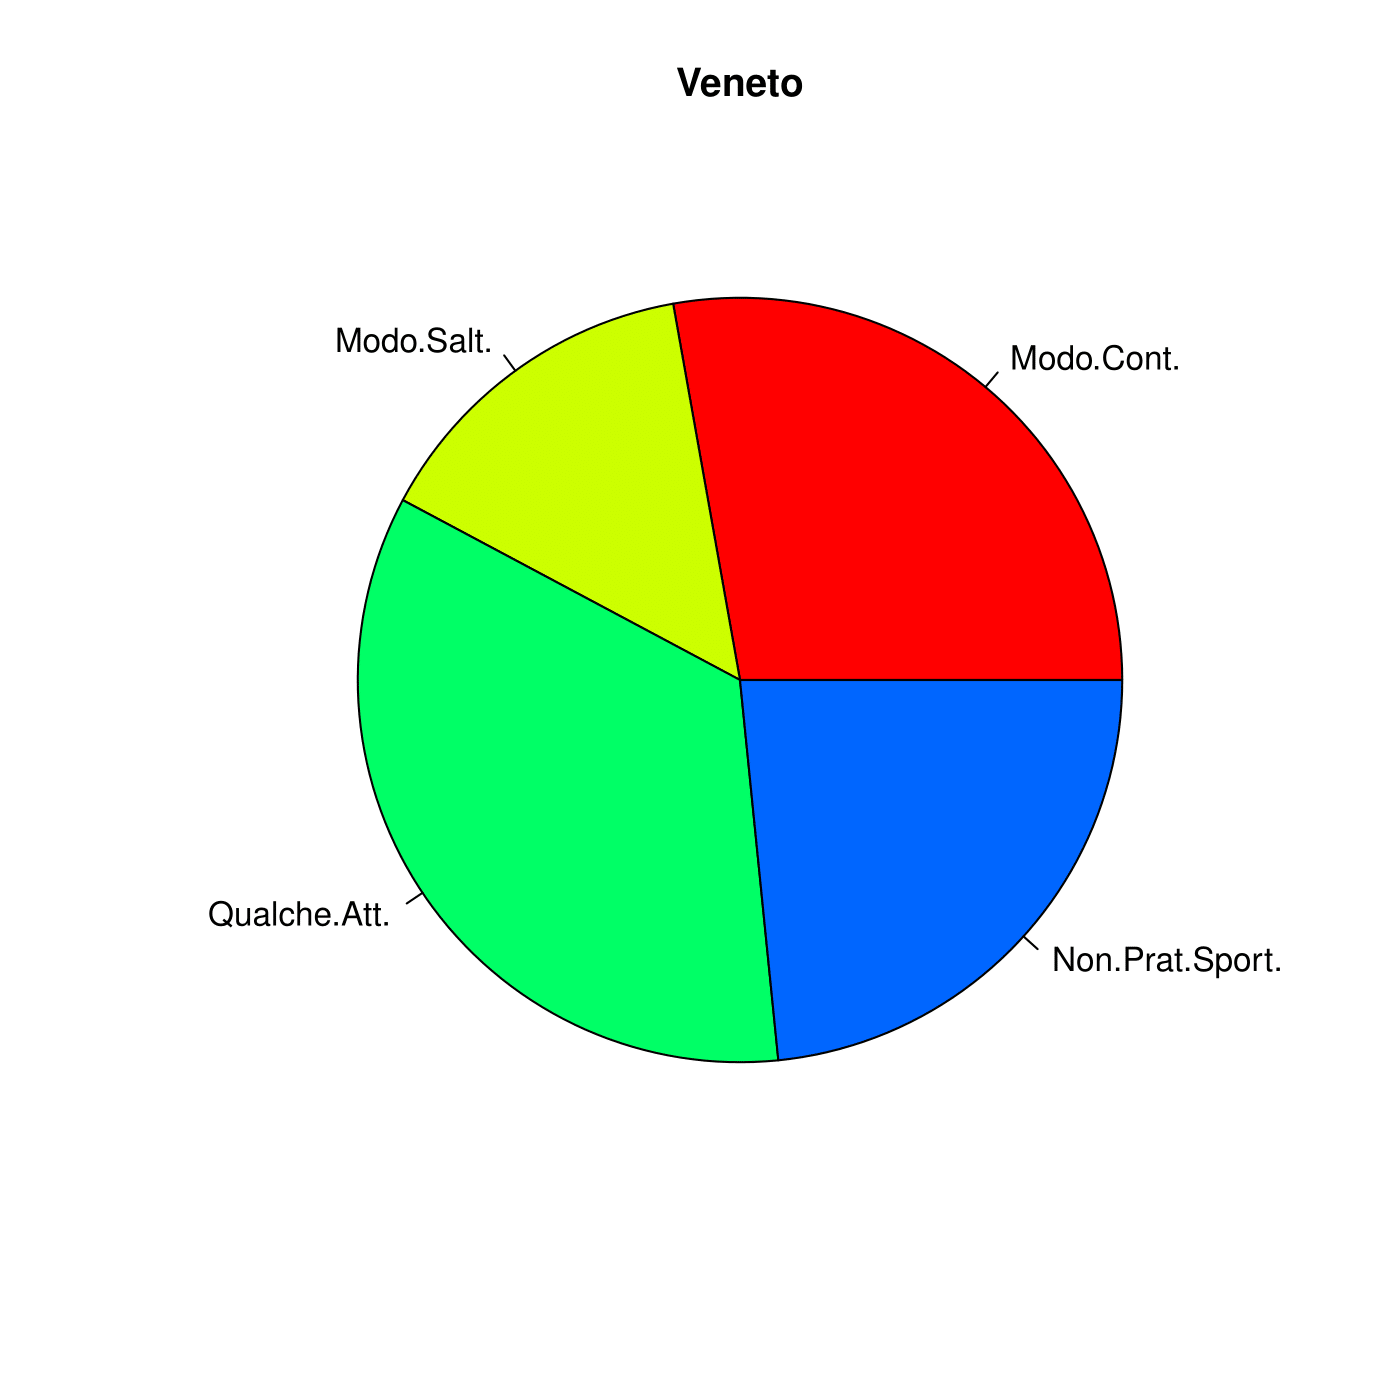
\includegraphics[height=8cm]{ProgettoSAD/capitoli/images/torta_regioni/torta_veneto.png}}
        \qquad
        \subfloat{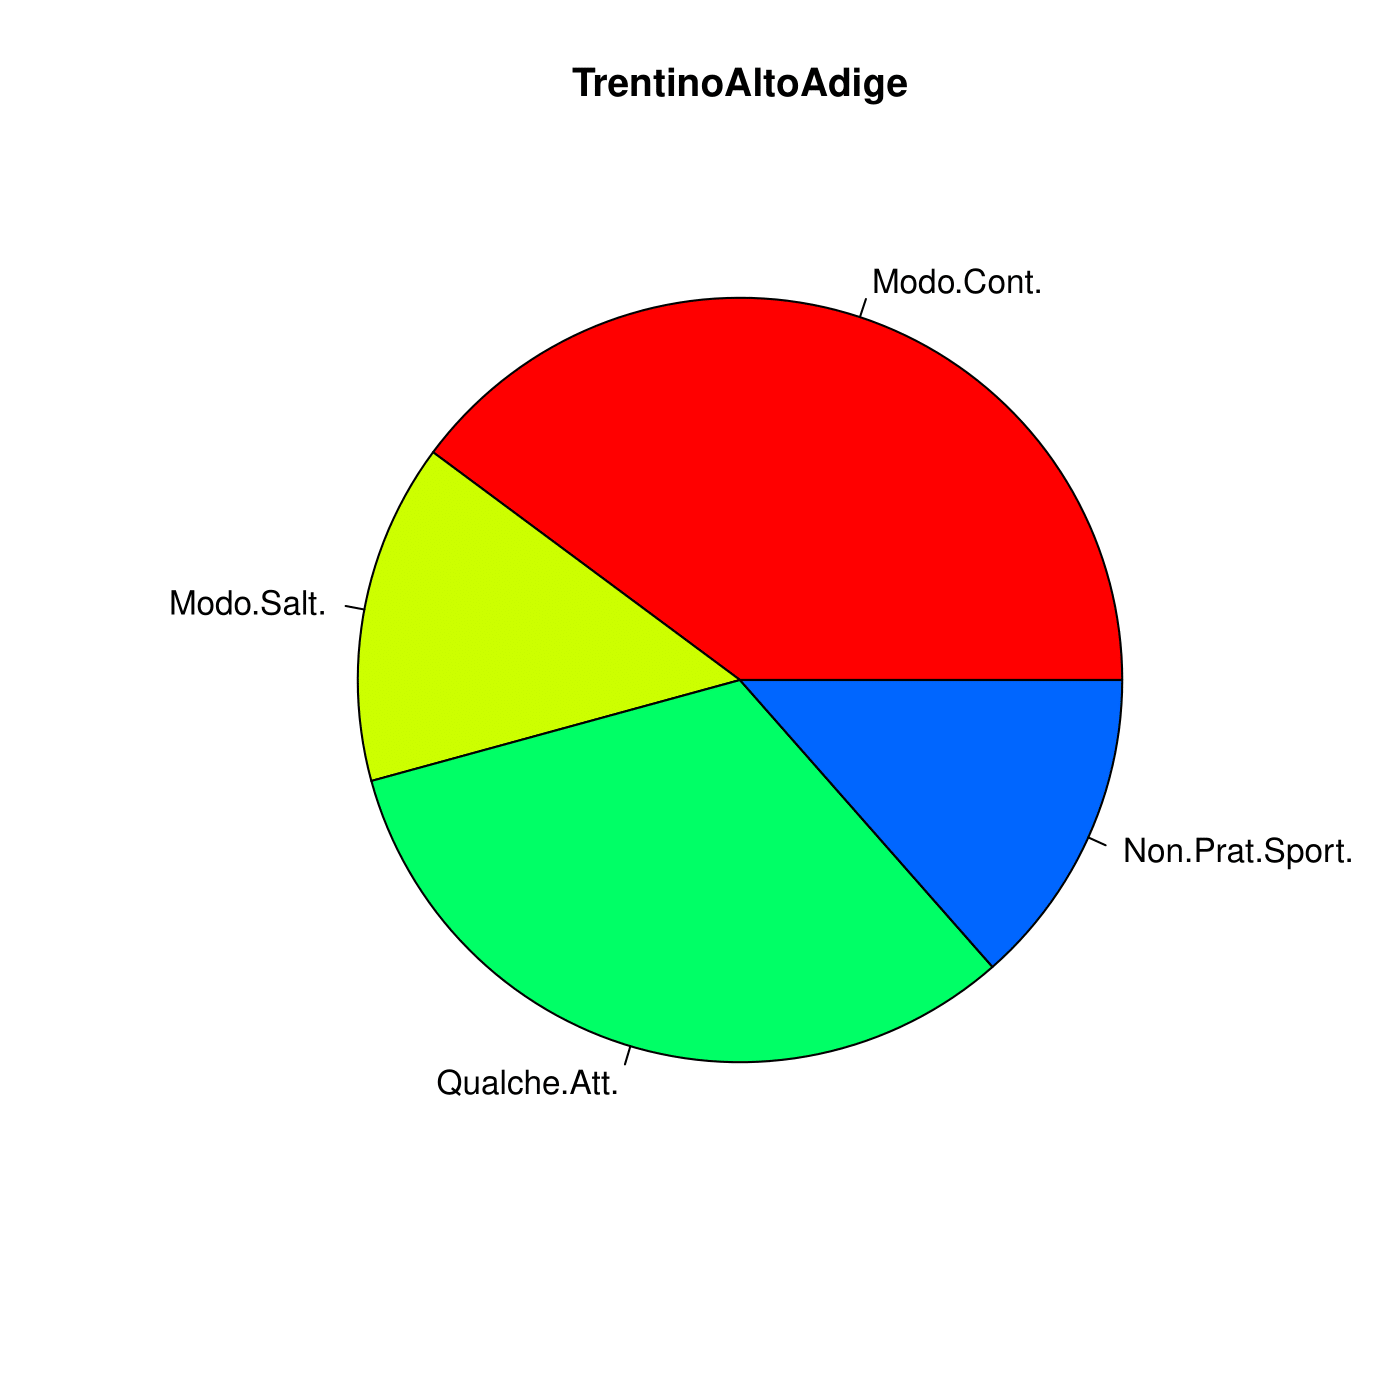
\includegraphics[height=8cm]{ProgettoSAD/capitoli/images/torta_regioni/trentino.png}}
        \qquad
\end{figure}
\begin{figure}[!htbp]
    \centering
        \subfloat{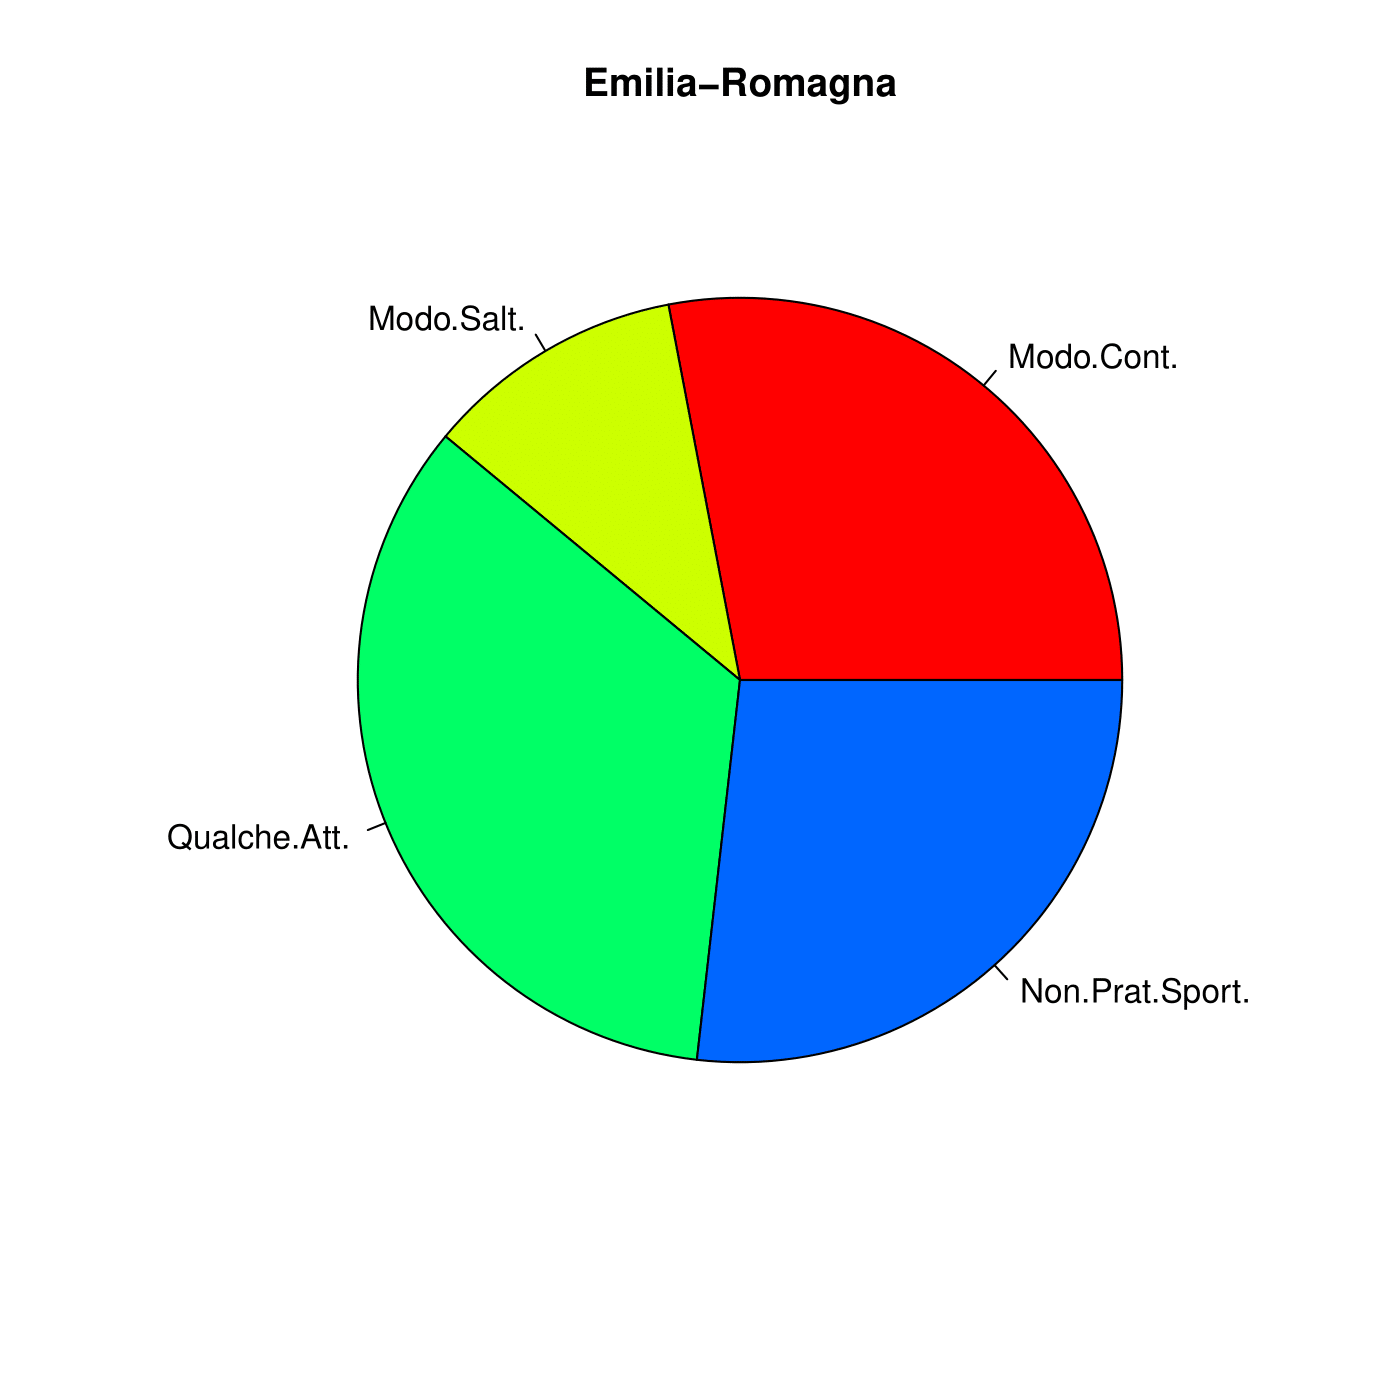
\includegraphics[height=8cm]{ProgettoSAD/capitoli/images/torta_regioni/torta_emilia.png}}
        \qquad
        \subfloat{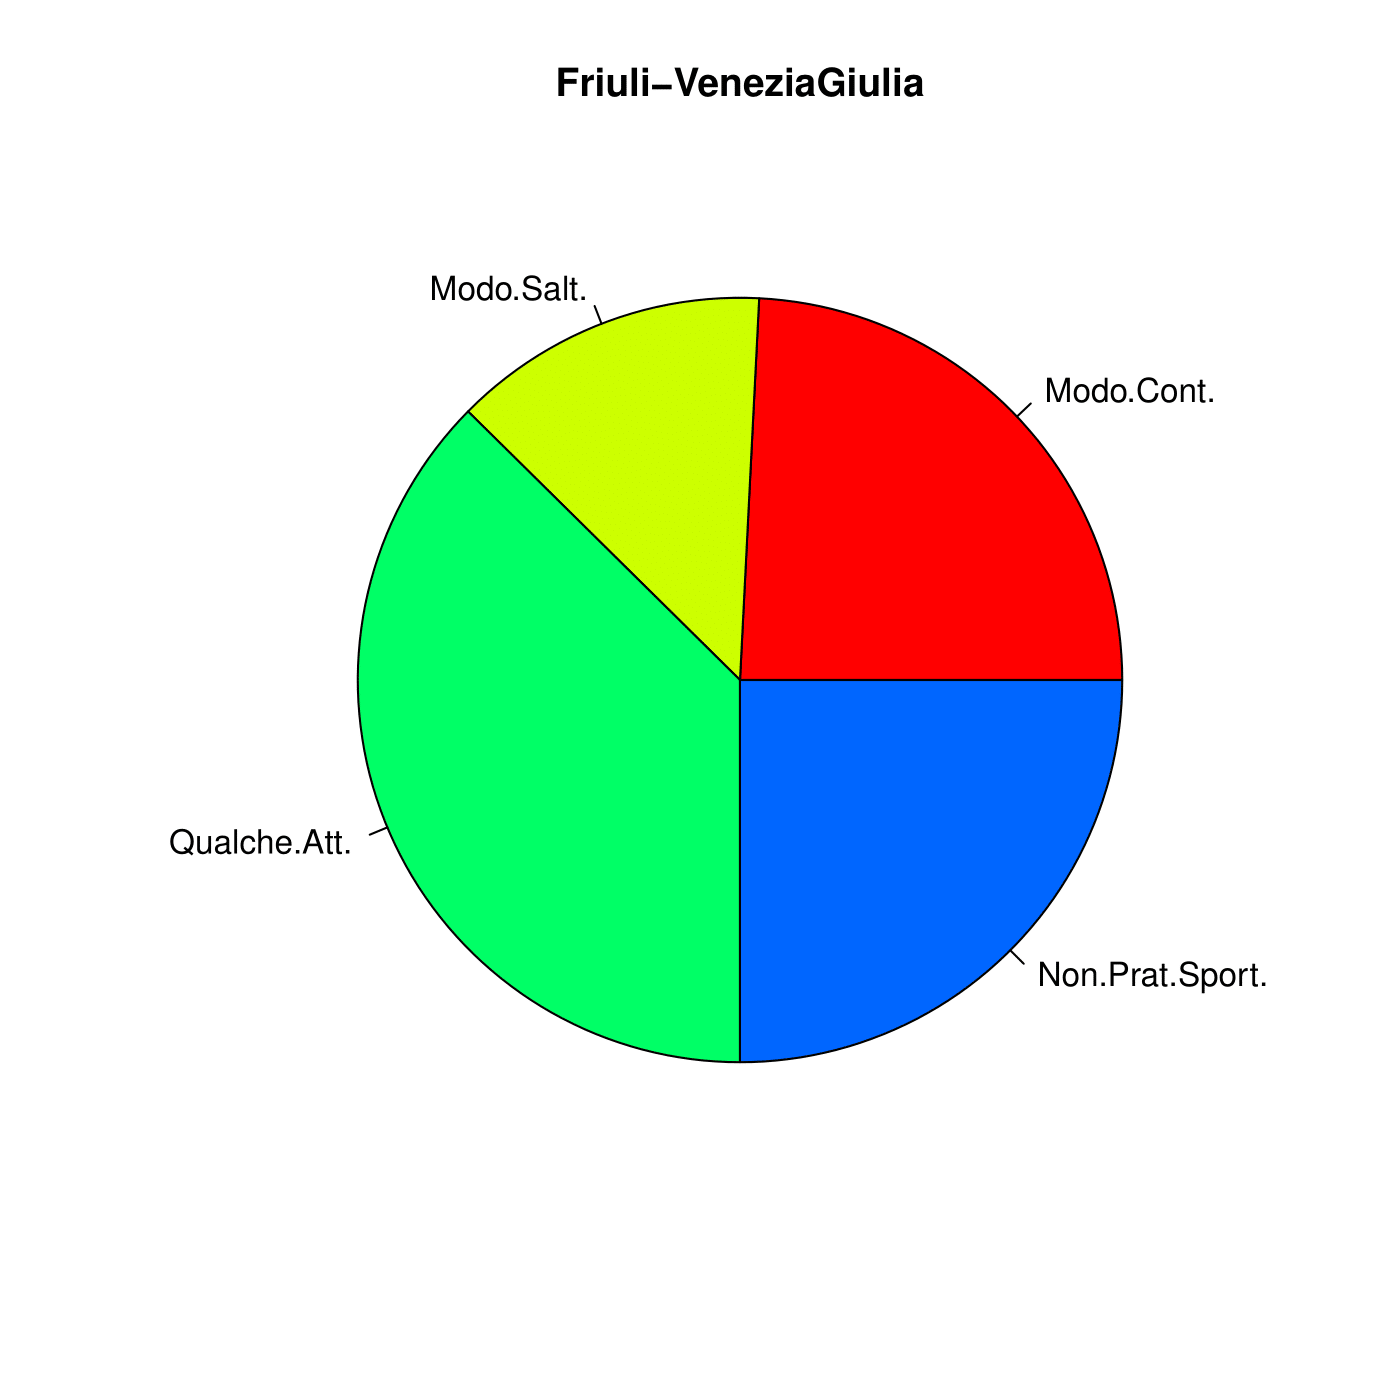
\includegraphics[height=8cm]{ProgettoSAD/capitoli/images/torta_regioni/torta_friuli.png}}
        \qquad
\end{figure}
\begin{figure}[!htbp]
    \centering
        \subfloat{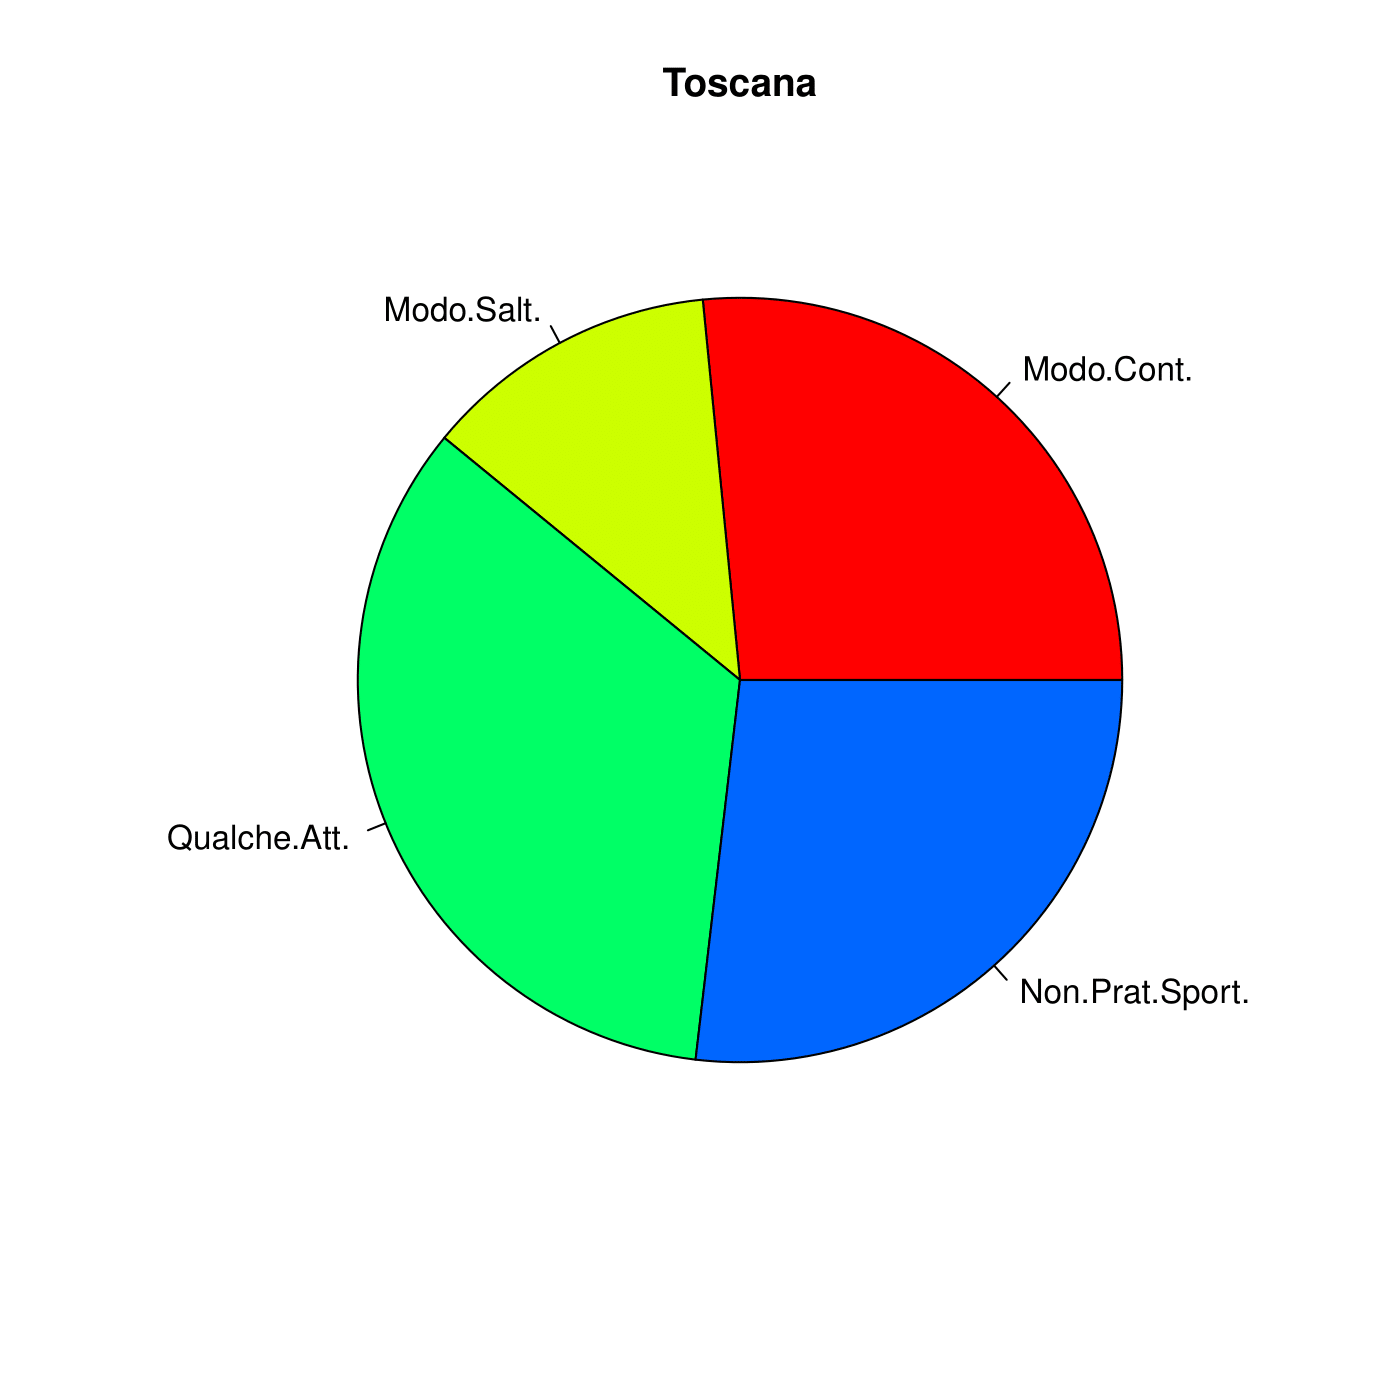
\includegraphics[height=8cm]{ProgettoSAD/capitoli/images/torta_regioni/torta_toscana.png}}
        \qquad
        \subfloat{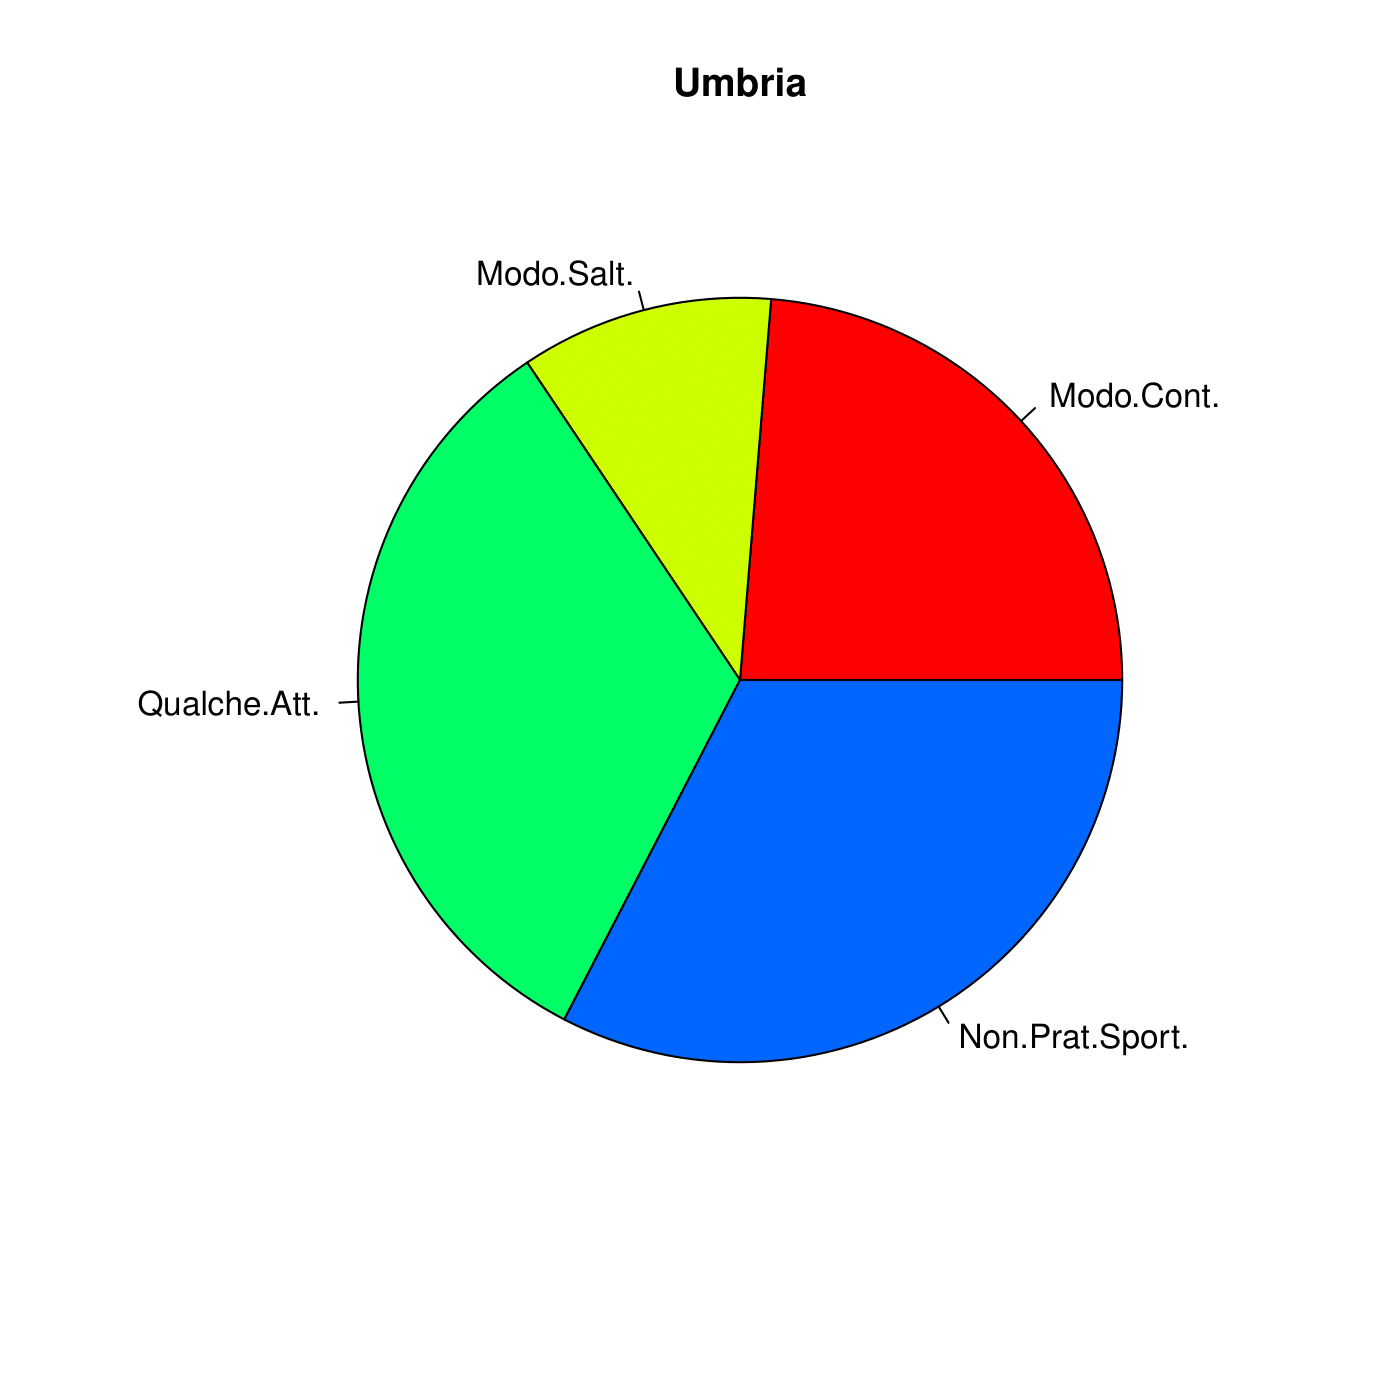
\includegraphics[height=8cm]{ProgettoSAD/capitoli/images/torta_regioni/torta_umbria.png}}
        \qquad
\end{figure}
\begin{figure}[!htbp]
    \centering
        \subfloat{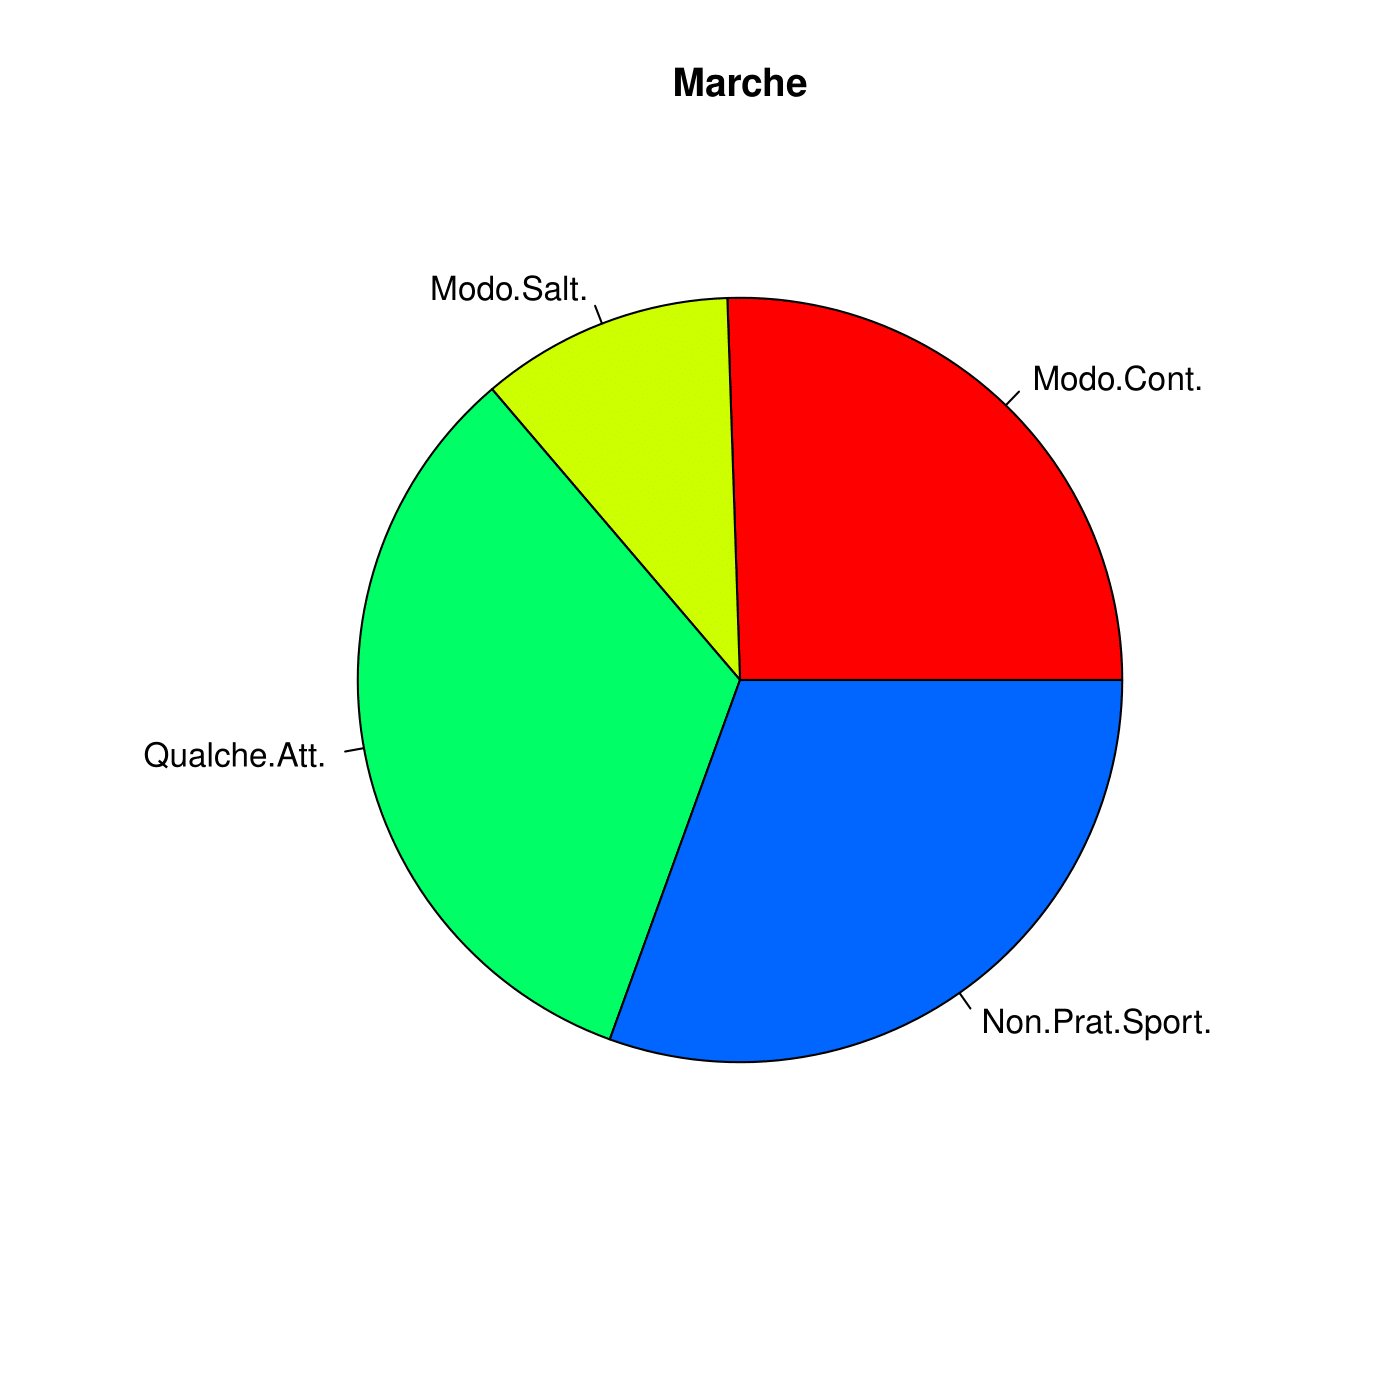
\includegraphics[height=8cm]{ProgettoSAD/capitoli/images/torta_regioni/torta_marche.png}}
        \qquad
        \subfloat{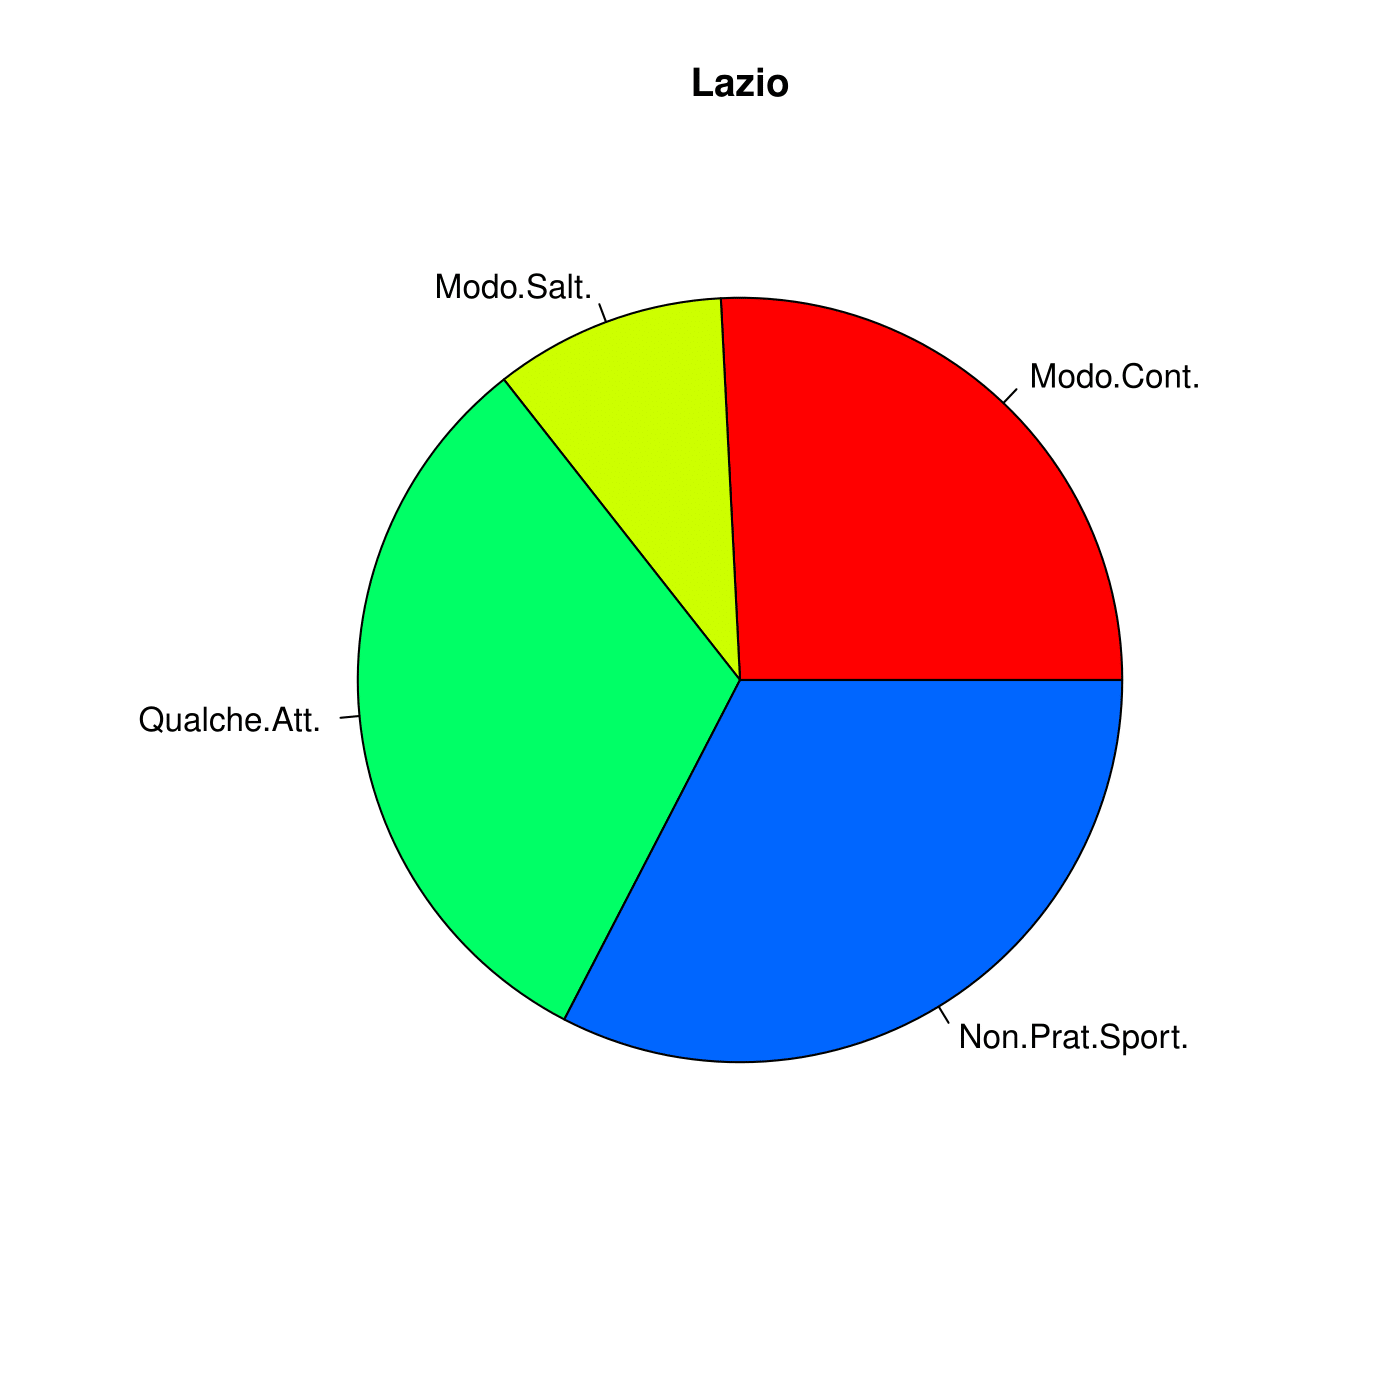
\includegraphics[height=8cm]{ProgettoSAD/capitoli/images/torta_regioni/torta_lazio.png}}
        \qquad
\end{figure}
\begin{figure}[!htbp]
    \centering
        \subfloat{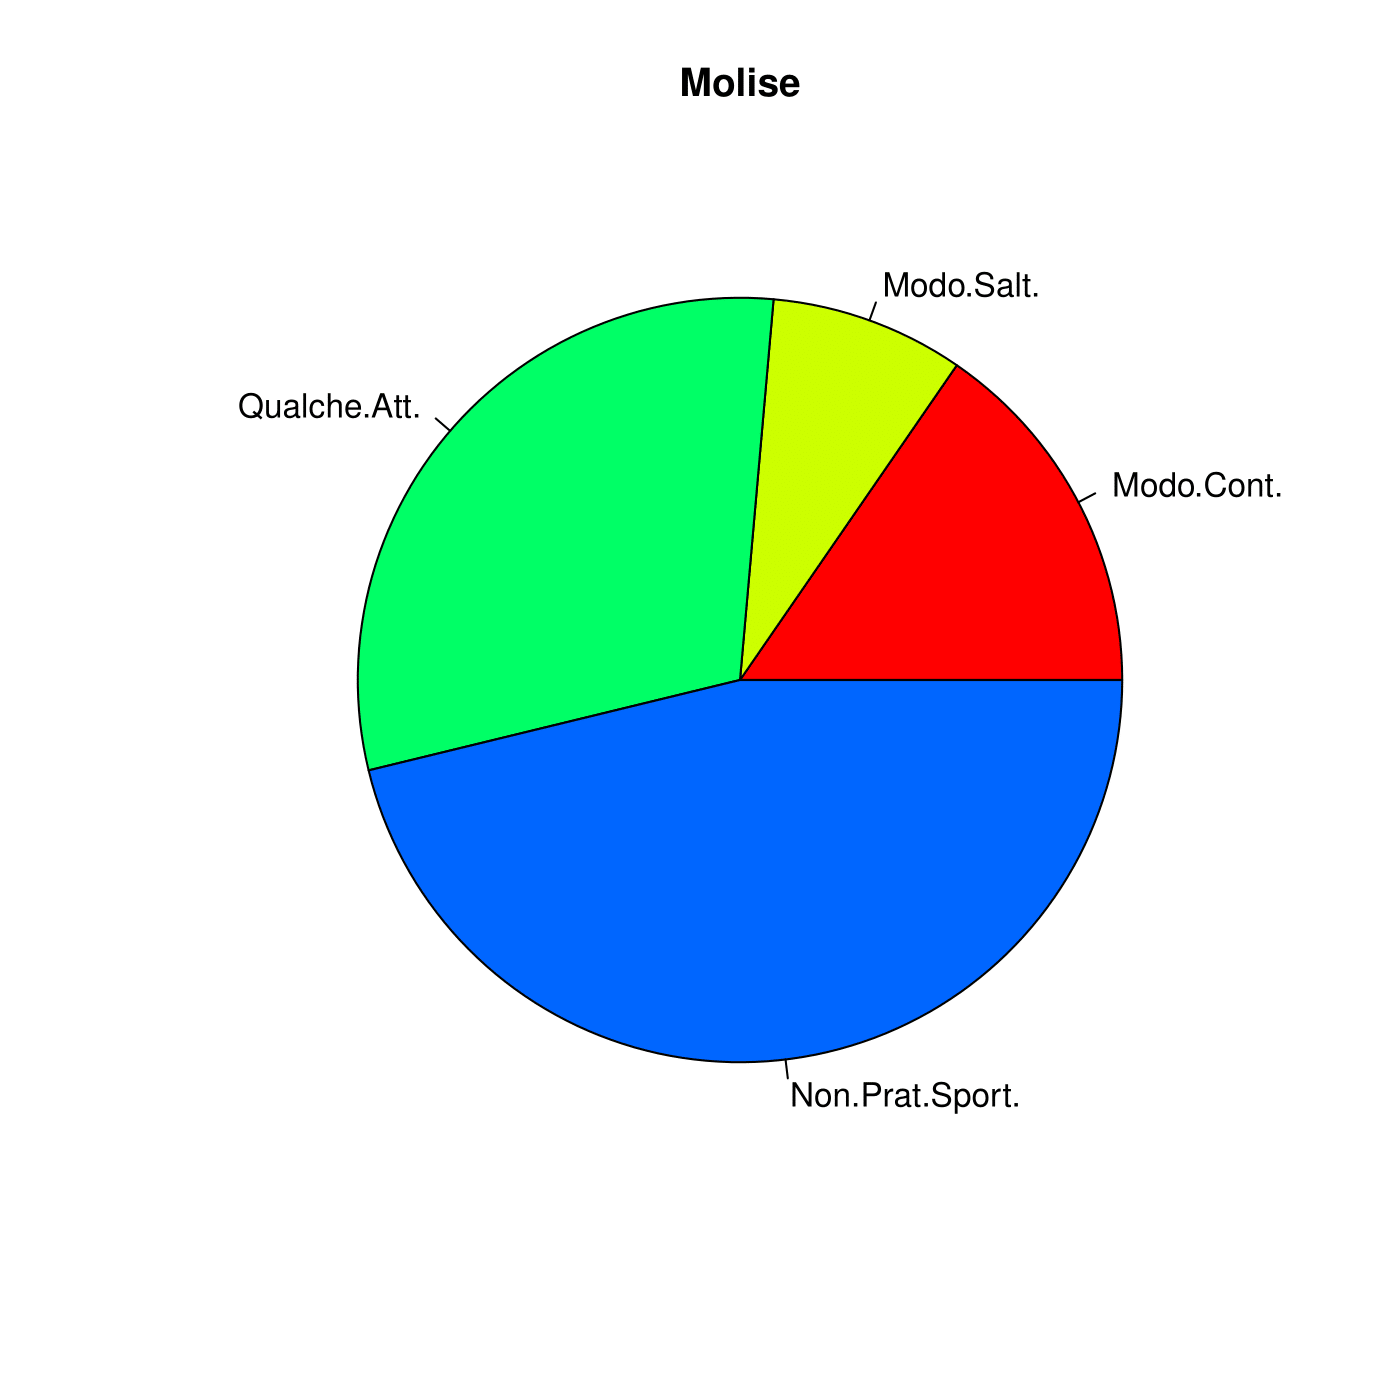
\includegraphics[height=8cm]{ProgettoSAD/capitoli/images/torta_regioni/torta_molise.png}}
        \qquad
        \subfloat{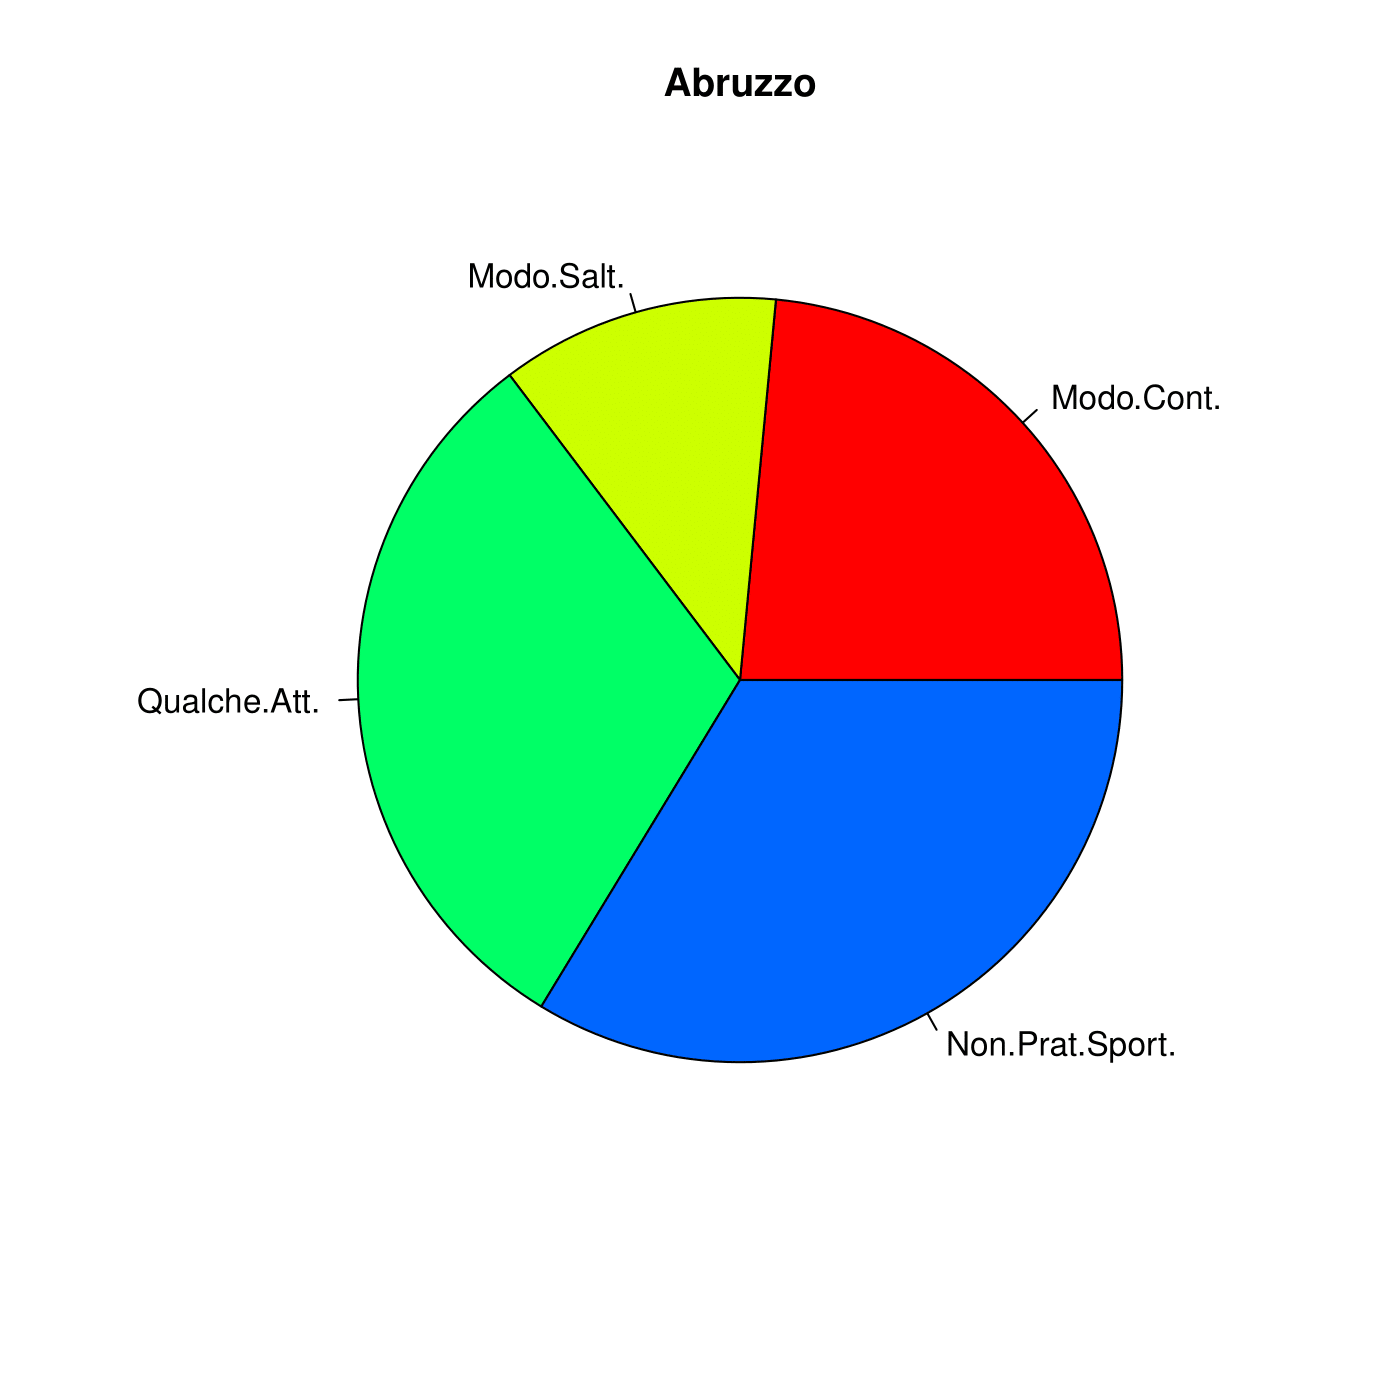
\includegraphics[height=8cm]{ProgettoSAD/capitoli/images/torta_regioni/torta_abruzzo.png}}
        \qquad
\end{figure}
\begin{figure}[!htbp]
    \centering
        \subfloat{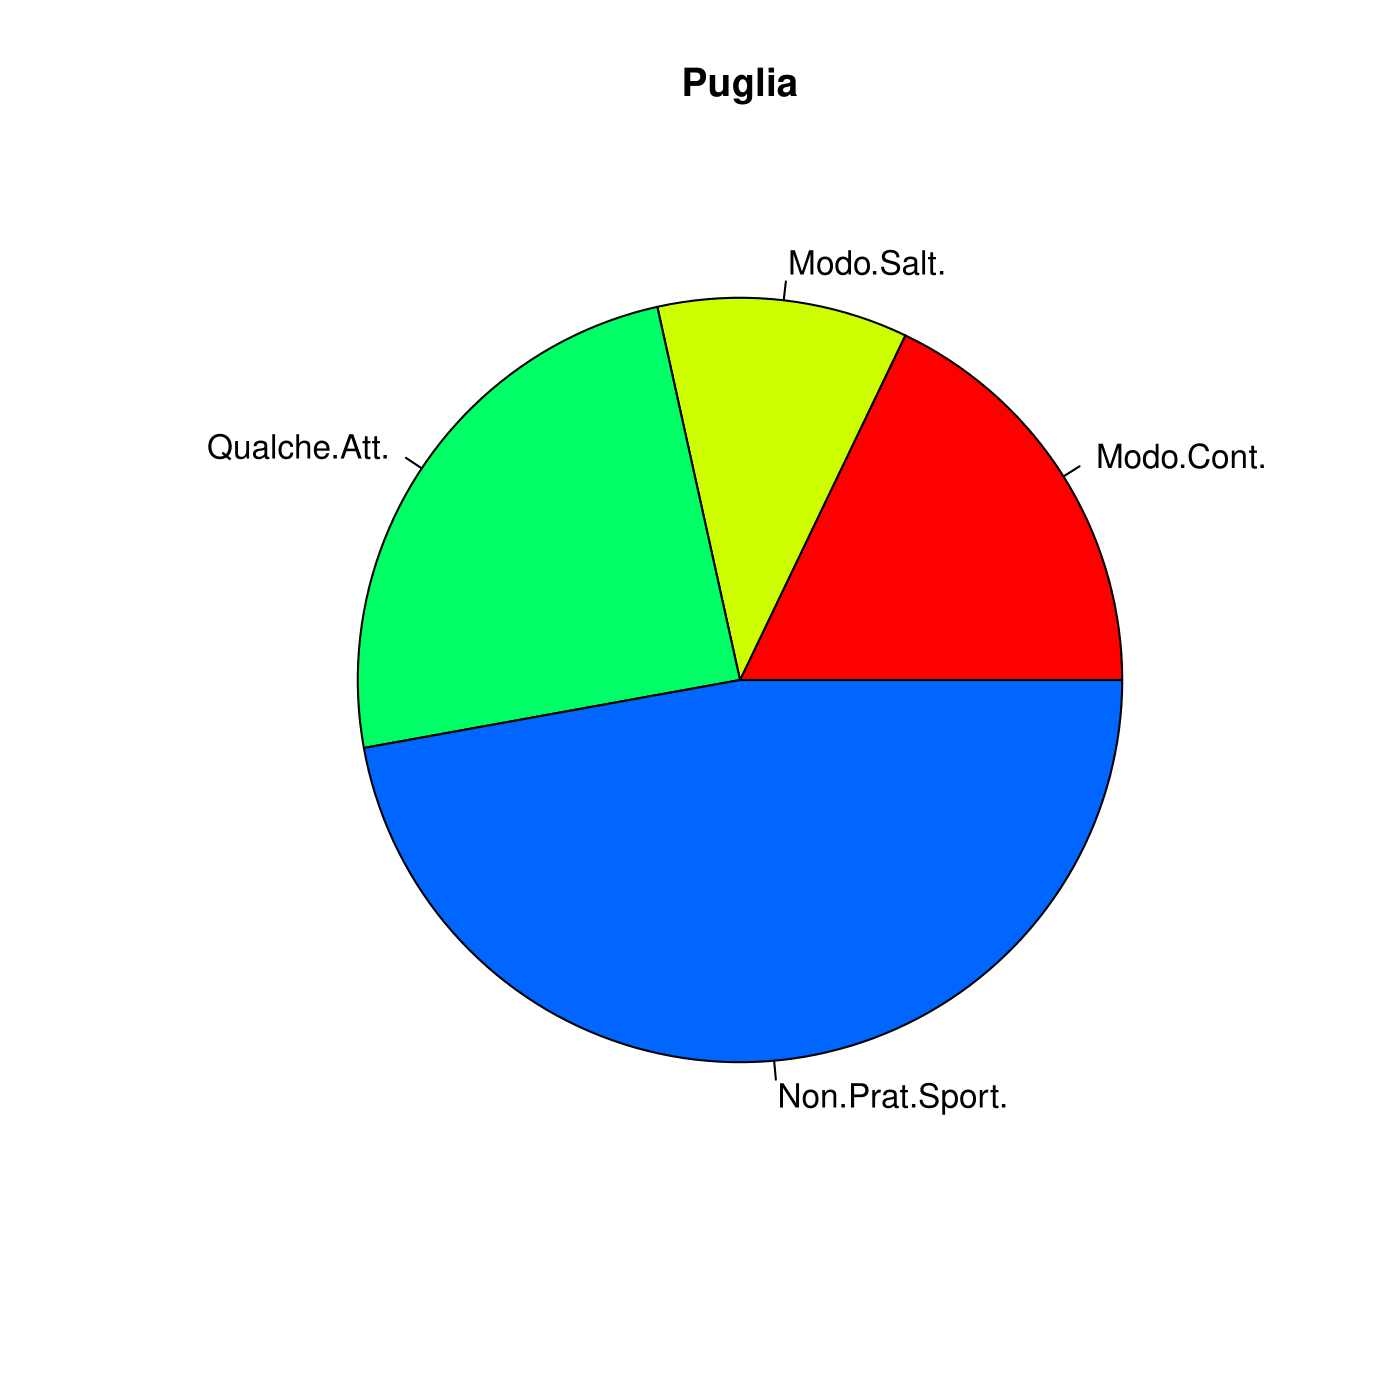
\includegraphics[height=8cm]{ProgettoSAD/capitoli/images/torta_regioni/torta_puglia.png}}
        \qquad
        \subfloat{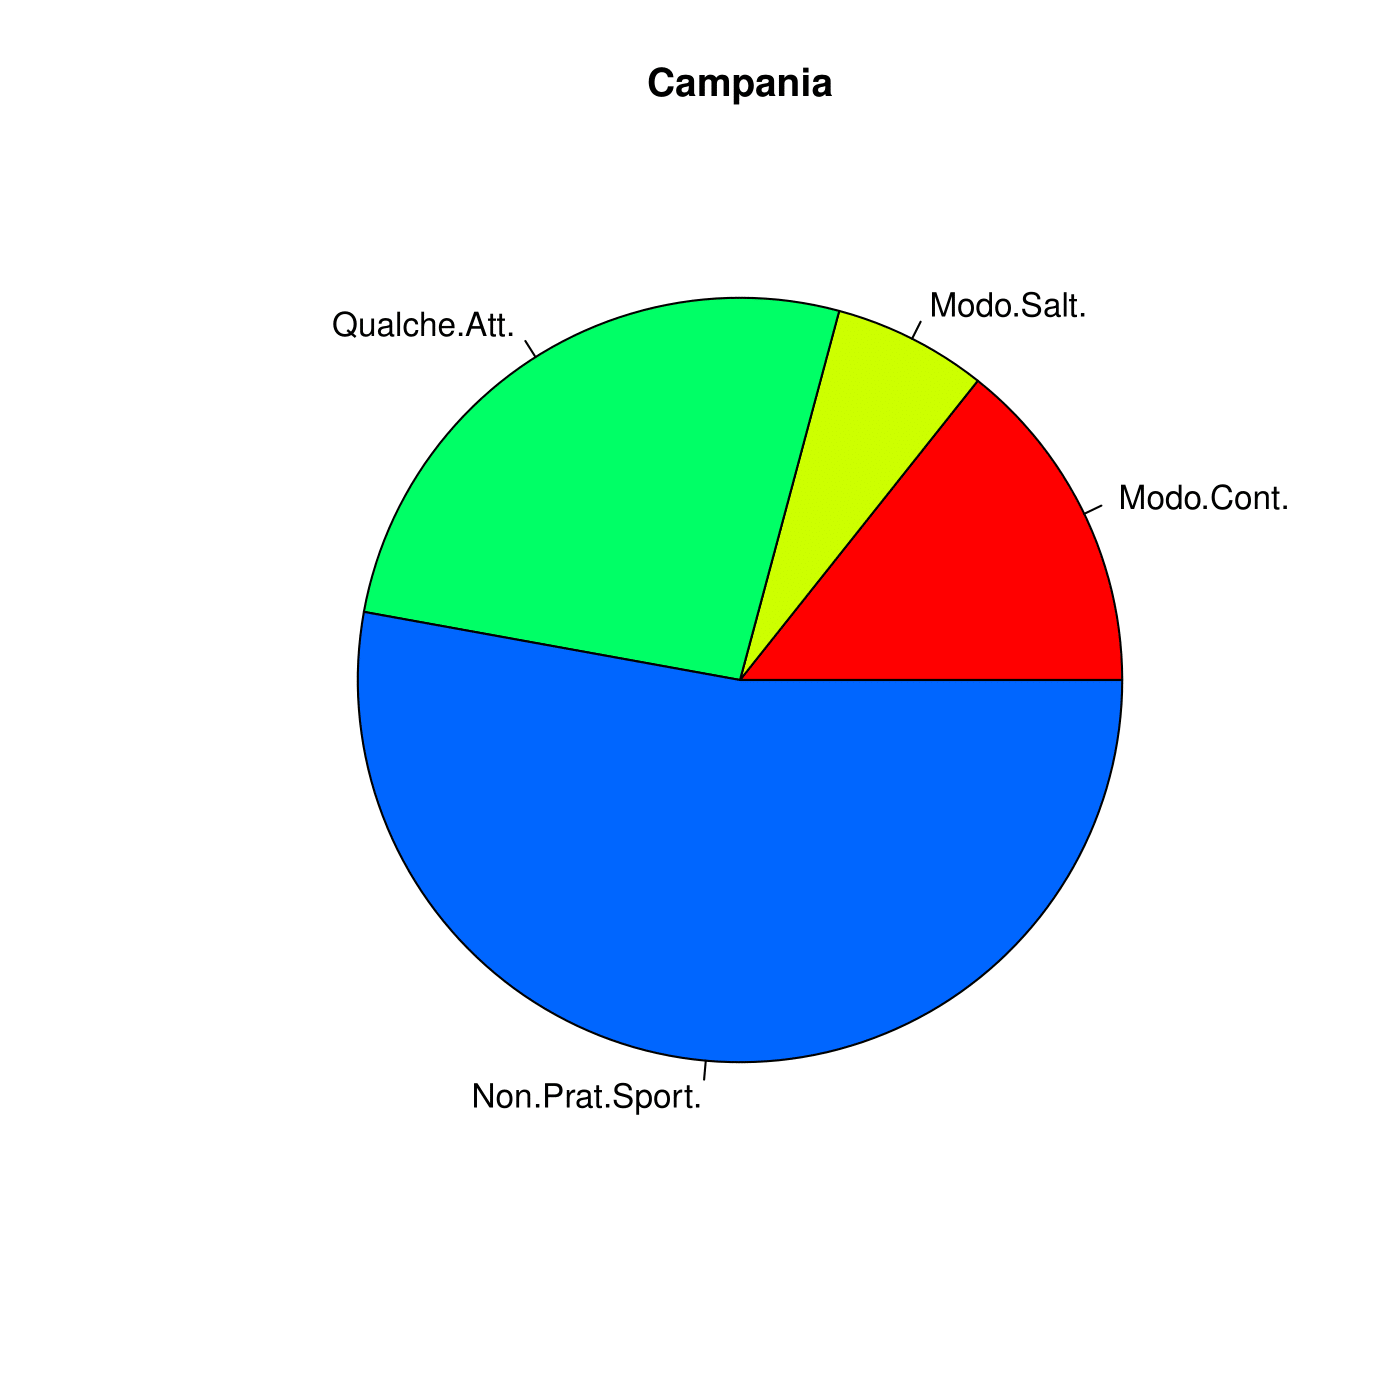
\includegraphics[height=8cm]{ProgettoSAD/capitoli/images/torta_regioni/torta_campania.png}}
        \qquad
\end{figure}
\begin{figure}[!htbp]
    \centering
        \subfloat{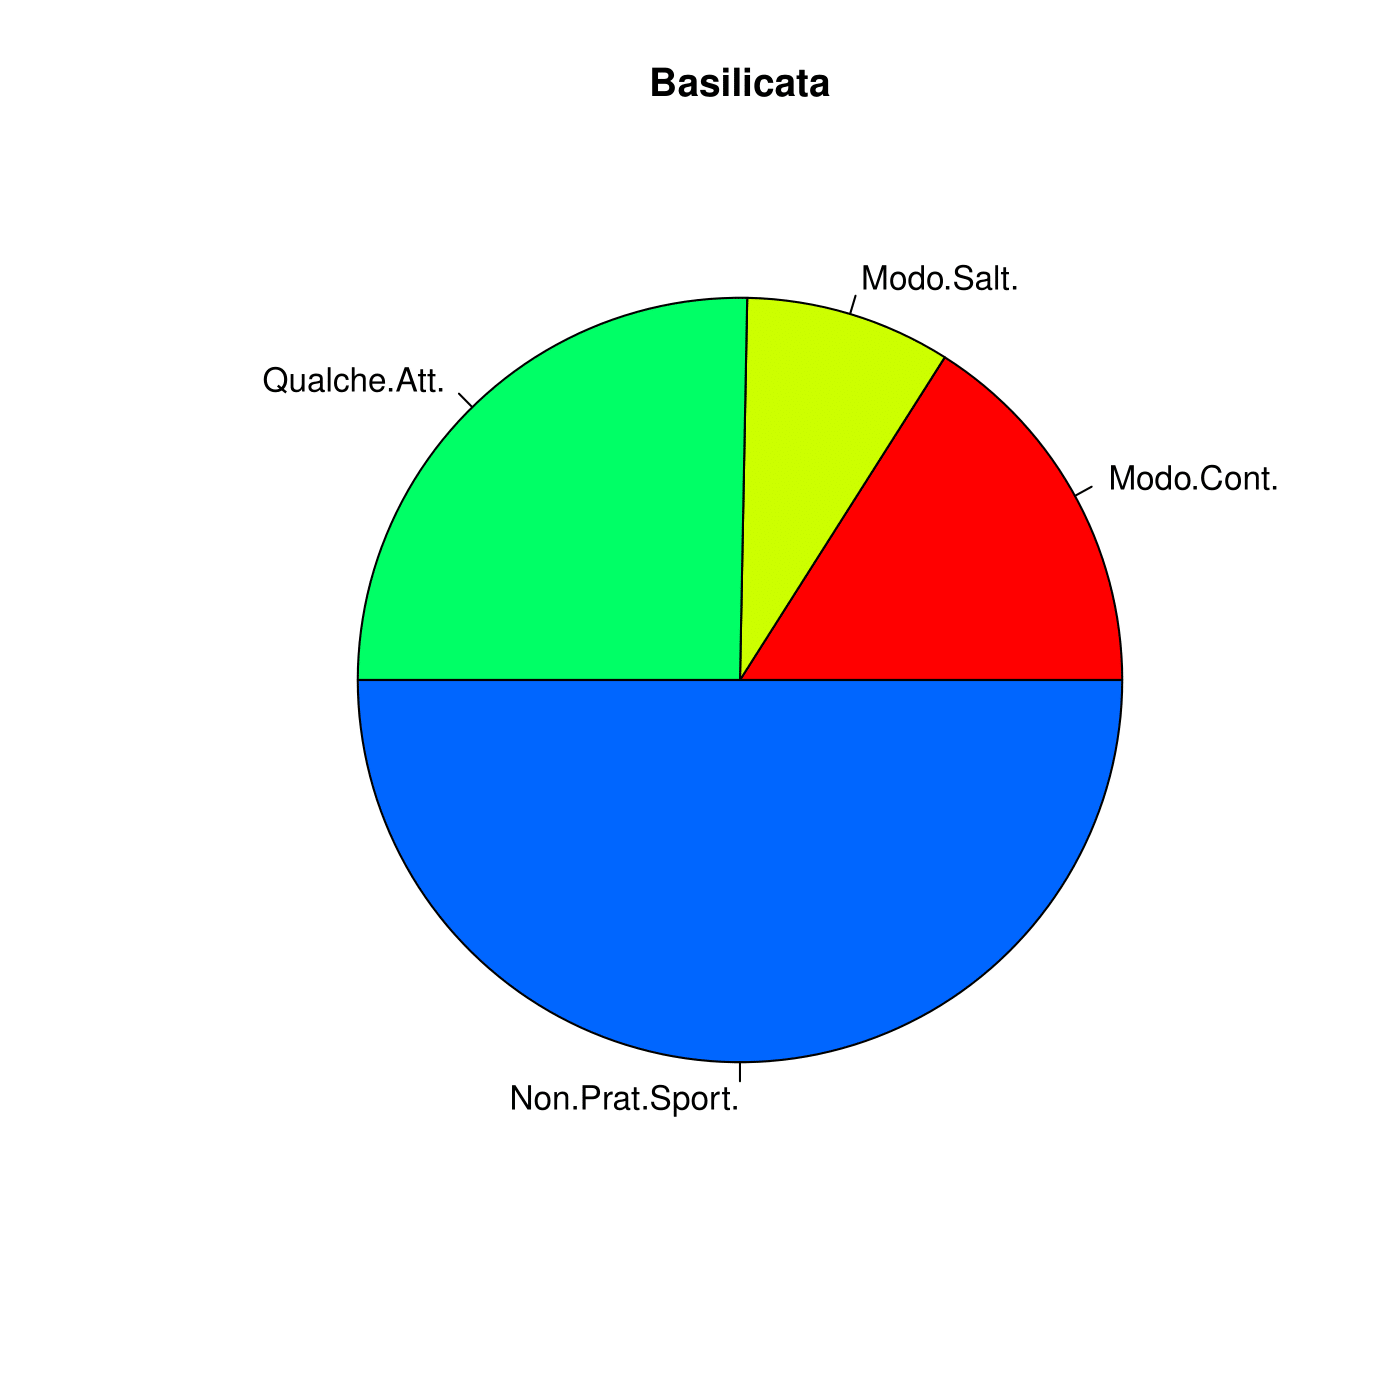
\includegraphics[height=8cm]{ProgettoSAD/capitoli/images/torta_regioni/torta_basilicata.png}}
        \qquad
        \subfloat{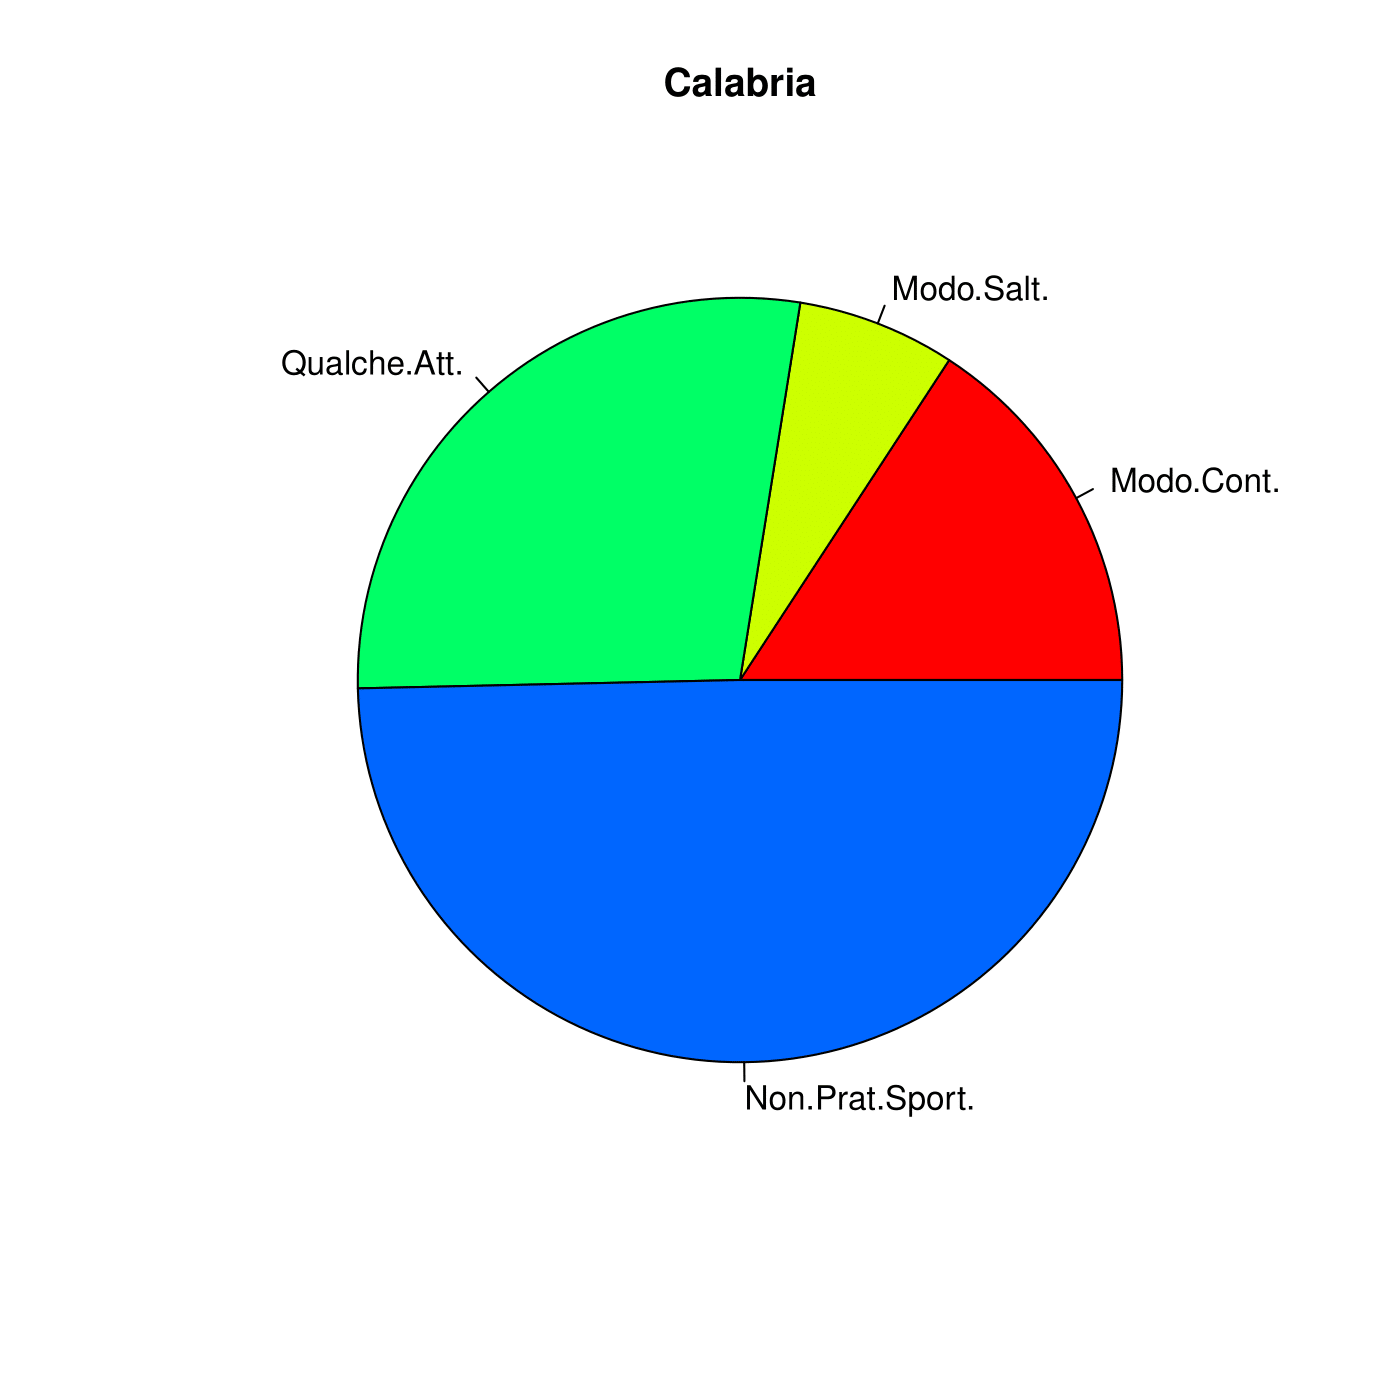
\includegraphics[height=8cm]{ProgettoSAD/capitoli/images/torta_regioni/torta_calabria.png}}
        \qquad
\end{figure}
\begin{figure}[!htbp]
    \centering
        \subfloat{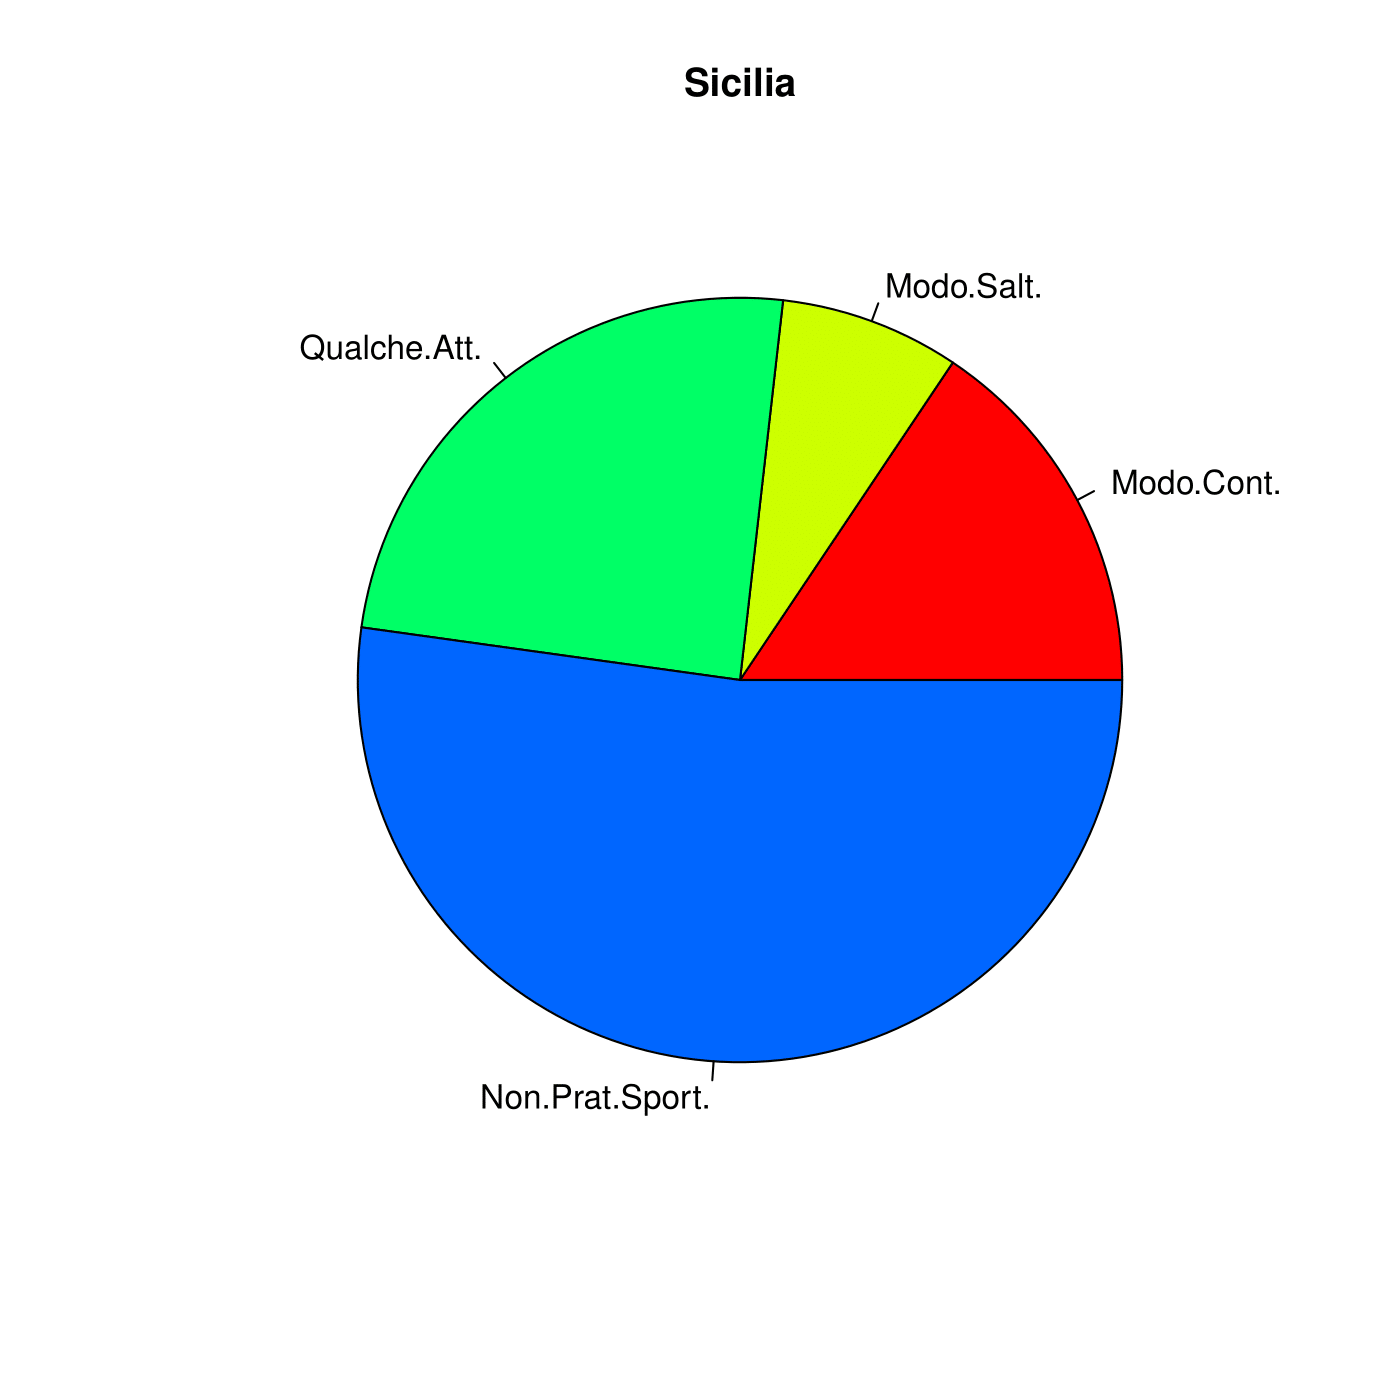
\includegraphics[height=8cm]{ProgettoSAD/capitoli/images/torta_regioni/torta_sicilia.png}}
        \qquad
        \subfloat{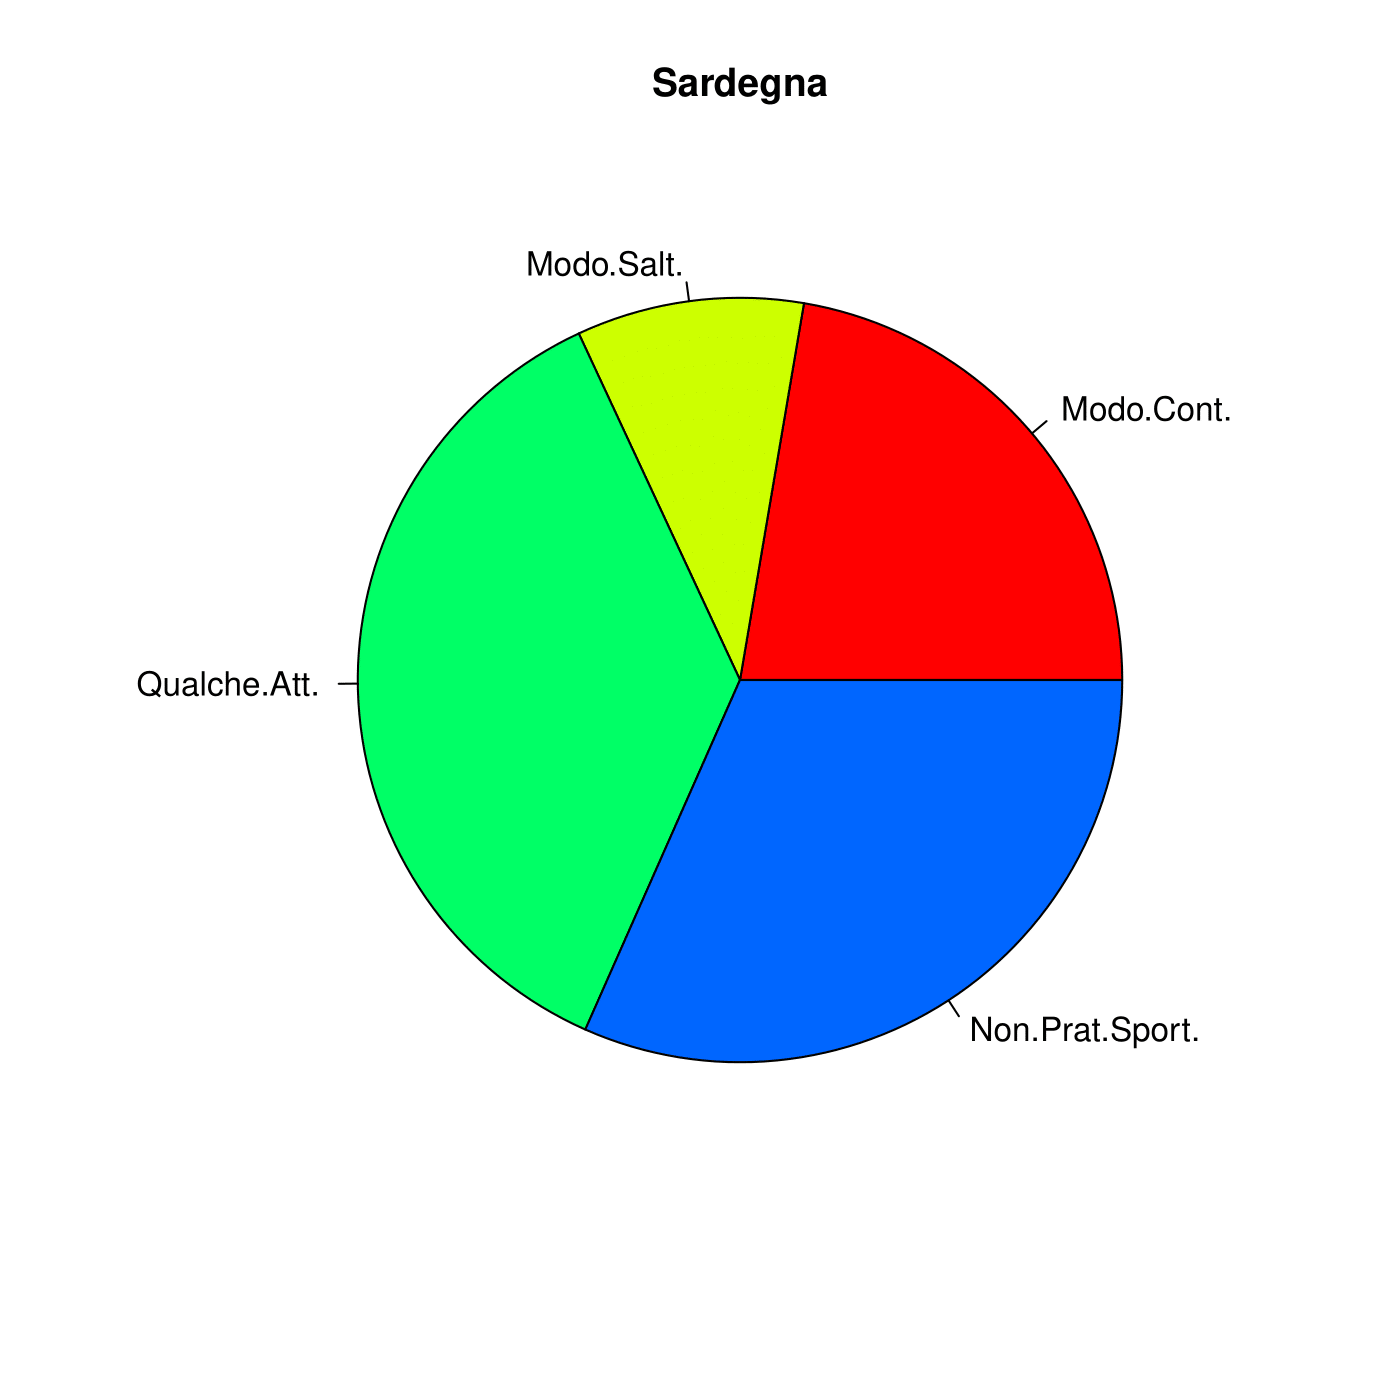
\includegraphics[height=8cm]{ProgettoSAD/capitoli/images/torta_regioni/torta_sardegna.png}}
        \qquad
\end{figure}

Dai grafici a torta disegnati possiamo trarre le stesse conclusioni ottenute 
per i grafici a barre rispetto le caratteristiche.

%################################################

\newpage